%% 
%% Copyright 2007-2024 Elsevier Ltd
%% 
%% This file is part of the 'Elsarticle Bundle'.
%% ---------------------------------------------
%% 
%% It may be distributed under the conditions of the LaTeX Project Public
%% License, either version 1.3 of this license or (at your option) any
%% later version.  The latest version of this license is in
%%    http://www.latex-project.org/lppl.txt
%% and version 1.3 or later is part of all distributions of LaTeX
%% version 1999/12/01 or later.
%% 
%% The list of all files belonging to the 'Elsarticle Bundle' is
%% given in the file `manifest.txt'.
%% 
%% Template article for Elsevier's document class `elsarticle'
%% with numbered style bibliographic references
%% SP 2008/03/01
%% $Id: elsarticle-template-num.tex 249 2024-04-06 10:51:24Z rishi $
%%
\documentclass[preprint,12pt]{elsarticle}

%% Use the option review to obtain double line spacing
%% \documentclass[authoryear,preprint,review,12pt]{elsarticle}

%% Use the options 1p,twocolumn; 3p; 3p,twocolumn; 5p; or 5p,twocolumn
%% for a journal layout:
%% \documentclass[final,1p,times]{elsarticle}
%% \documentclass[final,1p,times,twocolumn]{elsarticle}
%% \documentclass[final,3p,times]{elsarticle}
%% \documentclass[final,3p,times,twocolumn]{elsarticle}
%% \documentclass[final,5p,times]{elsarticle}
%% \documentclass[final,5p,times,twocolumn]{elsarticle}

%% For including figures, graphicx.sty has been loaded in
%% elsarticle.cls. If you prefer to use the old commands
%% please give \usepackage{epsfig}

%% The amssymb package provides various useful mathematical symbols
\usepackage{amssymb}
%% The amsmath package provides various useful equation environments.
\usepackage{amsmath}
%% The amsthm package provides extended theorem environments
%% \usepackage{amsthm}

%% The lineno packages adds line numbers. Start line numbering with
%% \begin{linenumbers}, end it with \end{linenumbers}. Or switch it on
%% for the whole article with \linenumbers.
%% \usepackage{lineno}

\usepackage[ruled,vlined]{algorithm2e}
\usepackage{booktabs}
\usepackage{subcaption}
\usepackage{eurosym}
\usepackage{pdflscape}
\usepackage{tabularx}

\journal{Journal of Energy Storage}

\begin{document}

\begin{frontmatter}

%% Title, authors and addresses

%% use the tnoteref command within \title for footnotes;
%% use the tnotetext command for theassociated footnote;
%% use the fnref command within \author or \affiliation for footnotes;
%% use the fntext command for theassociated footnote;
%% use the corref command within \author for corresponding author footnotes;
%% use the cortext command for theassociated footnote;
%% use the ead command for the email address,
%% and the form \ead[url] for the home page:
%% \title{Title\tnoteref{label1}}
%% \tnotetext[label1]{}
%% \author{Name\corref{cor1}\fnref{label2}}
%% \ead{email address}
%% \ead[url]{home page}
%% \fntext[label2]{}
%% \cortext[cor1]{}
%% \affiliation{organization={},
%%             addressline={},
%%             city={},
%%             postcode={},
%%             state={},
%%             country={}}
%% \fntext[label3]{}

\title{Degradation-Aware Planning of Shared Battery Energy Storage Systems for Coordinated Transmission and Distribution System Operation}

%% use optional labels to link authors explicitly to addresses:
%% \author[label1,label2]{}
%% \affiliation[label1]{organization={},
%%             addressline={},
%%             city={},
%%             postcode={},
%%             state={},
%%             country={}}
%%
%% \affiliation[label2]{organization={},
%%             addressline={},
%%             city={},
%%             postcode={},
%%             state={},
%%             country={}}

\author[inesctec,feup_ses]{Micael Simões}
\author[inesctec,feup_dee,feup_ses]{João Peças Lopes}
\author[inesctec,feup_dee]{Filipe Joel Soares}

\affiliation[inesctec]{organization={INESC TEC, Center for Power and Energy Systems},
            addressline={Campus da Faculdade de Engenharia da Universidade do Porto, Rua Dr. Roberto Frias}, 
            city={Porto},
            postcode={4200-465}, 
            state={Porto},
            country={Portugal}}

\affiliation[feup_dee]{organization={FEUP, Department of Electrical and Computer Engineering},
            addressline={Rua Dr. Roberto Frias}, 
            city={Porto},
            postcode={4200-465}, 
            state={Porto},
            country={Portugal}}

\affiliation[feup_ses]{organization={FEUP, Sustainable Energy Systems},
            addressline={Rua Dr. Roberto Frias}, 
            city={Porto},
            postcode={4200-465}, 
            state={Porto},
            country={Portugal}}
            

% ====================================================================================================================
%                                                       ABSTRACT                                                      
% ====================================================================================================================
\begin{abstract}
    Energy Storage Systems (ESSs) are an important source of flexibility in power systems with high penetration of Renewable Energy Sources (RESs). When installed at transmission--distribution interface nodes, shared ESSs can support both Transmission System Operators (TSOs) and Distribution System Operators (DSOs), but their long-term planning remains challenging because investment decisions depend on coordinated operation under uncertainty and battery degradation over time.
    This paper proposes a degradation-aware planning framework for shared battery ESSs in coordinated TSO--DSO operation. The problem is formulated as a bi-level stochastic optimization model in which the upper level determines siting, sizing, and staged investment decisions under investment-cost uncertainty, while the lower level evaluates these decisions through coordinated system operation. To preserve tractability, the framework combines Benders' decomposition for long-term planning with an Alternating Direction Method of Multipliers (ADMM)-based decentralized coordination mechanism for short-term operation.
    The framework is evaluated on integrated IEEE transmission--distribution test systems over a 15-year planning horizon. Relative to uncoordinated operation, coordinated operation with shared ESSs reduces operating costs by up to 18.25\% and RES curtailment by up to 92.16\% in the later years of the planning horizon, while eliminating voltage violations. The results also show that degradation materially affects ESS valuation and that temporal discretization can influence siting and sizing decisions.
\end{abstract}


%%Graphical abstract
% ====================================================================================================================
%                                                  GRAPHICAL ABSTRACT                                                 
% ====================================================================================================================
\begin{graphicalabstract}
    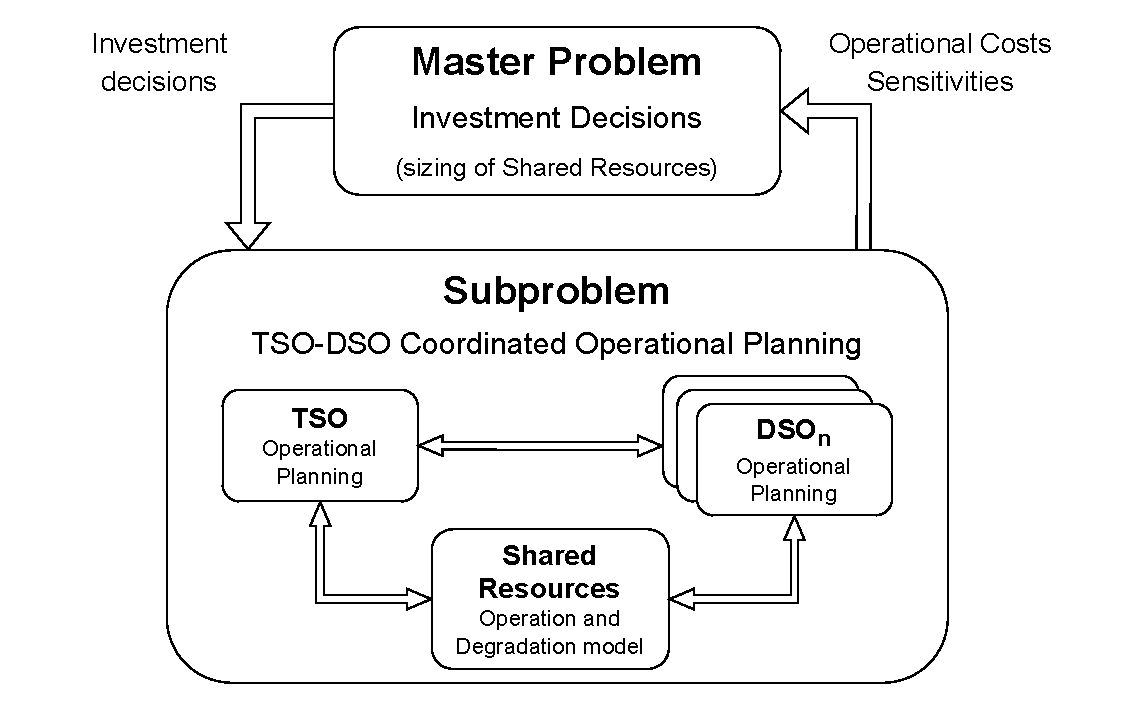
\includegraphics[width=1.00\textwidth]{framework.pdf}
\end{graphicalabstract}


\begin{highlights}
    \item A bi-level stochastic framework is proposed for planning shared ESSs at TN--DN interface nodes
    \item Cycling-induced battery degradation is explicitly linked to coordinated multi-year TSO--DSO operation
    \item Benders' decomposition and ADMM enable scalable planning with decentralized AC-feasible operation
    \item Shared ESSs reduce operating costs, RES curtailment, and voltage violations under coordinated operation
    \item Planning-horizon discretization materially affects degradation trajectories and ESS investment decisions
\end{highlights}


\begin{keyword}
    Shared energy storage systems \sep
    Battery degradation \sep
    Bi-level stochastic optimization \sep
    TSO--DSO coordination \sep
    Benders' decomposition \sep
    ADMM
\end{keyword}

\end{frontmatter}

%% Add \usepackage{lineno} before \begin{document} and uncomment 
%% following line to enable line numbers
%% \linenumbers

% ====================================================================================================================
%                                                     NOMENCLATURE                                                    
% ====================================================================================================================
\section*{Nomenclature}

\subsection*{Sets and Parameters}

\begin{table}[htbp!]
    \centering
    \begin{tabular}{l l}
        \toprule
        \textbf{Symbol} & \textbf{Description} \\
        \midrule    
        \multicolumn{2}{l}{\textbf{Sets}}\\
        $E^S$       & Set of shared ESSs \\
        $Y$         & Set of representative years \\
        $D$         & Set of representative days \\
        $T$         & Set of intra-day time instants \\
        $\Omega_C$  & Set of investment-cost scenarios \\     
        $L^B$       & Set of Benders' iterations\\
        \midrule
        \multicolumn{2}{l}{\textbf{Parameters}}\\
        $\omega_c$ & Probability of investment-cost scenario $c \in \Omega_C$ \\
        $c^{\text{Inv,S}}_{y,c}$ & Unit investment cost of converter power rating in year $y$ and \\
        ~                        & investment scenario $c$\\
        $c^{\text{Inv,E}}_{y,c}$ & Unit investment cost of energy capacity in year $y$ and \\
        ~                        & investment scenario $c$\\        
        $T^\text{Cal}_{e,y}$ & Calendar lifetime of ESS $e$ installed in year $y$ \\
        $E^{\text{Max}}_{e,y}$ & Maximum installable energy capacity of unit $e$ in year $y$ \\
        $\phi^{\text{Min}}_e$ & Minimum admissible energy-to-power ratio of unit $e$ in year $y$ \\
        $\phi^{\text{Max}}_e$ & Maximum admissible energy-to-power ratio of unit $e$ in year $y$ \\
        $c^{\text{Inv}}$ & Total investment budget \\
        $\alpha^{\text{Down}}$ & Lower bound on the Benders underestimator \\
        $SoH_{e,y}^{\text{min}}$ & Minimum admissible SoH of unit $e$ in year $y$ \\
        $D_d$ & Number of calendar days represented by $d \in D$ \\
        $Y_y$ & Number of calendar years represented by $y \in Y$ \\
        $\mathrm{CL}^\text{Nom}_e$ & Nominal cycle life of unit $e \in E^S$\\
        $r$   & Discount rate\\      
        \bottomrule
    \end{tabular}
\end{table}

\subsection*{Variables}

\begin{table}[htbp!]
    \centering
    \begin{tabular}{l l}
        \toprule
        \textbf{Variable} & \textbf{Description} \\
        \midrule
        $S^{\text{Inv}(l)}_{e,y,c}$ & Scenario-dependent investment in converter power rating in \\
        ~                           & ESS $e$ in year $y$ and investment scenario $c$\\
        $E^{\text{Inv}(l)}_{e,y,c}$ & Scenario-dependent investment in energy capacity in ESS $e$ \\
        ~                           & in year $y$ and investment scenario $c$\\
        $S^{\text{Rated}}_{e,y^\text{Inv},y}$   & Rated power of unit $e$ installed in year $y^\text{Inv}$ \\
        ~                                       & and operated in year $y$ \\
        $E^{\text{Rated}}_{e,y^\text{Inv},y}$ & Available energy capacity of unit $e$ installed in year $y^\text{Inv}$\\
        ~                                       & and operated in year $y$ \\
        $S^{\text{Av,Unit}}_{e,y^\text{Inv},y}$ & Available power of unit $e$ installed in year $y^\text{Inv}$ \\
        ~                                       & and operated in year $y$ \\
        $E^{\text{Av,Unit}}_{e,y^\text{Inv},y}$ & Available energy capacity of unit $e$ installed in year $y^\text{Inv}$\\
        ~                                       & and operated in year $y$ \\
        $SoH_{e,y^\text{Inv},y}$ & SoH of unit $e$ installed in year $y^\text{Inv}$ and operated in year $y$ \\
        $\delta_{e,y^\text{Inv},y}$ & Average equivalent daily degradation rate of unit $e$ installed \\
        ~                           & in year $y^\text{Inv}$ and operated in year $y$ \\
        $S^\text{Ch}_{e,y^\text{Inv},y,d,t}$ & Charging apparent power of unit $e$, installed in year $y^\text{Inv}$ and\\
        ~                                    & operated in year $y$, representative day $d$, time instant $t$\\
        $S^\text{Dch}_{e,y^\text{Inv},y,d,t}$ & Discharging apparent power of unit $e$, installed in year $y^\text{Inv}$\\
        ~                                     & and operated in year $y$, representative day $d$, time instant $t$\\
        $P^{\text{Net}}_{e,y,d,t}$ & Net active power request to unit $e$ in year $y$, representative \\
        ~                          & day $d$, and time instant $t$, issued by the SOs participating in\\
        ~                          & the coordination procedure\\
        $Q^{\text{Net}}_{e,y,d,t}$ & Net reactive power request to unit $e$ in year $y$, representative \\
        ~                          & day $d$, and time instant $t$, issued by the SOs participating in\\
        ~                          & the coordination procedure\\
        \bottomrule
    \end{tabular}
\end{table}

\newpage

% ====================================================================================================================
%                                                     INTRODUCTION                                                    
% ====================================================================================================================
\section{Introduction}

Energy Storage Systems (ESSs) are becoming a key enabler of low-carbon power systems by providing temporal flexibility, supporting Renewable Energy Sources (RESs) integration, and improving the secure operation of increasingly decentralized electricity networks. Beyond short-term balancing, ESSs provide value across multiple timescales through congestion management, voltage support, peak shaving, and reserve provision. Consequently, determining where storage should be installed, how large it should be, and how it should be operated over its lifetime has become a central problem in modern power-system planning and operation.

This challenge is particularly relevant in power systems with high penetration of Distributed Energy Resources (DERs), where interactions between transmission and distribution networks are becoming more pronounced. As conventional synchronous generation is progressively displaced by RESs, system controllability and operational security increasingly depend on coordinated flexibility activation across both network levels. In this context, effective coordination between Transmission System Operators (TSOs) and Distribution System Operators (DSOs) is essential for secure, reliable, and economically efficient system operation under growing decentralization and uncertainty~\cite{eu_regulation_2017,eu_regulation_2019}. 
Despite strong regulatory and academic interest, practical TSO--DSO coordination remains limited~\cite{cadre_2019}. Most existing mechanisms focus on short-term operational interactions and overlook the long-term planning implications of flexibility deployment, which can lead to investment decisions that are suboptimal under realistic operating conditions.

In this setting, ESSs installed at Transmission Network (TN)--Distribution Network (DN) interface nodes constitute an attractive shared flexibility resource. When jointly managed by TSOs and DSOs, shared ESSs can support congestion management, voltage regulation, RES integration, and balancing services across both network levels~\cite{simoes_2025}. Their planning, however, introduces several methodological challenges. Battery-based ESSs are subject to degradation, so operational decisions affect not only short-term system performance but also long-term usable capacity and asset lifetime. In addition, realistic evaluation of shared ESS performance in coordinated TN--DN operation requires nonlinear AC network modeling, while institutional independence and data privacy constraints motivate decentralized solution approaches~\cite{capitanescu_2016,usman_2023}. These aspects are rarely addressed simultaneously in existing planning frameworks.

Early studies on ESS siting and sizing primarily considered centralized settings and relied on heuristic methods, simplified network models, or single-level optimization frameworks. Although later works introduced multi-stage and bi-level formulations, several important limitations remain. 
First, many studies do not represent TN and DNs under detailed AC power flow constraints~\cite{massucco_2021,hassan_2018,feng_2025,najibi_2021,nawaz_2021,papalexopoulos_2020,bragin_2022,qiu_2017}. 
Second, a large share of the literature assumes one-time fixed-capacity investments, thereby neglecting the staged and modular nature of battery-based storage expansion~\cite{pandzic_2015,liu_2016,li_2015,bayram_2017,zhang_2013,hedayati_2014,konstantelos_2015}. 
Third, battery degradation is often neglected or represented through simplified heuristics that do not explicitly link operational cycling to long-term usable capacity~\cite{liu_2016,li_2015,bayram_2017,zhang_2013,hedayati_2014,konstantelos_2015,nasrolahpour_2016,xu_2017,motalleb_2016,feng_2025,pandzic_2015,fortenbacher_2016,nick_2018}. 
Finally, decentralized TSO--DSO coordination mechanisms are rarely integrated into long-term storage planning despite the practical relevance of institutional separation and data privacy.

Overall, the literature still lacks an integrated framework that simultaneously addresses four key requirements of long-term shared ESS planning: 
(i) siting and sizing of shared storage at TN--DN interface nodes, 
(ii) explicit representation of cycling-induced battery degradation, 
(iii) AC-feasible coordinated TSO--DSO operation, and 
(iv) decentralized solution mechanisms compatible with institutional separation and data privacy constraints. 
Addressing these aspects jointly is essential to obtain economically meaningful and technically feasible shared ESS investment strategies.

To address this gap, this paper proposes a bi-level optimization framework for planning shared ESSs installed at TN--DN interface nodes. The upper level determines siting, sizing, and staged investment decisions under investment-cost uncertainty. The lower level evaluates these decisions through a coordinated TSO--DSO operational planning model based on the Alternating Direction Method of Multipliers (ADMM) framework introduced in~\cite{simoes_2023}, extended here to explicitly incorporate battery degradation. The resulting formulation combines stochastic planning, nonlinear AC network modeling, and decentralized coordination within a scalable decomposition structure, thereby linking long-term ESS expansion decisions with short-term storage utilization in an AC-feasible and degradation-aware setting.

The main contributions of this paper are as follows:
\begin{itemize}
    \item A bi-level stochastic planning framework for shared ESS deployment at TN--DN interface nodes that links long-term investment decisions with short-term coordinated TSO--DSO operation.
    \item A degradation-aware shared ESS formulation that internalizes cycling-induced capacity loss in long-term planning decisions and preserves intertemporal consistency of available storage capacity.
    \item A decomposition-based solution strategy that combines Benders' decomposition at the planning level with an ADMM-based decentralized coordination mechanism for AC-feasible TSO--DSO operation.
    \item An extensive case study demonstrating the operational and planning value of shared ESSs relative to benchmark configurations without coordination and without shared storage, together with a sensitivity analysis of planning-horizon discretization.
\end{itemize}

%The results show that coordinated planning and operation with shared ESSs yield substantial system-wide benefits, including lower operating costs, improved RES integration, and mitigation of voltage violations observed under uncoordinated operation. They also show that explicitly representing degradation materially affects ESS valuation and long-term investment outcomes, while planning-horizon discretization can influence degradation trajectories and, consequently, ESS siting and sizing decisions.

The remainder of the paper is organized as follows: 
Section~\ref{sec:methodology} presents the proposed bi-level planning framework and solution methodology;
Section~\ref{sec:case_studies} describes the case study;
Section~\ref{sec:results} discusses the numerical results; and 
Section~\ref{sec:conclusions} concludes the paper and outlines future research directions.


% ====================================================================================================================
%                                                      METHODOLOGY                                                    
% ====================================================================================================================
\section{Shared ESS Planning Framework}
\label{sec:methodology}

The proposed framework is formulated as a bi-level optimization problem. The upper level determines long-term investment decisions, while the lower level evaluates them through coordinated TSO--DSO operation under representative operating conditions. The framework supports staged ESS expansion, reflecting the modular nature of battery-based storage technologies, and explicitly represents battery degradation, thereby linking short-term ESS utilization with long-term available capacity.

To preserve physical fidelity while maintaining computational tractability, a two-layer decomposition strategy is adopted. The outer layer represents the investment planning problem and is solved by Benders' decomposition~\cite{conejo_2006}, whereas the inner layer captures coordinated short-term operation through the ADMM-based framework introduced in~\cite{simoes_2023}. This structure enables scalable multi-year planning while retaining detailed AC network modeling and institutional decoupling among System Operators (SOs). 
Battery degradation is represented through a throughput-based model that captures the dominant effect of cycling on usable energy capacity while abstracting from detailed electrochemical aging mechanisms.

\subsection{Bi-Level Planning Architecture}

Figure~\ref{fig:bilevel_tool_framework} illustrates the proposed architecture. The master problem determines the location, size, and timing of shared ESS investments at TN--DN interface nodes over the planning horizon. For each candidate investment plan, the subproblem evaluates coordinated TSO--DSO operation under representative operating conditions while explicitly tracking ESS degradation across representative years.

\begin{figure}[htbp!]
    \centering
    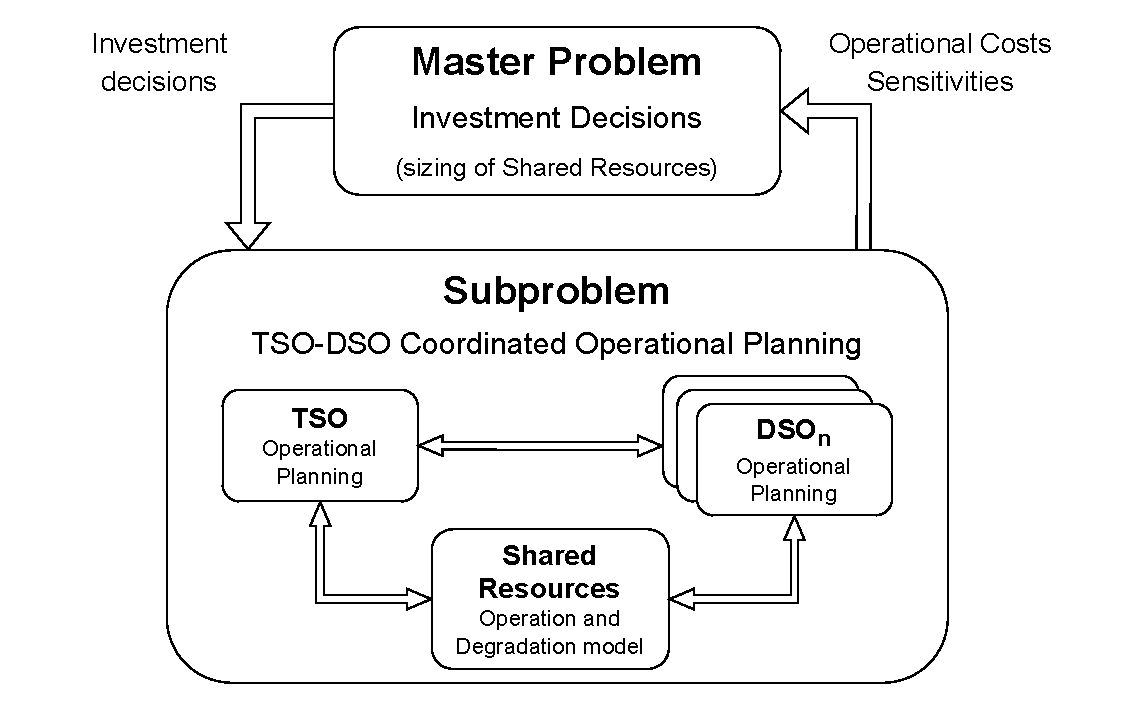
\includegraphics[width=1.00\textwidth]{framework.pdf}
    \caption{Bi-level planning framework.}
    \label{fig:bilevel_tool_framework}
\end{figure}

The two layers are coupled through the ESS investment variables. Benders' decomposition iteratively updates these variables until convergence between strategic planning and operational performance is achieved. To represent long-term storage aging without sacrificing decomposition across SOs, the operational layer includes a dedicated \textit{shared ESS agent} that tracks State-of-Health (SoH) and the resulting evolution of available energy capacity. This preserves decomposition of the TSO and DSO subproblems across representative years while maintaining intertemporal consistency of ESS degradation over the planning horizon.

\subsection{Master Problem}

At the master level, the framework determines strategic investment decisions for shared ESSs at TN--DN interface nodes, including siting, sizing, and staged capacity expansion over the planning horizon. Investment-cost uncertainty is represented through a set of cost trajectories. The master problem evaluates investment decisions under these trajectories and computes the corresponding scenario-weighted expected investment levels used in the lower-level operational evaluation. %Under this modeling choice, the operational subproblem assesses the expected shared ESS deployment induced by the investment-cost uncertainty representation. This approximation preserves tractability while allowing the planning layer to internalize uncertain investment conditions.

\subsubsection{Objective Function}

The master problem minimizes the expected discounted investment cost of shared ESSs, expressed as:

\begin{equation}
    \min \sum_{e \in E^S} \sum_{y \in Y} \sum_{c \in \Omega_C} 
    \Bigg( 
        \frac{\omega_c}{(1 + r)^{y - y_0}} 
        \left( 
            c^{\text{Inv,S}}_{y,c} S^{\text{Inv}(l)}_{e,y,c} + 
            c^{\text{Inv,E}}_{y,c} E^{\text{Inv}(l)}_{e,y,c} 
        \right)
    \Bigg)
    + \alpha^{(l)}
\end{equation}

\noindent
where 
$c^{\text{Inv,S}}_{y,c}$ and $c^{\text{Inv,E}}_{y,c}$ denote the scenario-dependent unit investment costs of converter power rating and energy capacity, respectively; 
$S^{\text{Inv}(l)}_{e,y,c}$ and $E^{\text{Inv}(l)}_{e,y,c}$ are the corresponding investment decisions; and 
$\alpha^{(l)}$ is an auxiliary variable representing the Benders underestimator of the operational cost term.

\subsubsection{Total Rated Power and Energy Capacity}

The \textit{total} rated power and energy capacity of each shared ESS are cumulative functions of the yearly investments made throughout the planning horizon and are limited by the calendar lifetime of each installation ($\forall e \in E^S$, $\forall y \in Y$, $\forall c \in \Omega_C$, $\forall l \in L^B$):

\begin{equation}
    S^{\text{Rated}(l)}_{e,y,c} = \sum_{y^\text{Inv}=\max(y-T^\text{Cal}_{e,y},\,y_0)}^{y} S^{\text{Inv}(l)}_{e,y^\text{Inv},c}
\end{equation}

\begin{equation}
    E^{\text{Rated}(l)}_{e,y,c} = \sum_{y^\text{Inv}=\max(y-T^\text{Cal}_{e,y},\,y_0)}^{y} E^{\text{Inv}(l)}_{e,y^\text{Inv},c}
\end{equation}

\noindent
where 
$S^{\text{Rated}(l)}_{e,y,c}$ and $E^{\text{Rated}(l)}_{e,y,c}$ denote the total rated power and energy capacity available at node $e$ in year $y$, under investment scenario $c$, at iteration $l$; 
$S^{\text{Inv}(l)}_{e,y^\text{Inv},c}$ and $E^{\text{Inv}(l)}_{e,y^\text{Inv},c}$ denote the corresponding incremental investments in rated power and energy capacity made in year $y^\text{Inv}$; and 
$T^\text{Cal}_{e,y}$ is the calendar lifetime of ESS $e$, installed in year $y$.

\subsubsection{Maximum Installable Capacity}

Each shared ESS is subject to an upper bound on installable energy capacity, reflecting physical, spatial, or technical constraints at the corresponding TN--DN interface substation ($\forall e \in E^S$, $\forall y \in Y$, $\forall c \in \Omega_C$, $\forall l \in L^B$):

\begin{equation}
    E_{e,y,c}^{\text{Rated}(l)} \leq E^{\text{Max}}_{e,y}
\end{equation}

\noindent
where $E^{\text{Max}}_{e,y}$ denotes the maximum installable capacity for ESS $e$ in year $y$.

\subsubsection{Energy-to-Power Capacity Ratio}

Battery-based ESSs are characterized by technology- and application-specific energy-to-power ratios, enforced through the following constraint ($\forall e \in E^S$, $\forall y \in Y$, $\forall c \in \Omega_C$, $\forall l \in L^B$):

\begin{equation}
    \phi^{\text{Min}}_e S^{\text{Inv}(l)}_{e,y,c} \leq 
    E^{\text{Inv}(l)}_{e,y,c} \leq 
    \phi^{\text{Max}}_e S^{\text{Inv}(l)}_{e,y,c}
\end{equation}

\noindent
where 
$\phi^{\text{Min}}_e$ and $\phi^{\text{Max}}_e$ denote the minimum and maximum admissible energy-to-power ratios for shared ESS $e$. 
These bounds constrain storage duration according to the selected technology and use case. Typical values for utility-scale lithium-ion batteries range from 2~h to 10~h~\cite{nrel_ess_costs}.

\subsubsection{Available Budget}

The total discounted investment cost incurred over the planning horizon is constrained by the available budget ($\forall l \in L^B$):

\begin{equation}
    \sum_{e \in E^S} \sum_{y \in Y} \sum_{c \in \Omega_C} 
    \frac{\omega_c}{(1 + r)^{y - y_0}}
    \left(
        c^{\text{Inv,S}}_{y,c} S^{\text{Inv}(l)}_{e,y,c}
        + 
        c^{\text{Inv,E}}_{y,c} E^{\text{Inv}(l)}_{e,y,c}
    \right)
    \leq c^{\text{Inv}}
\end{equation}

\noindent
where $c^{\text{Inv}}$ denotes the total investment budget allocated to shared ESSs.

\subsubsection{Expected Rated Power and Energy Capacity}

The \textit{expected} rated power and energy capacities are defined as probability-weighted averages over all investment-cost scenarios $c \in \Omega_C$ ($\forall e \in E^S$, $\forall y \in Y$, $\forall l \in L^B$):

\begin{equation}
    S^{\text{Rated}(l)}_{e,y} = \sum_{c \in \Omega_C} \omega_c \, S^{\text{Rated}(l)}_{e,y,c}
\end{equation}

\begin{equation}
    E^{\text{Rated}(l)}_{e,y} = \sum_{c \in \Omega_C} \omega_c \, E^{\text{Rated}(l)}_{e,y,c}
\end{equation}

Analogously, the expected investment decisions for rated power and energy capacity are given by ($\forall e \in E^S$, $\forall y \in Y$, $\forall l \in L^B$):

\begin{equation}
    S^{\text{Inv}(l)}_{e,y} = \sum_{c \in \Omega_C} \omega_c \, S^{\text{Inv}(l)}_{e,y,c}
\end{equation}

\begin{equation}
    E^{\text{Inv}(l)}_{e,y} = \sum_{c \in \Omega_C} \omega_c \, E^{\text{Inv}(l)}_{e,y,c}
\end{equation}

These expected investment variables form the coupling variables between the master and operational problems. At each iteration $l \in L^B$, the master problem computes a scenario-aggregated investment plan, which is then passed to the subproblem for coordinated multi-year TSO--DSO operational evaluation.

%In the present formulation, investment-cost uncertainty is represented through scenario-dependent cost coefficients and the corresponding scenario-weighted investment quantities. The operational subproblem is then evaluated using the expected investment plan, which acts as a scenario-aggregated representation of the installed shared ESS capacity. This modeling choice yields a risk-neutral planning approximation that preserves tractability of the bi-level decomposition. Accordingly, the framework should be interpreted as determining an expected long-term shared ESS expansion plan under uncertain investment trajectories, rather than as a fully multi-stage stochastic program with explicit non-anticipativity constraints.

\subsubsection{Benders' Cuts}

The Benders' decomposition procedure iteratively refines the master problem by adding cuts derived from the operational evaluation of candidate investment plans. When the operational subproblem is feasible, an optimality cut is generated from the corresponding sensitivities with respect to the coupling variables ($\forall k = 1, \ldots, l-1$):

\begin{equation}
    \alpha^{(l)} \ge y^{(k)} 
    +
    \sum_{e \in E^S}\sum_{y \in Y}
    \mu^{S(k)}_{e,y}\left(S^{\text{Inv}(l)}_{e,y}-S^{\text{Inv}(k)}_{e,y}\right)
    +
    \sum_{e \in E^S}\sum_{y \in Y}
    \mu^{E(k)}_{e,y}\left(E^{\text{Inv}(l)}_{e,y}-E^{\text{Inv}(k)}_{e,y}\right)
\end{equation}

\noindent
where 
$y^{(k)}$ denotes the subproblem objective value at iteration $k$, and 
$\mu^{S(k)}_{e,y}$ and $\mu^{E(k)}_{e,y}$ are the corresponding sensitivity coefficients associated with the power and energy investment variables.

To preserve subproblem feasibility, the shared ESS subproblem (Subsection~\ref{subsec:subproblem}) includes penalized slack variables. Their activation indicates that the corresponding investment plan is not operationally feasible without relaxing the operational constraints. The associated sensitivity information is then used to discourage similar investment solutions in subsequent iterations ($\forall k = 1, \ldots, l-1$):

\begin{equation}
    0 \geq -y^{(k)} 
    + 
    \sum_{e \in E^S}\sum_{y \in Y}
    \mu^{S(k)}_{e,y} \left( S^{\text{Inv}(l)}_{e,y} - S^{\text{Inv}(k)}_{e,y} \right) 
    + 
    \sum_{e \in E^S}\sum_{y \in Y}
    \mu^{E(k)}_{e,y} \left( E^{\text{Inv}(l)}_{e,y} - E^{\text{Inv}(k)}_{e,y} \right)
\end{equation}

Finally, to prevent numerical instability during the initial iterations, the underestimator is bounded from below as:

\begin{equation}
    \alpha^{(l)} \geq \alpha^{\text{Down}}
\end{equation}

\noindent
where $\alpha^{\text{Down}}$ is a predefined lower bound ensuring numerical stability.

\subsection{Subproblem}
\label{subsec:subproblem}

The operational subproblem is decomposed into one TSO subproblem, a set of DSO subproblems, and a dedicated shared ESS subproblem. For scalability, the formulation is further decomposed across representative years and representative days. In this formulation, inter-year coupling arises exclusively from ESS degradation and is enforced through the shared ESS subproblem. This structure preserves tractability, scalability, data privacy, and regulatory compliance, since each SO relies only on local proprietary information.

\subsubsection{Shared ESS Operation Subproblem}

To capture the intertemporal effects of battery degradation, the ADMM-based coordination framework introduced in~\cite{simoes_2023} is extended with an additional agent representing the shared ESS subproblem. This agent links short-term operating decisions with long-term degradation dynamics by tracking the evolution of State-of-Health (SoH) and available energy capacity across representative years. Algorithm~\ref{alg:operational_planning_degradation}, given in~\ref{app:admm_updated_algorithm}, presents the updated pseudo-code of the coordination procedure, while~\ref{app:admm_updated_implementation} details the corresponding mathematical formulation.

\subsubsection{Shared ESS Mathematical Formulation}

Investment decisions on rated power and energy capacity determined by the master problem are treated as fixed parameters in the subproblem. These decisions are enforced through the following constraints ($\forall e \in E^S$, $\forall y \in Y$):

\begin{equation}
    S^{\text{Inv}}_{e,y} = \hat{S}^{\text{Inv}}_{e,y} + S^{\text{Up}}_{e,y} - S^{\text{Down}}_{e,y}
\end{equation}

\begin{equation}
    E^{\text{Inv}}_{e,y} = \hat{E}^{\text{Inv}}_{e,y} + E^{\text{Up}}_{e,y} - E^{\text{Down}}_{e,y}
\end{equation}

\noindent
where 
$\hat{S}^{\text{Inv}}_{e,y}$ and $\hat{E}^{\text{Inv}}_{e,y}$ denote the expected investments in power rating and energy capacity, respectively, for ESS $e$ in year $y$. 
The variables $S^{\text{Up}}_{e,y}$, $S^{\text{Down}}_{e,y}$, $E^{\text{Up}}_{e,y}$, and $E^{\text{Down}}_{e,y}$ are slack variables introduced to preserve subproblem feasibility under all operating conditions. These slack variables are penalized in the subproblem objective function to discourage deviations from the investment targets determined at the master level.

The rated power and energy capacity of each shared ESS over the planning horizon are determined by investments made in successive representative years. To explicitly capture this evolution, auxiliary variables are introduced to represent the contribution of each investment throughout its operational lifetime ($\forall e \in E^S$, $\forall y^\text{Inv} \in Y$, and $y \in [y^\text{Inv};~y^\text{Inv}+T^\text{Cal}_{e,y^\text{Inv}}]$):

\begin{equation}
    S^{\text{Rated,Unit}}_{e,y^\text{Inv},y} := S^{\text{Inv}}_{e,y^\text{Inv}}
\end{equation}

\begin{equation}
    E^{\text{Rated,Unit}}_{e,y^\text{Inv},y} := E^{\text{Inv}}_{e,y^\text{Inv}}
\end{equation}

\noindent
where 
$S^{\text{Rated,Unit}}_{e,y^\text{Inv},y}$ and $E^{\text{Rated,Unit}}_{e,y^\text{Inv},y}$ denote the rated power and energy capacity contributed in representative year $y$ by the ESS unit installed at node $e$ in investment year $y^\text{Inv}$.

The total rated power and energy capacity in each year are obtained by aggregating all units within their calendar lifetime ($\forall e \in E^S$, $\forall y \in Y$):

\begin{equation}
    S^{\text{Rated}}_{e,y} = \sum_{y^\text{Inv}=\max(y-T^\text{Cal}_{e,y},\,y_0)}^{y} S^{\text{Rated,Unit}}_{e,y^\text{Inv},y}
\end{equation}

\begin{equation}
    E^{\text{Rated}}_{e,y} = \sum_{y^\text{Inv}=\max(y-T^\text{Cal}_{e,y},\,y_0)}^{y} E^{\text{Rated,Unit}}_{e,y^\text{Inv},y}
\end{equation}

The available rated power and energy capacity of each shared ESS unit are determined by its installed capacity and degradation state over time ($\forall e \in E^S$, $\forall y^\text{Inv} \in Y$, $\forall y \in [y^\text{Inv};~y^\text{Inv}+T^\text{Cal}_{e,y^\text{Inv}}]$):

\begin{equation}
    S^{\text{Av,Unit}}_{e,y^\text{Inv},y} = S^{\text{Rated,Unit}}_{e,y^\text{Inv},y}
\end{equation}

\begin{equation}
    E^{\text{Av,Unit}}_{e,y^\text{Inv},y} = E^{\text{Rated,Unit}}_{e,y^\text{Inv},y} \, SoH_{e,y^\text{Inv},y}
\end{equation}

\noindent
where 
$S^{\text{Av,Unit}}_{e,y^\text{Inv},y}$ and $E^{\text{Av,Unit}}_{e,y^\text{Inv},y}$ denote the available rated power and energy capacity, respectively, of unit $e$, installed in year $y^\text{Inv}$ and operated in subsequent year $y$; and 
$SoH_{e,y^\text{Inv},y} \in [0,1]$ denotes the corresponding SoH. 
While the available rated power is assumed constant over the unit lifetime, the available energy capacity decreases proportionally to the SoH.

Cycling-induced degradation is modeled through a representative daily fractional capacity-loss term compounded over the calendar duration represented by each planning year. For each unit $e \in E^S$, installed in year $y^\text{Inv} \in Y$ and operating in year $y \in [y^\text{Inv};~y^\text{Inv}+T^\text{Cal}_{e,y^\text{Inv}}]$, the average daily degradation is defined as:

\begin{equation}
    \delta_{e,y^\text{Inv},y} = 
    \frac{E^{\text{Ch,Dch}}_{e,y^\text{Inv},y}}
    {2 \, \mathrm{CL}^\text{Nom}_e \, E^{\text{Rated,Unit}}_{e,y^\text{Inv},y}}
\end{equation}

\noindent
where $E^{\text{Ch,Dch}}_{e,y^\text{Inv},y}$ denotes the average daily equivalent throughput of unit $e$ in representative year $y$, and $\mathrm{CL}^\text{Nom}_e$ is its nominal cycle life. The degradation model assumes that cycling-induced capacity loss is proportional to equivalent charge--discharge throughput and inversely proportional to nominal cycle life. Here, throughput is measured on an apparent-energy basis to capture combined active- and reactive-power utilization of the ESS.

The equivalent throughput is obtained from the weighted contribution of all representative days and intra-day time intervals in each representative year. For a unit $e \in E^S$ installed in year $y^\text{Inv} \in Y$ and operated in year $y \in [y^\text{Inv};~y^\text{Inv}+T^\text{Cal}_{e,y^\text{Inv}}]$, this quantity is given by:

\begin{equation}
    E^{\text{Ch,Dch}}_{e,y^\text{Inv},y} = 
    \sum_{d \in D} \sum_{t \in T} 
    \frac{D_d}{365} \, \Delta t \,
    \left(
        S^\text{Ch}_{e,y^\text{Inv},y,d,t}
        + 
        S^\text{Dch}_{e,y^\text{Inv},y,d,t}
    \right)
\end{equation}

\noindent
where 
$D_d$ is the number of calendar days represented by representative day $d$, 
$\Delta t$ is the duration of time instant $t$, and 
$S^\text{Ch}_{e,y^\text{Inv},y,d,t}$ and $S^\text{Dch}_{e,y^\text{Inv},y,d,t}$ denote the charging and discharging apparent powers, respectively. 
The weighting factor $D_d/365$ converts the representative-day schedule into an average daily throughput for representative year $y$. Apparent power is used as an aggregate operational-stress proxy, so that simultaneous provision of active and reactive power contributes to the utilization measure driving degradation. 
%This approximation is particularly relevant in the present TSO--DSO coordination setting, where shared ESSs provide both active- and reactive-power support.

The SoH of each shared ESS unit is a function of its previous SoH and the degradation incurred during the representative year ($\forall e \in E^S$, $\forall y^\text{Inv} \in Y$, $\forall y \in [y^\text{Inv};~y^\text{Inv}+T^\text{Cal}_{e,y^\text{Inv}}]$):

\begin{equation}
    SoH_{e,y^\text{Inv},y} = SoH_{e,y^\text{Inv},y - 1} \left( 1 - \delta_{e,y^\text{Inv},y} \right)^{365 \times Y_y}
    \label{eq:soh_definition}
\end{equation}

\noindent
where $Y_y$ is the number of years represented by representative year $y$. 
For newly installed units, the initial SoH is set to $SoH_{e,y^\text{Inv},y^\text{Inv}-1}=1$.

A minimum SoH constraint is imposed to ensure that each shared ESS retains an acceptable level of usable capacity throughout the planning horizon. For every unit $e \in E^S$, installed in investment year $y^\text{Inv} \in Y$ and operating in subsequent year $y \in [y^\text{Inv};~y^\text{Inv} + T^\text{Cal}_{e,y^\text{Inv}}]$, the constraint is defined as:

\begin{equation}
    SoH_{e,y^\text{Inv},y} \geq SoH_{e,y^\text{Inv}}^{\text{min}}
\end{equation}

\noindent
where $SoH_{e,y^\text{Inv}}^{\text{min}}$ denotes the minimum admissible SoH for unit $e$ installed in year $y^\text{Inv}$.

Charging--discharging complementarity constraints ensure that each ESS cannot simultaneously charge and discharge at any given time instant ($\forall e \in E^S$, $\forall y^\text{Inv} \in Y$, $\forall y \in [y^\text{Inv};~y^\text{Inv}+T^\text{Cal}_{e,y^\text{Inv}}]$, $\forall d \in D$, $\forall t \in T$):

\begin{equation}
    S^\text{Ch}_{e,y^\text{Inv},y,d,t} \, S^\text{Dch}_{e,y^\text{Inv},y,d,t} = 0
    \label{eq:ess_complementarity}
\end{equation}

Although nonconvex, this complementarity formulation avoids binary variables and preserves a continuous nonlinear representation of the shared ESS operation problem. In practice, however, the resulting nonconvexity may affect numerical robustness, so the relaxed formulation in~\eqref{eq:ess_complementarity_relaxed} is used when needed to improve convergence:

\begin{equation}
    S^\text{Ch}_{e,y^\text{Inv},y,d,t} \, S^\text{Dch}_{e,y^\text{Inv},y,d,t} \leq S^\text{S,Comp}_{e,y^\text{Inv},y,d,t}
    \label{eq:ess_complementarity_relaxed}
\end{equation}

\noindent
where $S^\text{S,Comp}_{e,y^\text{Inv},y,d,t}$ is an auxiliary slack variable penalized in the objective function, as described hereafter.

The net apparent power exchanged by each ESS is obtained by aggregating contributions from all active units ($\forall e \in E^S$, $\forall y \in Y$, $\forall d \in D$, $\forall t \in T$): 

\begin{equation}
    S^\text{Net}_{e,y,d,t} =
    \sum_{y^\text{Inv}=\max(y-T^\text{Cal}_{e,y},\,y_0)}^{y}
    \left(
        S^\text{Ch}_{e,y^\text{Inv},y,d,t}
        -
        S^\text{Dch}_{e,y^\text{Inv},y,d,t}
    \right)
\end{equation}

\noindent
which is related to the active and reactive power requests of the SOs by ($\forall e \in E^S$, $\forall y \in Y$, $\forall d \in D$, $\forall t \in T$):

\begin{equation}
    \left(S^{\text{Net}}_{e,y,d,t}\right)^2 =
    \left(P^{\text{Net}}_{e,y,d,t}\right)^2 +
    \left(Q^{\text{Net}}_{e,y,d,t}\right)^2
\end{equation}

\noindent
where $P^{\text{Net}}_{e,y,d,t}$ and $Q^{\text{Net}}_{e,y,d,t}$ denote the net active and reactive power requests, respectively, issued by the SOs participating in the coordination procedure. Note that power-converter-related constraints, such as power-factor limits, are already enforced within the SO models.

The objective of the shared ESS subproblem is auxiliary within the ADMM coordination procedure. It penalizes deviations from the investment targets received from the master problem, as well as violations of the relaxed complementarity condition, thereby steering the subproblem toward a physically consistent and investment-compliant operating point:

\begin{align}
    \min \quad
    & \sum_{e \in E^S} \sum_{y \in Y}
    \left(
        S^{\text{Up}}_{e,y} +
        S^{\text{Down}}_{e,y} +
        E^{\text{Up}}_{e,y} +
        E^{\text{Down}}_{e,y}
    \right) \\
    & + \sum_{e \in E^S} \sum_{y^\text{Inv} \in Y} \sum_{y \in Y} \sum_{d \in D} \sum_{t \in T}
    S^\text{S,Comp}_{e,y^\text{Inv},y,d,t}
\end{align}

Accordingly, the objective should be interpreted as a coordination-penalty function that promotes feasibility and consistency with the master-level investment decisions.


% ====================================================================================================================
%                                                      CASE STUDY                                                     
% ====================================================================================================================
\section{Case Study}
\label{sec:case_studies}

The proposed framework is evaluated on an integrated transmission--distribution test system with high RES penetration and coordinated TSO--DSO operation. The test system comprises the IEEE 9-bus transmission network coupled with three Active Distribution Networks (ADNs), each derived from the IEEE 33-bus distribution test system~\cite{zimmerman_2011,ieee_case33}. A representative single-line diagram of the integrated system is shown in Figure~\ref{fig:tso_dso_coordination_cs1_network_diagram}. 
Shared ESSs can be installed at the TN--DN interface nodes corresponding to the connection points of the three ADNs. The 15-year planning horizon is represented by five years (2025, 2028, 2031, 2034, and 2037), spaced at three-year intervals. For each year, four seasonal representative days are used to capture variability in demand and RES generation.

\begin{figure}[htbp]
    \centering
    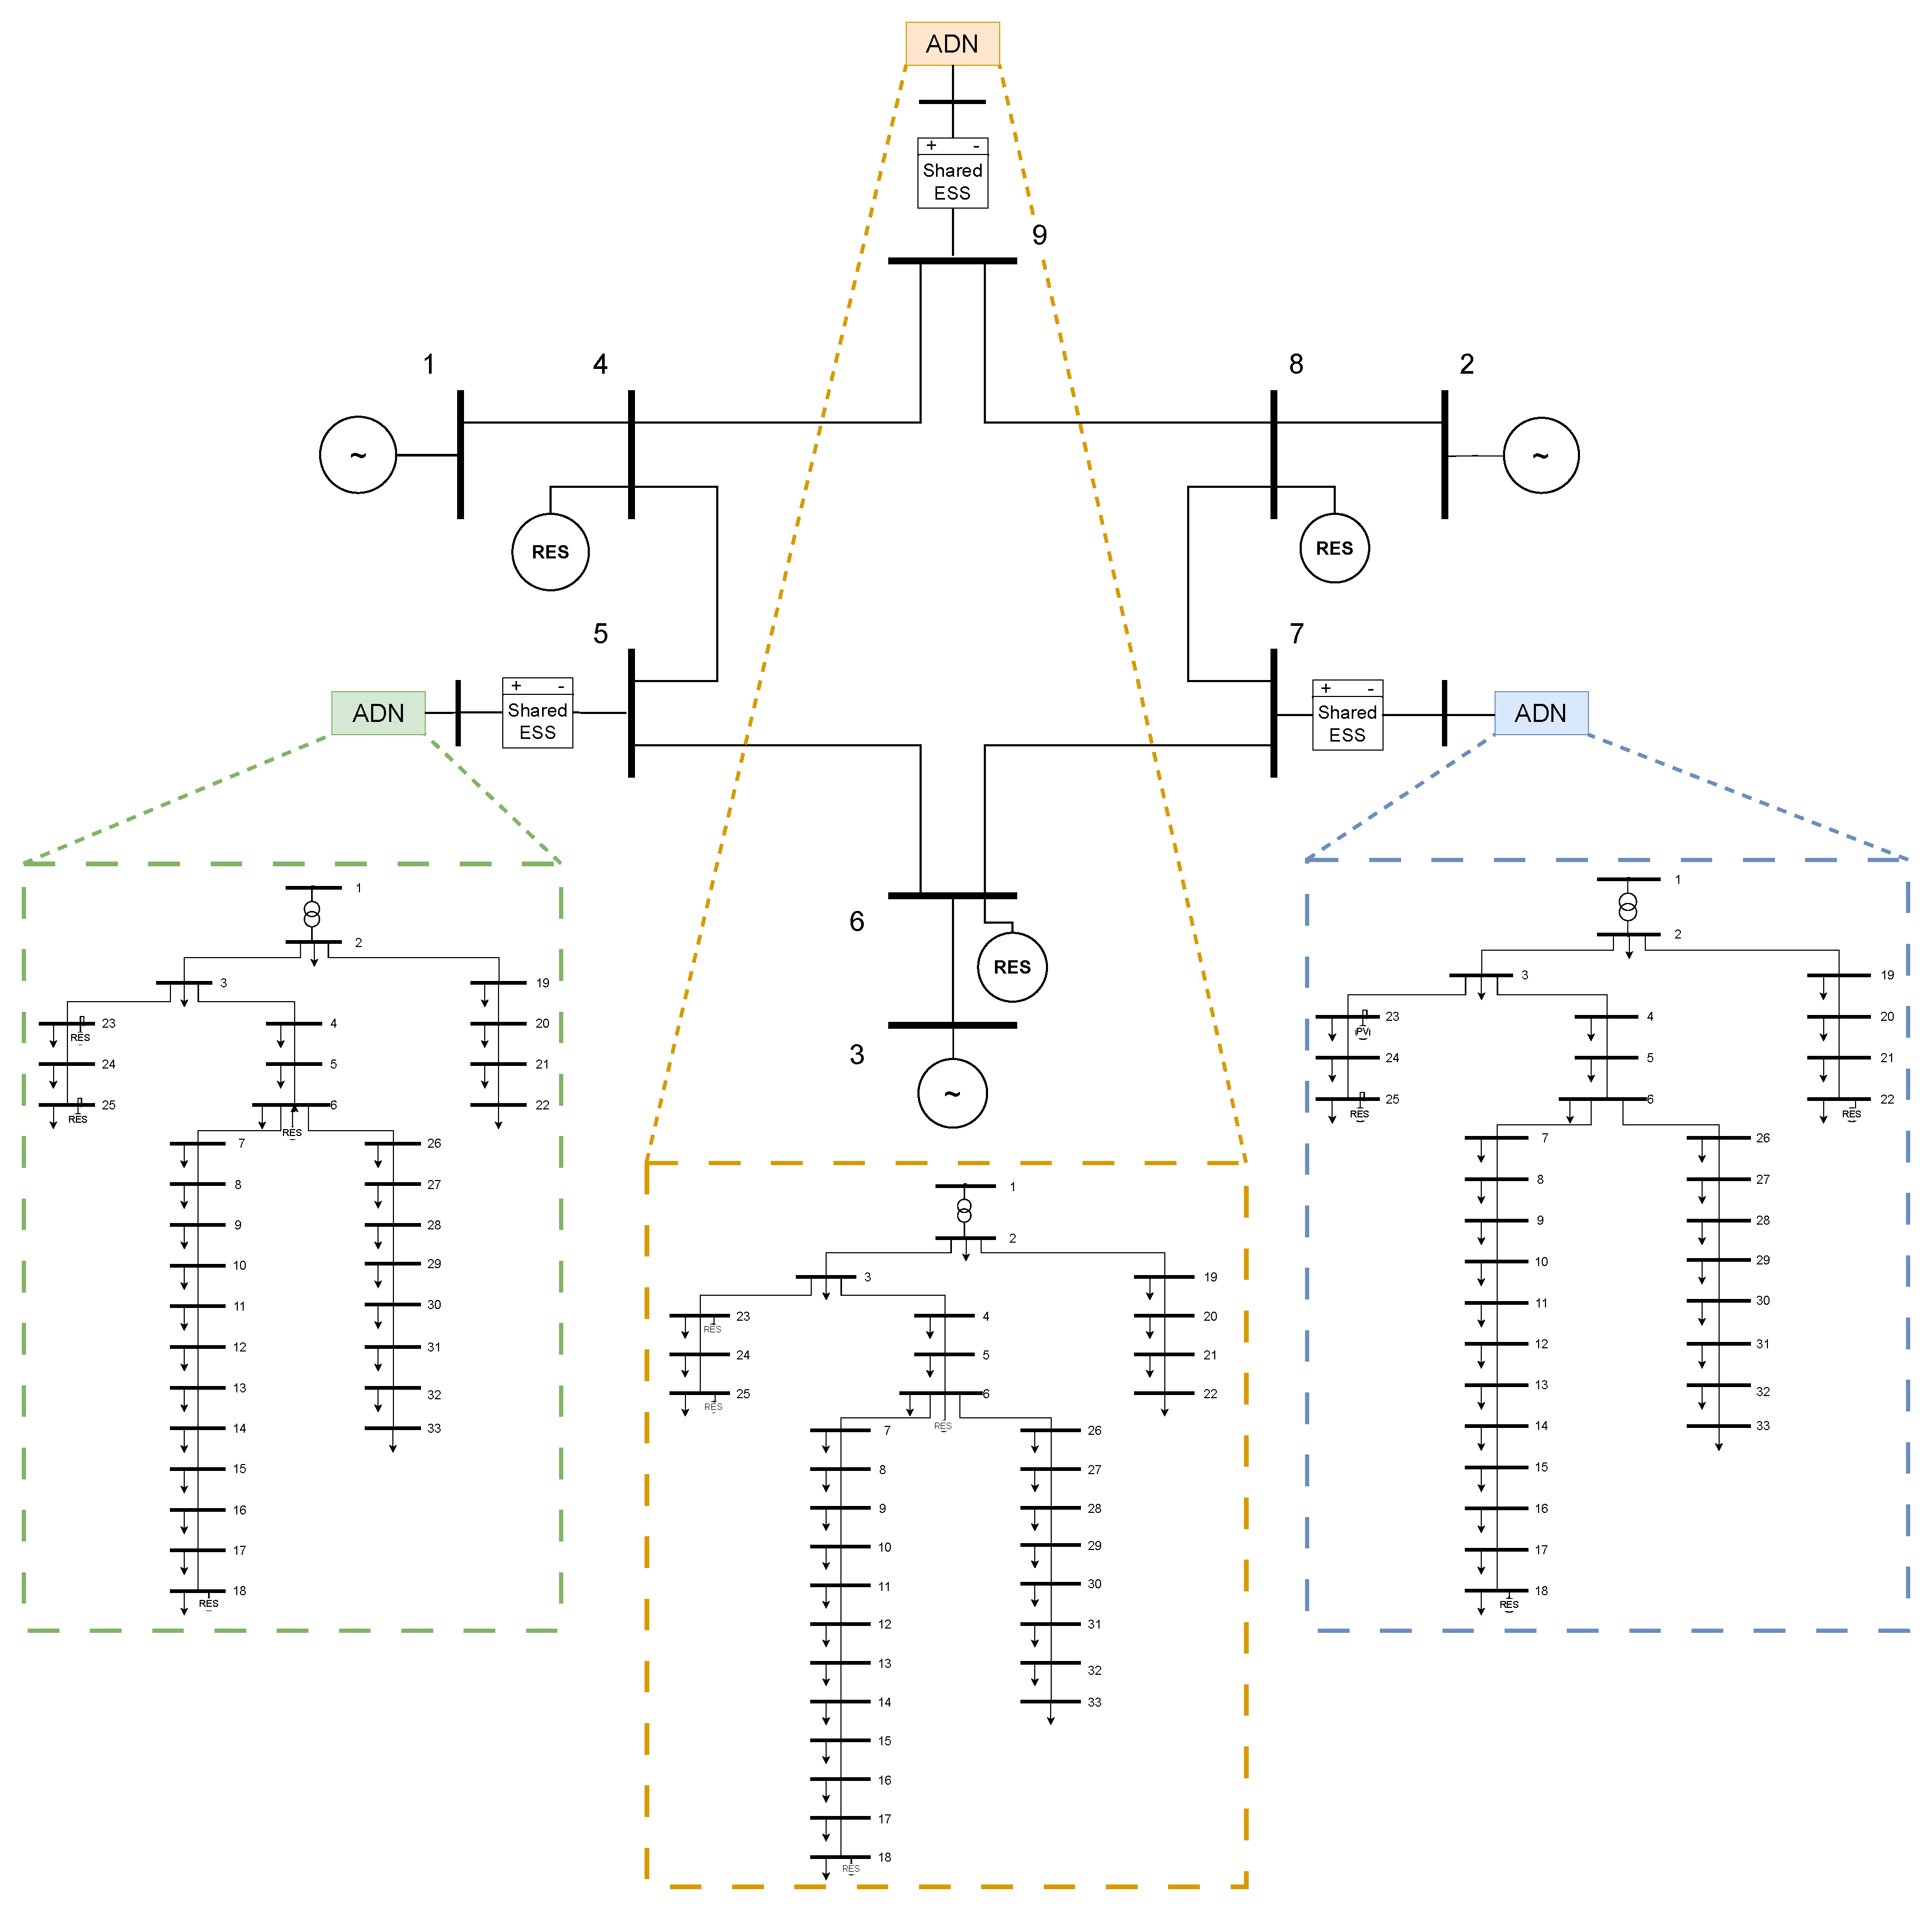
\includegraphics[width=1.00\textwidth]{network_diagram.pdf}
    \caption{Single-line diagram of the adopted test system, including the ADNs participating in the coordination procedure.}
    \label{fig:tso_dso_coordination_cs1_network_diagram}
\end{figure}

Three ESS investment-cost scenarios are considered at the planning level. At the operational level, five load/RES scenarios are combined with five market-price scenarios, resulting in 25 operating scenarios per representative day. The total investment budget for shared ESS deployment is set to 1~M\euro, and the maximum installable energy capacity at each interface node is limited to 5.00~MWh. All shared ESSs are assumed to have a calendar lifetime of 15 years, and a discount rate of 2.00\% is used to compute the Net Present Value (NPV) of all cash flows.

To isolate the value of coordinated operation and the incremental contribution of shared ESS deployment, the proposed framework is benchmarked against two reference cases:
\begin{itemize}
    \item uncoordinated operation, used as a baseline to quantify the overall benefits of TSO--DSO coordination;
    \item coordinated operation without shared ESSs, used to isolate the additional value provided by shared ESS deployment.
\end{itemize}

\subsection{Investment Costs}

To represent uncertainty in future storage costs, three investment trajectories -- low, medium, and high -- are considered, reflecting plausible cost ranges associated with technological progress and market development~\cite{nrel_ess_costs,iea_ess_2024}. The corresponding investment costs are reported in Table~\ref{tab:investment_cost}.

\begin{table}[htbp!]
    \centering
    \caption{Investment costs of shared ESSs~\cite{nrel_ess_costs}.}
    \begin{tabular}{lcc ccccc}
        \toprule
        Parameter & Scn. & Prob., [\%] & 2025 & 2028 & 2031 & 2034 & 2037 \\ 
        \midrule
        $c^\text{Inv,S}_{y,c}$,     & 1 & 35.00\% & 214.17 & 186.90 & 165.76 & 156.88 & 148.01\\ 
        $\left[\text{k\euro/MVA}\right]$ & 2 & 55.00\% & 267.53 & 241.56 & 220.79 & 210.42 & 200.04\\
        ~                           & 3 & 10.00\% & 342.17 & 303.72 & 276.19 & 270.48 & 264.77\\
        \midrule
        $c^\text{Inv,E}_{y,c}$, & 1 & 35.00\% & 169.71 & 148.10 & 131.35 & 124.31 & 117.28\\ 
        $\left[\text{k\euro/MWh}\right]$ & 2 & 55.00\% & 211.99 & 191.41 & 174.95 & 166.73 & 158.51\\ 
        ~                           & 3 & 10.00\% & 271.13 & 240.67 & 218.85 & 214.33 & 209.80\\ 
        \bottomrule
    \end{tabular}
    \label{tab:investment_cost}
\end{table}

%By explicitly modeling multiple investment cost trajectories and their associated probabilities, the proposed planning framework accounts for investment cost uncertainty directly within the optimization process. This enables the model not only to identify the optimal \emph{siting} and \emph{sizing} of shared ESSs, but also to make informed decisions regarding the \emph{timing} of capacity deployment. 

\subsection{Market Data}

Baseline wholesale energy prices were obtained from the Portuguese TSO platform~\cite{ren_market_platform}, whereas flexibility market prices were sourced from the ATTEST project repository~\cite{attest_project_repo}. Seasonal profiles are provided in~\ref{app:market_data}. Wholesale energy prices are assumed to increase at an average annual rate of 2.50\%, whereas flexibility market prices increase at 2.00\% per year.

\subsection{Transmission Network}

The transmission network is based on the IEEE 9-bus test system~\cite{zimmerman_2011}. To reflect increasing RES penetration over the planning horizon, installed wind and solar PV capacities vary across the representative years, as summarized in Table~\ref{tab:cs3_tn_res_generators}. This progressive growth in variable renewable generation creates evolving flexibility needs and provides a suitable setting for evaluating the timing and value of shared ESS deployment. The RES generation profiles adopted for the spring, summer, autumn, and winter representative days of the initial planning year (2025) are provided in~\ref{app:tn_description}.

\begin{table}[htbp!]
    \centering
    \caption{TN installed RES capacity in each representative year.}
    \begin{tabular}{ccc ccccc}
        \toprule
        Generator   & Node  & Generator & \multicolumn{5}{c}{Installed capacity, [MW]}\\  \cmidrule{4-8}
        ID          & ID    & Type      & 2025  & 2028  & 2031  & 2034   & 2037 \\ 
        \midrule
        4 & 4 &  Wind     & 20.00 & 20.00 & 30.00 & 30.00 & 50.00\\
        5 & 6 &  Wind     & 40.00 & 40.00 & 60.00 & 60.00 & 60.00\\
        6 & 8 &  Wind     & 25.00 & 25.00 & 40.00 & 40.00 & 40.00\\
        7 & 4 &  Solar PV & 12.00 & 12.00 & 20.00 & 20.00 & 20.00\\
        8 & 6 &  Solar PV & 20.00 & 20.00 & 30.00 & 30.00 & 50.00\\
        9 & 8 &  Solar PV & 15.00 & 15.00 & 25.00 & 25.00 & 25.00\\
        \bottomrule
    \end{tabular}
    \label{tab:cs3_tn_res_generators}
\end{table}

\subsection{Active Distribution Networks}
\label{subsec:case_study_adns}

The three ADNs share the IEEE 33-bus topology but differ in RES penetration levels and growth trajectories, thereby creating heterogeneous flexibility conditions across the TN--DN interfaces. This heterogeneity allows assessment of how the value of shared ESS deployment depends on local network characteristics. Tables~\ref{tab:cs3_adn_node_5_res_generators}--\ref{tab:cs3_adn_node_9_res_generators} summarize the installed RES capacities for the ADNs connected to TN nodes 5, 7, and 9, respectively. Seasonal RES and load profiles for the base year (2025) are provided in~\ref{app:dns_description}.

\begin{table}[htbp!]
    \centering
    \caption{ADN at TN node~5: installed RES capacity in each representative year.}
    \begin{tabular}{ccc ccccc}
        \toprule
        Generator   & Node  & Generator & \multicolumn{5}{c}{Installed capacity, [MW]}\\  \cmidrule{4-8}
        ID          & ID    & Type      & 2025  & 2028  & 2031  & 2034   & 2037 \\ 
        \midrule
        2 & 6  &  Wind    & 40.00 & 40.00 & 50.00 & 50.00 & 50.00\\
        3 & 23 & Solar PV & 15.00 & 15.00 & 25.00 & 25.00 & 25.00\\
        4 & 25 & Solar PV & 20.00 & 20.00 & 20.00 & 20.00 & 30.00\\
        5 & 18 & Solar PV & 8.00  & 8.00  & 15.00 & 15.00 & 35.00\\
        \bottomrule
    \end{tabular}
    \label{tab:cs3_adn_node_5_res_generators}
\end{table}

\begin{table}[htbp!]
    \centering
    \caption{ADN at TN node~7: installed RES capacity in each representative year.}
    \begin{tabular}{ccc ccccc}
        \toprule
        Generator   & Node  & Generator & \multicolumn{5}{c}{Installed capacity, [MW]}\\  \cmidrule{4-8}
        ID          & ID    & Type      & 2025  & 2028  & 2031  & 2034   & 2037 \\ 
        \midrule
        2 & 6  & Wind     & 40.00 & 40.00 & 50.00 & 50.00 & 50.00\\
        3 & 23 & Wind     & 40.00 & 40.00 & 40.00 & 40.00 & 40.00\\
        4 & 25 & Solar PV & 10.00 & 10.00 & 20.00 & 20.00 & 20.00\\
        5 & 18 & Solar PV & 10.00 & 10.00 & 10.00 & 10.00 & 30.00\\
        \bottomrule
    \end{tabular}
    \label{tab:cs3_adn_node_7_res_generators}
\end{table}

\begin{table}[htbp!]
    \centering
    \caption{ADN at TN node~9: installed RES capacity in each representative year.}
    \begin{tabular}{ccc ccccc}
        \toprule
        Generator   & Node  & Generator & \multicolumn{5}{c}{Installed capacity, [MW]}\\  \cmidrule{4-8}
        ID          & ID    & Type      & 2025  & 2028  & 2031  & 2034   & 2037 \\ 
        \midrule
        2 & 6  & Wind     & 20.00 & 20.00 & 50.00 & 50.00 & 50.00\\
        3 & 25 & Solar PV & 30.00 & 30.00 & 30.00 & 30.00 & 30.00\\
        4 & 23 & Solar PV & 30.00 & 30.00 & 30.00 & 30.00 & 50.00\\
        5 & 18 & Solar PV & 30.00 & 30.00 & 30.00 & 30.00 & 40.00\\
        \bottomrule
    \end{tabular}
    \label{tab:cs3_adn_node_9_res_generators}
\end{table}

Within each ADN, all 32 loads are modeled as Flexible Loads (FLs), representing downstream lower-voltage networks capable of providing flexibility services. The static and flexible portions of demand are assumed to grow at average annual rates of 1.25\% and 3.00\%, respectively. The total flexible demand is allocated according to the FL ratios reported in Table~\ref{tab:cs1_ieee33_loads}. Figure~\ref{fig:cs3_adn_node_5_flexibility}, Figure~\ref{fig:cs3_adn_node_7_flexibility}, and Figure~\ref{fig:cs3_adn_node_9_flexibility} illustrate the flexible load profiles adopted for the three ADNs, respectively.

All simulations were executed on a Mac Studio workstation equipped with an Apple M2 Max processor and 32~GB of RAM.

% ====================================================================================================================
%                                                       RESULTS                                                       
% ====================================================================================================================
\section{Results}
\label{sec:results}

This section presents the main planning and operational results of the proposed framework and compares them with two benchmark configurations: (i) uncoordinated operation and (ii) coordinated operation without shared ESSs. Additional numerical results are reported in~\ref{app:results}.

\subsection{Shared ESS Investment Plan}
\label{subsec:cs3_shared_ess_investment_plan}

Table~\ref{tab:cs3_shared_ess_investment_plan} reports the optimal shared ESS investment plan for the three investment-cost scenarios, together with the expected yearly investment expenditures expressed in NPV.

\begin{table}[htbp!]
    \centering
    \caption{Shared ESS investment plan.}
    \begin{tabular}{cll ccccc}
        \toprule
        Bus ID & Parameter                 & Scenario & 2025 & 2028 & 2031 & 2034 & 2037 \\ 
        \midrule
        7 & $S^{\text{Inv}}_{e,y}$, [MVA]  & 1          & 2.50  & - & - & - & - \\ 
        ~ & ~                              & 2          & 1.36  & - & - & - & - \\ 
        ~ & ~                              & 3          & -     & - & - & - & - \\ 
        ~ & ~                              & Expected   & 1.62  & - & - & - & - \\ \cmidrule{2-8}
        ~ & $E^{\text{Inv}}_{e,y}$, [MWh]  & 1          & 5.00  & - & - & - & - \\ 
        ~ & ~                              & 2          & 2.71  & - & - & - & - \\ 
        ~ & ~                              & 3          & -     & - & - & - & - \\ 
        ~ & ~                              & Expected   & 3.24  & - & - & - & - \\ 
        \midrule
        - & Inv., [NPV M\euro]             & Expected   & 1.00  & 0.00  & 0.00 & 0.00 & 0.00 \\
        \bottomrule
    \end{tabular}
    \label{tab:cs3_shared_ess_investment_plan}
\end{table}

The optimal solution allocates the entire available budget in the first representative year (2025), with no subsequent expansions. Under the assumptions of the case study, the operational value of early deployment outweighs the benefit of delaying investment in anticipation of future cost reductions, even when degradation is explicitly accounted for.
Spatially, node~7 emerges as the preferred installation location, indicating that flexibility deployed at this TN--DN interface provides the highest system-wide value. 
This outcome reflects not only local operating conditions in the connected ADN, but also the role of the corresponding TN--DN interface in supporting transmission-side operation and RES integration across the coupled system.

The scenario-level results show a clear sensitivity of the investment plan to the assumed cost trajectory. Under the low-cost trajectory, the model selects the maximum admissible energy capacity at node~7. Under the medium-cost trajectory, a smaller ESS is selected, whereas under the high-cost trajectory no investment is undertaken. This pattern confirms that higher capital costs reduce the amount of shared ESS capacity selected within the proposed planning framework.

\subsection{Degradation and Available Energy Capacity}

Table~\ref{tab:cs3_shared_ess_specs} reports the available energy capacity and SoH of the shared ESS installed at node~7 at the end of each representative year.

\begin{table}[htbp!]
    \centering
    \caption{Available energy capacity and SoH of the shared ESS at node~7.}
    \begin{tabular}{l ccccc}
        \toprule
        Parameter & 2025 & 2028 & 2031 & 2034 & 2037\\ 
        \midrule
        $E^{\text{Av}}_{e,y}$, [MWh]    & 2.62	    & 2.27	    & 1.99	    & 1.76	    & 1.61\\
        SoH, [\%]                       & 80.90\%   & 69.88\%   & 61.24\%   & 54.41\%   & 49.62\%\\
        \bottomrule
    \end{tabular}
    \label{tab:cs3_shared_ess_specs}
\end{table}

The ESS installed at node~7 experiences substantial cycling-induced degradation, with available energy capacity decreasing by 19.10\% during the first three years of operation. By the end of the planning horizon, the SoH reaches 49.62\%, close to typical end-of-life thresholds for lithium-ion systems. 
Table~\ref{tab:cs3_shared_ess_specs} also shows that the selected ESS adopts the minimum admissible energy-to-power ratio of 2~h. This suggests that the most valuable services provided by the shared ESS are predominantly short-duration services, such as fast active-power balancing and reactive-power support, rather than long-duration energy shifting. 

\subsection{Computational Performance}

Figure~\ref{fig:cs3_results_convergence_characteristic} shows the convergence behavior of the proposed planning algorithm through the evolution of the upper and lower bounds of the objective function, expressed in NPV, over the Benders iterations.

\begin{figure}[htbp]
    \centering
    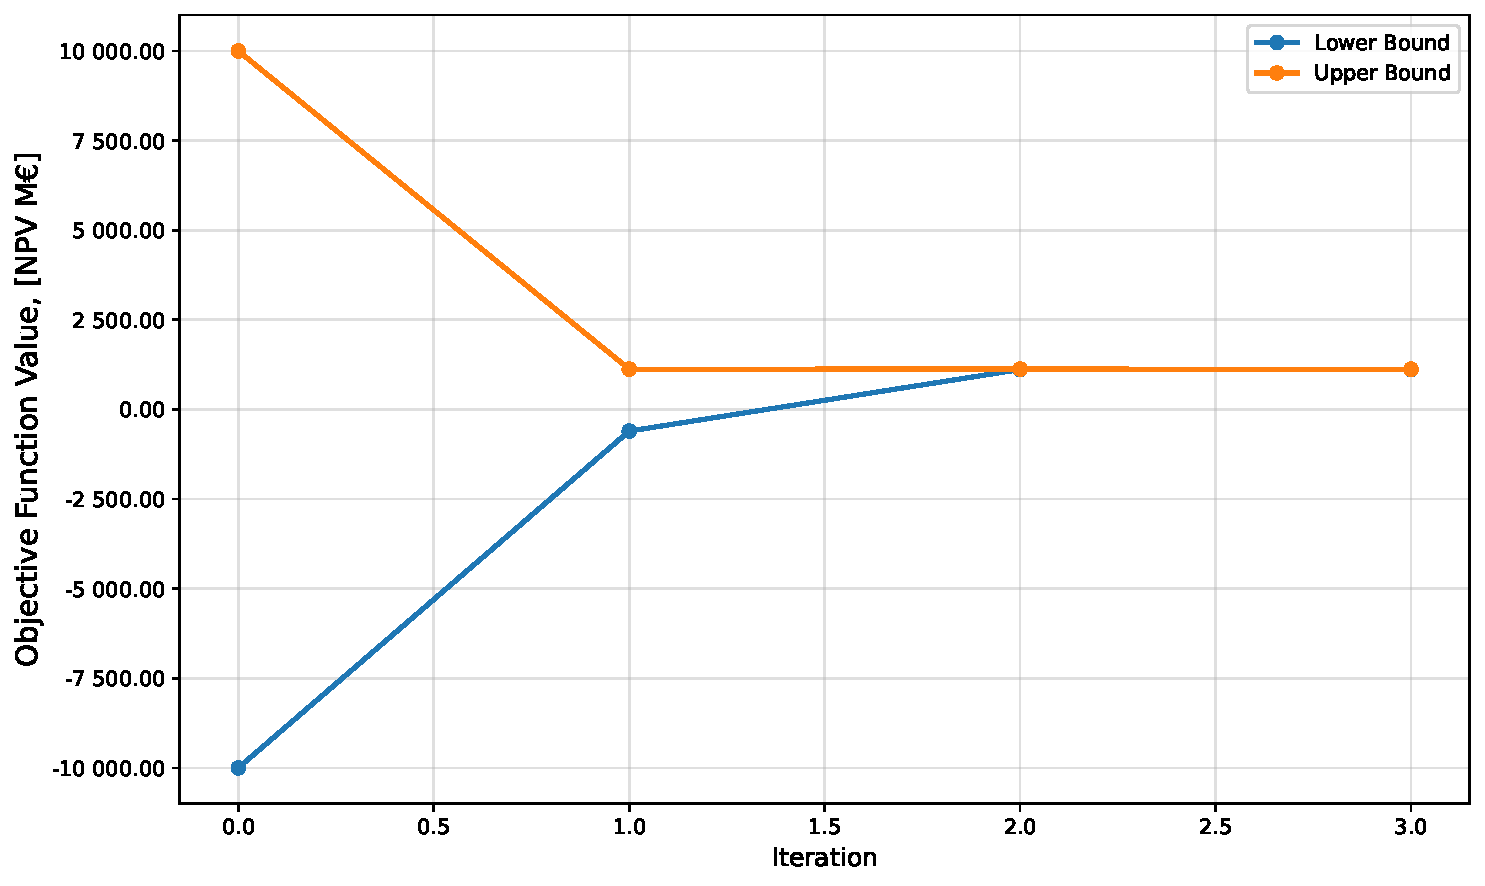
\includegraphics[width=0.90\textwidth]{results_convergence_characteristic.pdf}
    \caption{Convergence of the Benders decomposition algorithm.}
    \label{fig:cs3_results_convergence_characteristic}
\end{figure}

The algorithm converges in four Benders iterations to a relative optimality gap of 0.50\%, with a total runtime of 30\,560~s. 
Although the runtime remains significant, it should be interpreted in light of the dimensionality of the problem, which combines multi-year planning, nonlinear AC-constrained coordinated operation, degradation tracking, and multiple uncertainty scenarios. These results support the practical applicability of the proposed decomposition architecture for off-line planning studies.
The observed performance is enabled by decomposing the planning and operational layers into smaller tractable subproblems. In addition, the formulation naturally supports parallel solution of the operational subproblems, which can further reduce effective wall-clock time in large-scale implementations.

\subsection{Operational Planning Results}
\label{subsec:results_operational_planning}

This subsection summarizes the main operational results and compares them against the two benchmark cases: uncoordinated operation and coordinated operation without shared ESSs.

\subsubsection{Main Results}

Table~\ref{tab:cs3_results_operational_planning_summary} summarizes the main operational outcomes for the three test cases, including total operating cost, RES generation, and RES curtailment for each representative year. All values correspond to daily averages across the four representative days of each year, whereas day-by-day results are reported in Table~\ref{tab:cs3_results_summary_years_days} of~\ref{app:results}. RES curtailment is reported as \textit{apparent energy} (MVAh), because RES generators in the model can provide reactive power support. Accordingly, curtailment is defined with respect to apparent power rather than active power alone. For the coordinated cases, the reported percentage variations are computed relative to the corresponding values of the uncoordinated benchmark.

\begin{table}[htbp!]
    \centering
    \caption{Summary of the main operational planning results.}
    \resizebox{1.00\textwidth}{!}{
        \begin{tabular}{lll ccccc}
            \toprule
            ~ & ~ & ~ & \multicolumn{5}{c}{Year}\\ \cmidrule{4-8}
            \multicolumn{3}{l}{Test Case} & 2025 & 2028 & 2031 & 2034 & 2037\\
            \midrule
            \multicolumn{3}{l}{Uncoordinated}\\ \cmidrule{2-8}
            ~ & \multicolumn{2}{l}{Operational Cost, [\euro]}   & 228\,160.22 & 259\,520.80 & 211\,683.68 & 247\,772.49 & 273\,955.22\\
            ~ & \multicolumn{2}{l}{RES Generation, [MWh]}       & 917.65 & 962.18 & 1\,348.91 & 1\,381.60 & 1\,314.22\\
            ~ & \multicolumn{2}{l}{RES Curtailment, [MVAh]}     & 1.30 & 2.77 & 81.23 & 54.34 & 409.29\\ \midrule
            \multicolumn{3}{l}{Without Shared ESSs}\\ \cmidrule{2-8}
            ~ & \multicolumn{2}{l}{Operational Cost}\\       
            ~ & ~ & Total, [\euro]  & 222\,309.25 & 250\,720.96 & 202\,001.02 & 236\,819.08 & 228\,540.87\\
            ~ & ~ & Variation, [\%] & -2.56\% & -3.39\% & -4.57\% & -4.42\% & -16.58\%\\ \cmidrule{2-8}
            ~ & \multicolumn{2}{l}{RES Generation}\\
            ~ & ~ & Total, [MWh]    & 907.86 & 947.99 & 1\,415.01 & 1\,422.13 & 1\,677.43\\
            ~ & ~ & Variation, [\%] & -1.07\% & -1.47\% & 4.90\% & 2.93\% & 27.64\%\\ \cmidrule{2-8}
            ~ & \multicolumn{2}{l}{RES Curtailment}\\       
            ~ & ~ & Total, [MVAh]   & 12.95 & 17.82 & 15.24 & 13.80 & 46.89\\
            ~ & ~ & Variation, [\%] & 894.07\% & 543.90\% & -81.24\% & -74.60\% & -88.54\% \\ \midrule
            \multicolumn{3}{l}{With Shared ESSs}\\ \cmidrule{2-8}
            ~ & \multicolumn{2}{l}{Operational Cost}\\   
            ~ & ~ & Total, [\euro]  & 222\,393.22 & 249\,768.49 & 202\,309.71 & 239\,441.31 & 223\,948.57\\
            ~ & ~ & Variation, [\%] & -2.53\% & -3.76\% & -4.43\% & -3.36\% & -18.25\%\\ \cmidrule{2-8}
            ~ & \multicolumn{2}{l}{RES Generation}\\       
            ~ & ~ & Total, [MWh]    & 907.86 & 947.97 & 1\,414.95 & 1\,410.36 & 1\,692.24\\
            ~ & ~ & Variation, [\%] & -1.07\% & -1.48\% & 4.90\% & 2.08\% & 28.76\%\\ \cmidrule{2-8}
            ~ & \multicolumn{2}{l}{RES Curtailment}\\       
            ~ & ~ & Total, [MVAh]   & 12.94 & 17.81 & 15.28 & 25.57 & 32.08\\
            ~ & ~ & Variation, [\%] & 893.89\% & 543.59\% & -81.19\% & -52.95\% & -92.16\%\\
            \bottomrule
        \end{tabular}
    }
    \label{tab:cs3_results_operational_planning_summary}
\end{table}

Overall, coordinated operation consistently improves performance relative to uncoordinated operation, and the addition of shared ESSs further enhances these benefits in the later stages of the planning horizon. The strongest differences emerge from 2031 onward, when rising RES penetration increases both system stress and the value of flexibility.
It should be noted, however, that the shared ESS case does not outperform the benchmark without shared ESSs for every metric in every year. This is expected because the shared ESS is scheduled within a coordinated operation framework subject to AC network constraints and degradation-aware intertemporal trade-offs. As a result, the storage asset may in some periods prioritize voltage support, reactive-power provision, or preservation of future usable capacity rather than minimizing curtailment or operating cost in that year alone. The value of shared ESS deployment should therefore be assessed over the full planning horizon rather than through isolated annual indicators.

\subsubsection{Network Constraint Violations Mitigation}
\label{subsubsec:network_violations}

Under uncoordinated operation, voltage magnitude violations appear as early as the first representative year of the planning horizon (2025). As an illustrative example, Figure~\ref{fig:cs3_results_bus_voltage_violation} reports the voltage magnitude profile at TN bus~3 for the winter representative day of 2025, comparing uncoordinated operation with coordinated operation both with and without shared ESSs.

\begin{figure}[htbp]
    \centering
    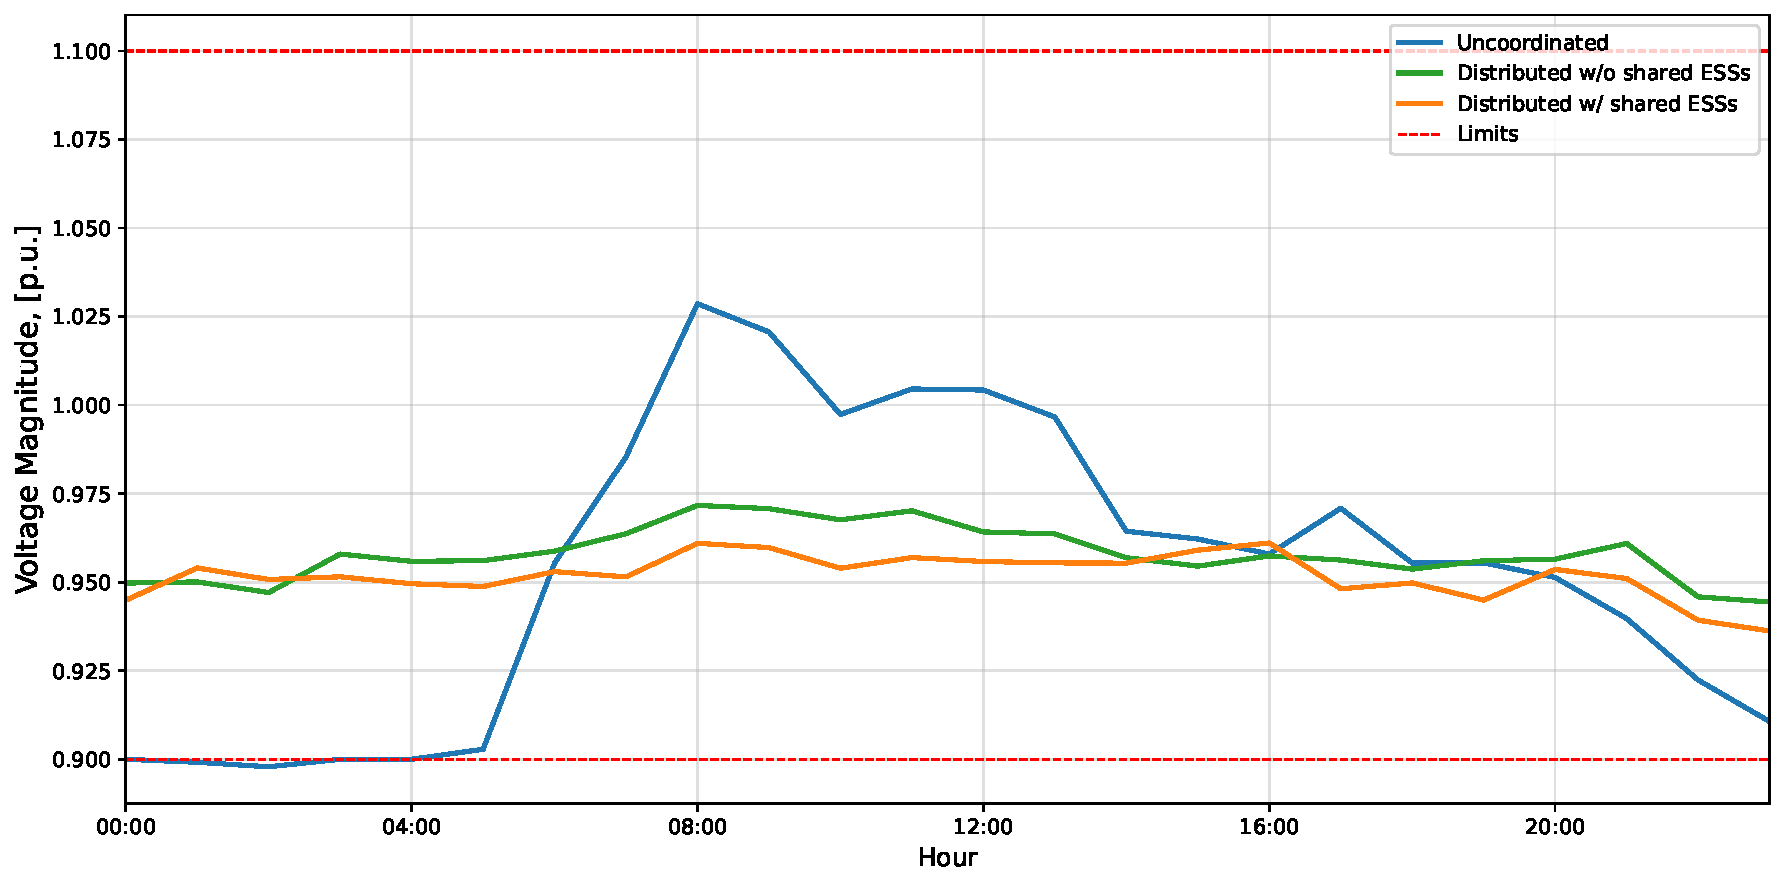
\includegraphics[width=0.95\textwidth]{voltage_profile_node_3_2025_Winter.pdf}
    \caption{Voltage magnitude at TN bus~3 for the winter representative day of 2025 under the three operating configurations.}
    \label{fig:cs3_results_bus_voltage_violation}
\end{figure}

Both coordinated configurations eliminate the voltage violation through system-wide flexibility activation. This suggests that, in the absence of coordination, maintaining compliance with voltage limits would likely require conventional network reinforcement. Coordinated operation therefore emerges as a non-wire alternative capable of mitigating voltage problems without immediate conventional reinforcement. This is particularly relevant in systems with growing DER penetration, where improved operational coordination may defer or reduce the need for traditional grid reinforcements.

% Operational costs
\subsubsection{Operational Costs}

As shown in Table~\ref{tab:cs3_results_operational_planning_summary}, coordinated operation consistently reduces total operating costs relative to uncoordinated operation. The additional benefit of shared ESS deployment becomes more pronounced in the later years of the planning horizon, when higher RES penetration amplifies flexibility needs. By 2037, cost reductions reach 16.58\% under coordination without shared ESSs and 18.25\% when shared ESSs are included, showing that shared storage enhances the economic value of coordinated operation.
Figure~\ref{fig:cs3_results_operational_costs} illustrates the evolution of operational costs by representative year, representative day, and test case, disaggregated into conventional generation and flexibility procurement components.

\begin{figure}[htbp]
    \centering
    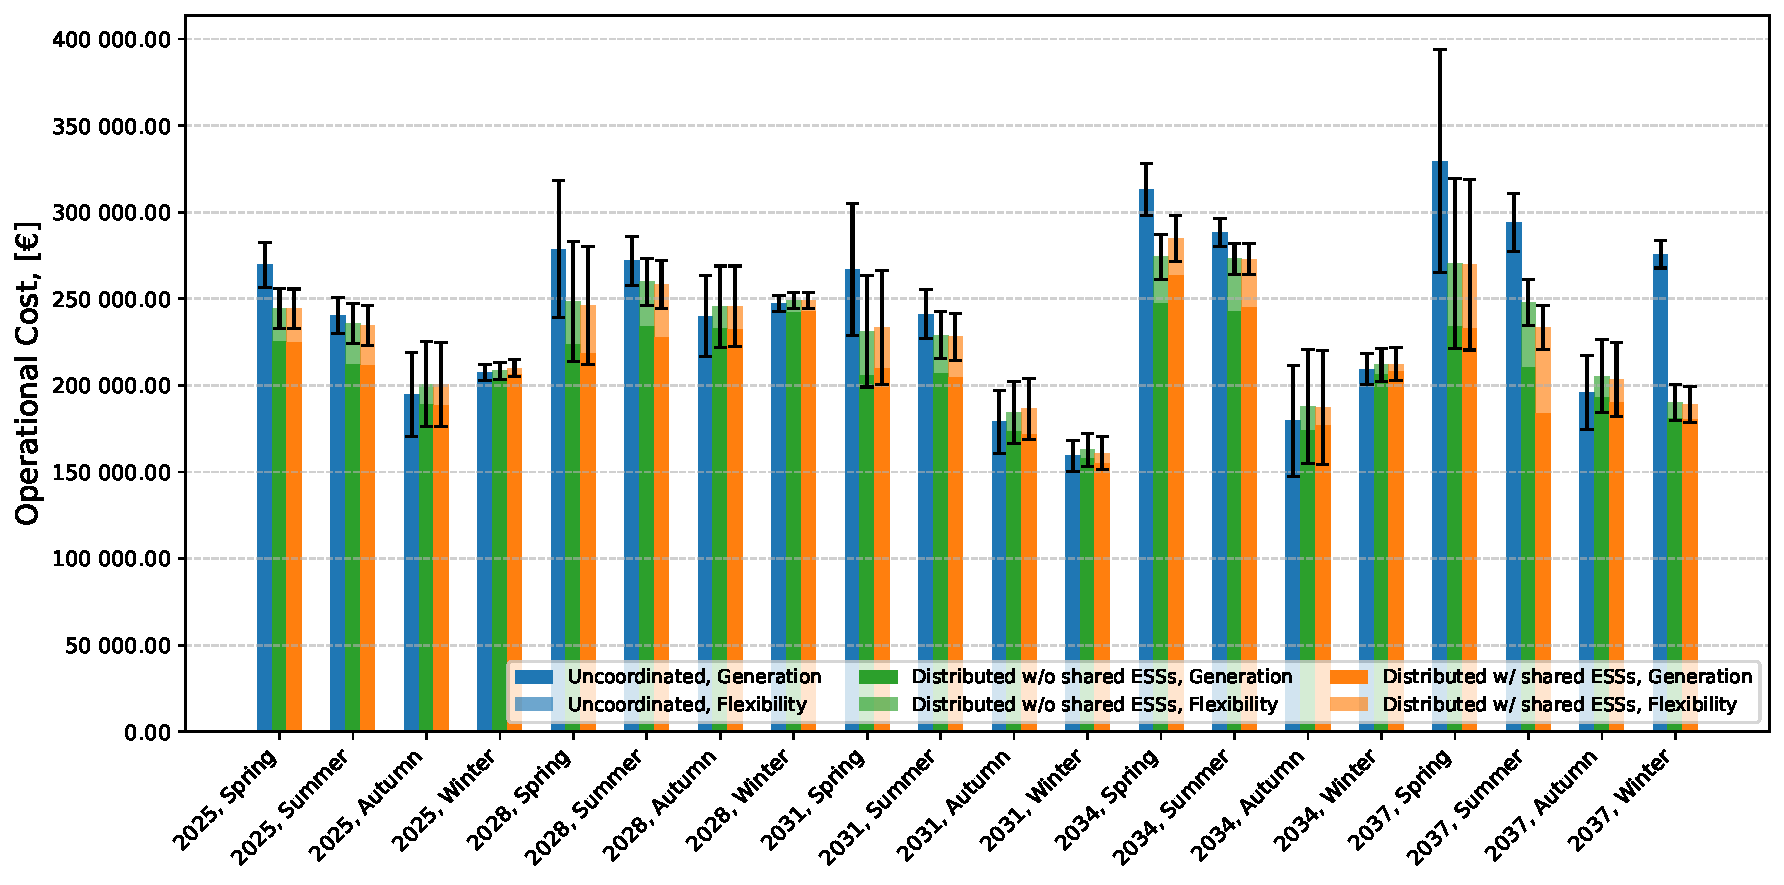
\includegraphics[width=0.95\textwidth]{results_operational_cost_multi_year.pdf}
    \caption{Operational costs by representative year, representative day, and test case.}
    \label{fig:cs3_results_operational_costs}
\end{figure}

Although uncoordinated operation may occasionally yield lower apparent operating costs in isolated representative days during the early years, these outcomes are associated with unresolved technical infeasibilities, notably voltage-limit violations (Subsection~\ref{subsubsec:network_violations}). They should therefore not be interpreted as economically preferable operating points from a system-planning perspective.

% RES generation
\subsubsection{RES Generation}

Table~\ref{tab:cs3_results_operational_planning_summary} shows that the benefits of coordinated operation for renewable integration become substantial from 2031 onward, when rising RES penetration leads to significant curtailment under uncoordinated operation. In 2037, curtailment is reduced by 88.54\% under coordination without shared ESSs and by 92.16\% when shared ESSs are included. 
Figures~\ref{fig:cs3_results_res_generation} and~\ref{fig:cs3_results_res_curtailment} provide a more detailed view of RES generation and curtailment; as noted above, curtailment is reported in MVAh because it is measured with respect to apparent power.

\begin{figure*}[htbp!]
    \centering
    \begin{subfigure}[b]{0.90\textwidth}  
        \centering 
        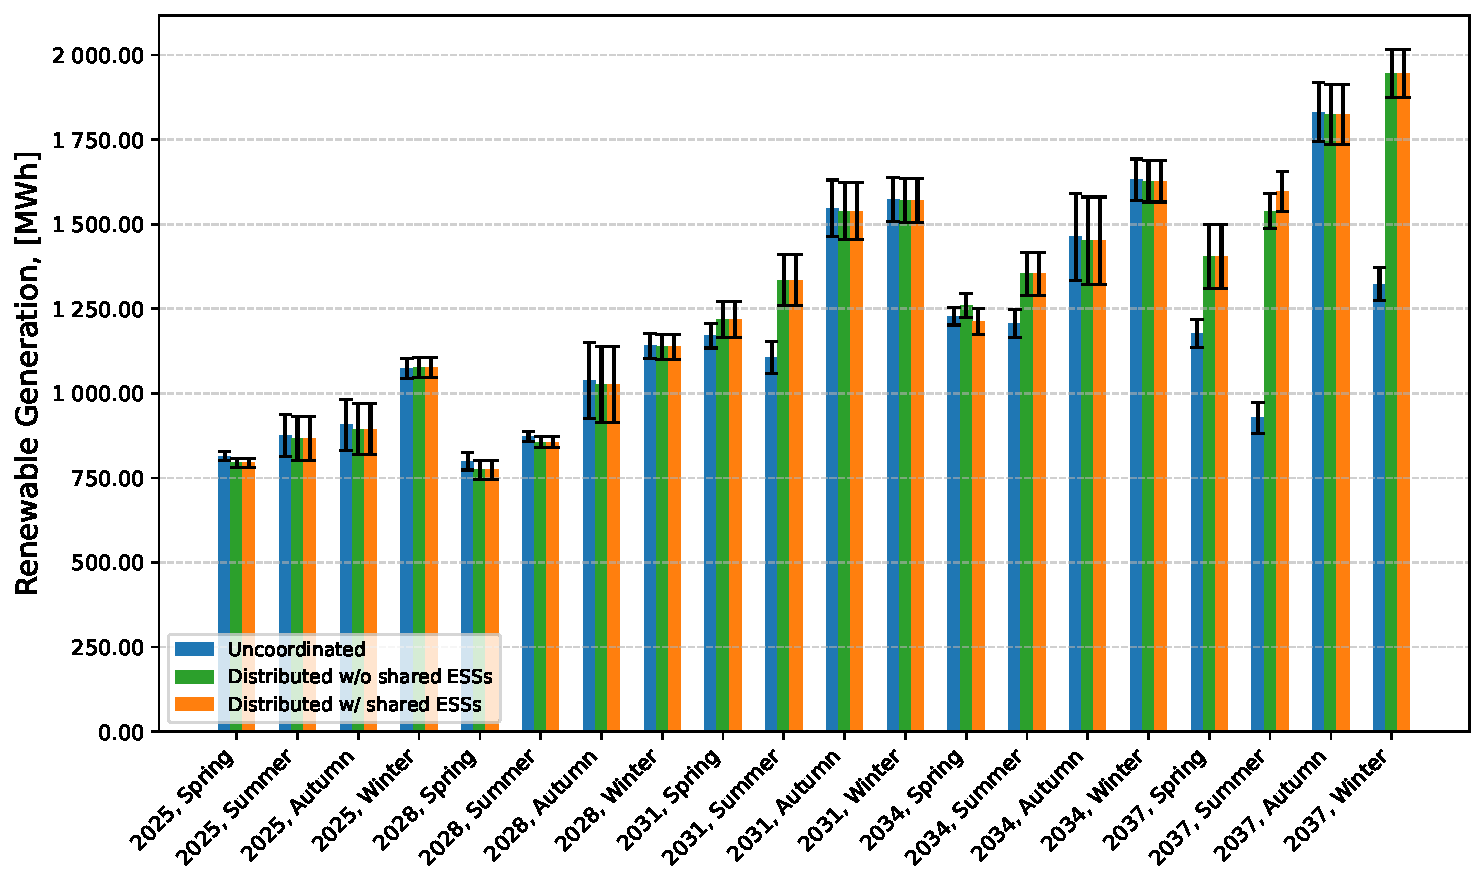
\includegraphics[width=\textwidth]{results_res_generation_active_power_multi_year.pdf}
        \caption{Active energy.}
    \end{subfigure}
    \hfill
    \begin{subfigure}[b]{0.90\textwidth}   
        \centering 
        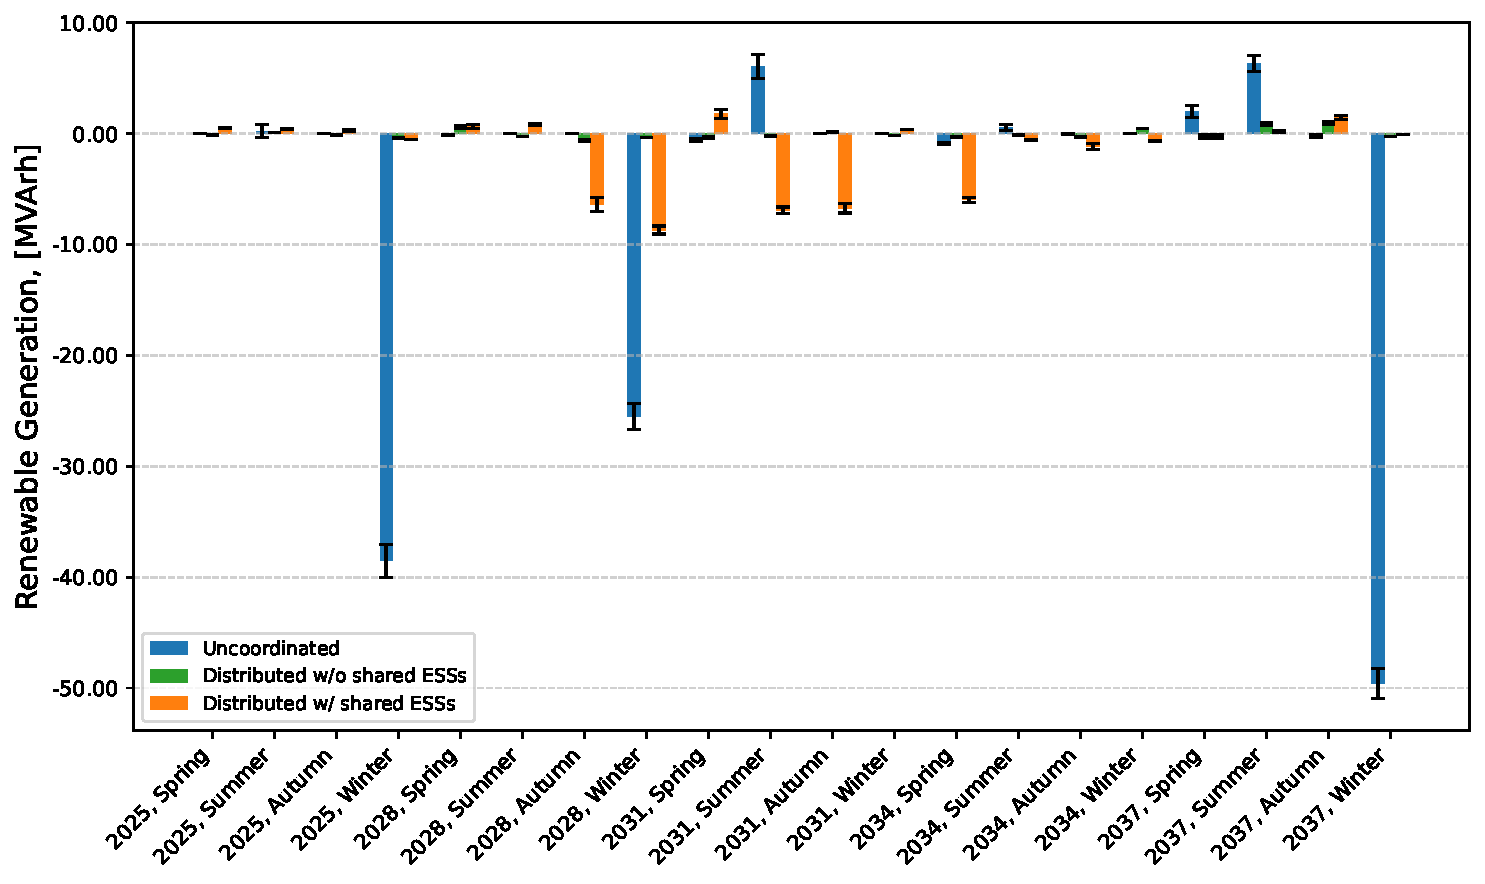
\includegraphics[width=\textwidth]{results_res_generation_reactive_power_multi_year.pdf}
        \caption{Reactive energy.}
        \label{fig:cs3_results_res_generation_reactive}
    \end{subfigure}
    \caption{RES generation by representative year, representative day, and test case.}
    \label{fig:cs3_results_res_generation}
\end{figure*}

\begin{figure}[htbp]
    \centering
    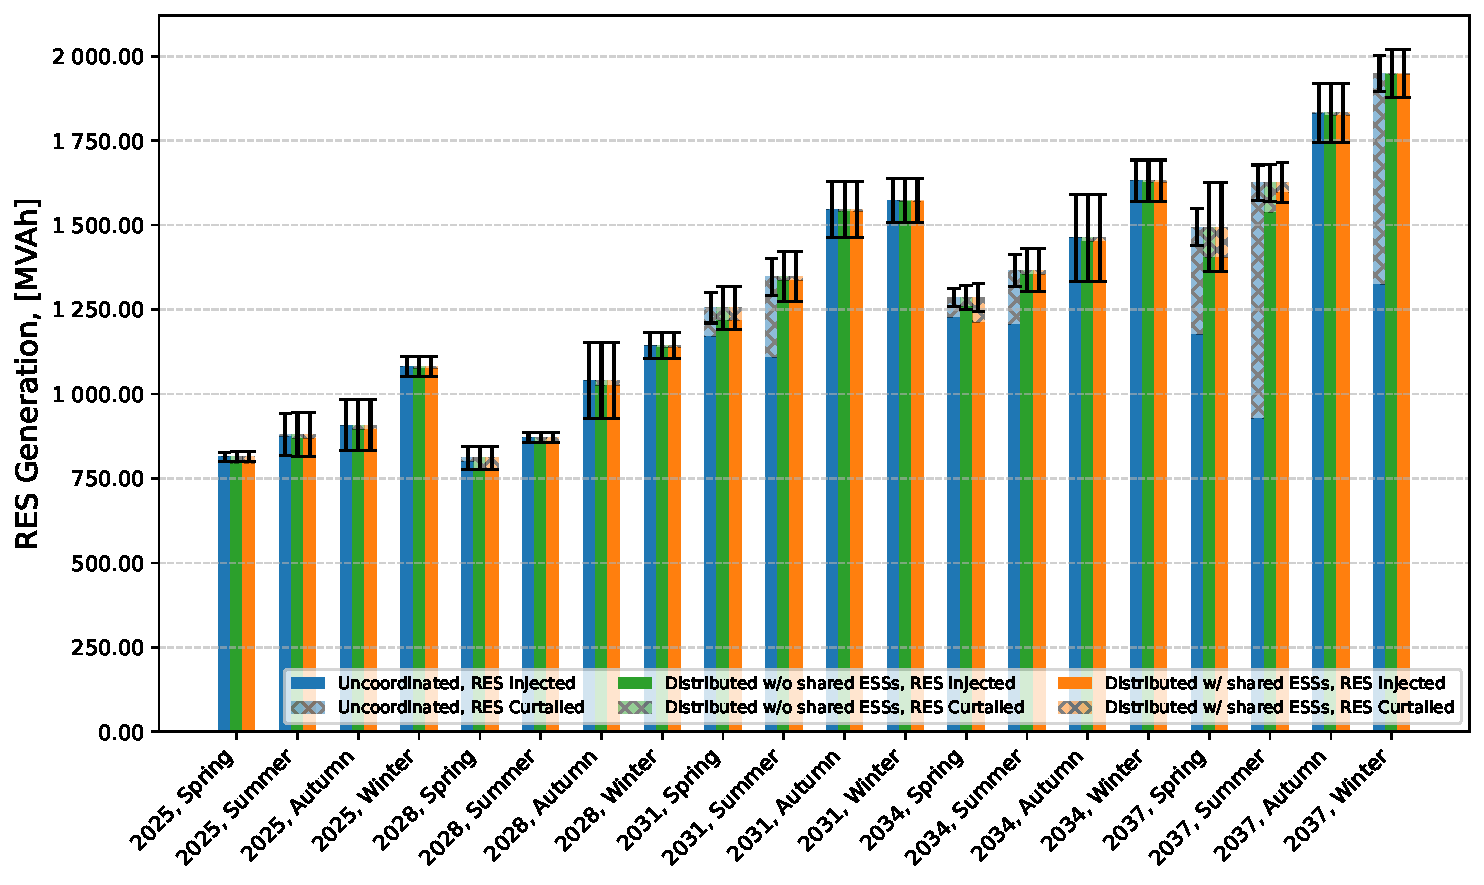
\includegraphics[width=0.90\textwidth]{results_res_generation_curtailment_multi_year.pdf}
    \caption{RES curtailment by representative year, representative day, and test case.}
    \label{fig:cs3_results_res_curtailment}
\end{figure}

Figure~\ref{fig:cs3_results_res_generation_reactive} further highlights the benefits of coordinated operation. Under uncoordinated operation, RES generators absorb large amounts of reactive power in an attempt to support transmission-level voltage regulation, yet these efforts remain insufficient to prevent voltage violations (Figure~\ref{fig:cs3_results_bus_voltage_violation}). By contrast, coordinated operation enables a more efficient allocation of reactive power support, allowing RES generators to operate closer to unitary power factor. This indicates that coordinated flexibility activation becomes increasingly important for sustaining high RES integration as system stress rises over the planning horizon.
This effect also helps explain why the value of shared ESS deployment increases toward the end of the planning horizon: as RES penetration rises, the coupled system requires greater flexibility not only in active power but also in reactive power support and voltage management. Shared ESSs provide an additional controllable resource that can relieve these growing network stresses.

% Flexibility procurement

%\subsubsection{Flexibility Procurement}

%Figure~\ref{fig:cs3_results_flexibility_usage} reports the total flexibility services procurement across representative years, days, and test cases.
%As RES penetration increases over the planning horizon, demand-side flexibility becomes progressively more important, particularly in spring and summer. These results confirm that coordinated operation enables a more effective utilization of existing flexibility resources, aligning flexibility activation with evolving generation patterns and reinforcing the role of ADNs as key contributors to system-wide balancing and voltage support.

%\begin{figure*}[htbp!]
%    \centering
%    \begin{subfigure}[b]{0.90\textwidth}  
%        \centering 
%        \includegraphics[width=\textwidth]{results_flexibility_active_power_multi_year.pdf}
%        \caption{Active energy.}
%    \end{subfigure}
%    \hfill
%    \begin{subfigure}[b]{0.90\textwidth}   
%        \centering 
%        \includegraphics[width=\textwidth]{results_flexibility_reactive_power_multi_year.pdf}
%        \caption{Reactive energy.}
%    \end{subfigure}
%    \caption{Flexibility procurement per representative year and day.} 
%    \label{fig:cs3_results_flexibility_usage}
%\end{figure*}

\subsection{Impact of Planning Horizon Discretization}

Temporal discretization strongly influences degradation modeling accuracy and, consequently, ESS investment decisions. This issue is particularly relevant in storage planning because battery capacity can degrade substantially over relatively short operating horizons.

To assess this effect, two alternative planning configurations are evaluated in addition to the baseline case with a 3-year discretization step:
\begin{itemize}
    \item a 5-year discretization, which reduces temporal resolution while keeping the remaining modeling assumptions unchanged;
    \item a 1-year discretization, which increases temporal resolution to annual intervals. Due to memory limitations, the number of market-price and operational scenarios is reduced to three in each case, while maintaining four representative days per year and three investment scenarios.
\end{itemize}

Consequently, the 1-year discretization case should be interpreted primarily as a sensitivity test on temporal resolution rather than as a perfectly like-for-like comparison with the baseline configuration.

Table~\ref{tab:cs3_shared_ess_investment_plan_5year_discretization} reports the expected shared ESS investment plan obtained under the coarser 5-year discretization. In this case, rather than allocating the entire budget to a single shared ESS at node~7, as in the baseline case, the investment is split between two units installed in 2025: a larger system at node~7, rated at 1.54~MVA/3.09~MWh, and a smaller one at node~9, rated at 0.10~MVA/0.20~MWh. This result illustrates that coarser temporal aggregation can affect both the spatial allocation and sizing of shared ESSs.

\begin{table}[htbp!]
    \centering
    \caption{Shared ESS investment plan for the 5-year discretization case.}
    \centering
    \begin{tabular}{cl ccc}
        \toprule
        Node & Parameter                   & 2025 & 2030 & 2035\\ 
        \midrule
        7 & $S^{\text{Inv}}_{e,y}$, [MVA]  & 1.54  & - & - \\
        ~ & $E^{\text{Inv}}_{e,y}$, [MWh]  & 3.09  & - & - \\
        \midrule
        9 & $S^{\text{Inv}}_{e,y}$, [MVA]  & 0.10  & - & - \\
        ~ & $E^{\text{Inv}}_{e,y}$, [MWh]  & 0.20  & - & - \\
        \midrule
        - & Inv., [NPV M\euro]             & 1.00  & 0.00  & 0.00 \\
        \bottomrule
    \end{tabular}
    \label{tab:cs3_shared_ess_investment_plan_5year_discretization}
\end{table}

Table~\ref{tab:cs3_shared_ess_specs_5year_discretization} reports the expected evolution of energy capacity and SoH of the two installed ESSs. The ESS installed at node~7 reaches an end-of-life SoH of 50.80\%, closely matching the 49.62\% obtained with the 3-year discretization step. By contrast, the ESS installed at node~9 exhibits substantially higher degradation, reflecting more intensive cycling. This result highlights the sensitivity of ESS planning to discretization choices and underscores the importance of accurately capturing degradation effects.

\begin{table}[htbp!]
    \centering
    \caption{Available capacity and SoH of the shared ESSs in the 5-year discretization case.}
    \begin{tabular}{cl ccc}
        \toprule
        Node ID & Parameter & 2025 & 2030 & 2035\\ 
        \midrule
        7 & $E^{\text{Av}}_{e,y}$, [MWh]    & 2.27	    & 1.83	    & 1.57\\
        ~ & SoH, [\%]                       & 73.48\%   & 59.15\%   & 50.80\%\\
        \midrule
        9 & $E^{\text{Av}}_{e,y}$, [MWh]    & 0.13      & 0.10      & 0.07\\ 
        ~ & SoH, [\%]                       & 60.76\%   & 50.91\%   & 38.43\%\\ 
        \bottomrule
    \end{tabular}
    \label{tab:cs3_shared_ess_specs_5year_discretization}
\end{table}

Tables~\ref{tab:cs3_shared_ess_investment_plan_1year_discretization} and~\ref{tab:cs3_shared_ess_specs_1year_discretization} report the investment plan and the evolution of available capacity and SoH, respectively, for the 1-year discretization case. In this case, the investment plan is identical to that obtained in the baseline case: a single shared ESS rated at 1.62~MVA/3.24~MWh is installed at node~7 in 2025.

\begin{table}[htbp!]
    \centering
    \caption{Shared ESS investment plan for the 1-year discretization case.}
    \begin{tabular}{cl ccc c c}
        \toprule
        Node & Parameter                   & 2025 & 2026 & 2027 & \ldots & 2039\\ 
        \midrule
        7 & $S^{\text{Inv}}_{e,y}$, [MVA]  & 1.62  & - & - & \ldots & - \\
        ~ & $E^{\text{Inv}}_{e,y}$, [MWh]  & 3.24  & - & - & \ldots & - \\
        \midrule
        - & Inv., [NPV M\euro]             & 1.00  & 0.00  & 0.00 & \ldots & 0.00 \\
        \bottomrule
    \end{tabular}
    \label{tab:cs3_shared_ess_investment_plan_1year_discretization}
\end{table}

\begin{table}[htbp!]
    \centering
    \caption{Available capacity and SoH of the shared ESS in the 1-year discretization case.}
    \resizebox{1.00\textwidth}{!}{
        \begin{tabular}{l ccc c ccc}
            \toprule
            Parameter & 2025 & 2026 & 2027 & \ldots & 2037 & 2038 &2039\\ 
            \midrule
            $E^{\text{Av}}_{e,y}$, [MWh]    & 3.16	    & 3.07	    & 2.96   & \dots & 2.13     & 2.06    & 1.99 \\
            SoH, [\%]                       & 97.56\%	& 94.56\%	& 91.42\%& \dots & 65.83\%  & 63.65\% & 61.49\%\\
            \bottomrule
        \end{tabular}
    }
    \label{tab:cs3_shared_ess_specs_1year_discretization}
\end{table}

These findings show that temporal discretization can materially influence investment decisions. While coarse discretization reduces computational burden, it may distort degradation dynamics and bias investment outcomes. Conversely, finer discretization improves physical fidelity at the cost of greater computational complexity.

\subsection{Key Insights}

Overall, the results show that the value of shared ESS deployment increases as RES penetration rises and coordinated transmission--distribution operation becomes more important.

The case study yields four main insights:
\begin{enumerate}[(i)]
    \item early shared ESS deployment can be economically attractive under favorable or moderate investment-cost trajectories;
    \item coordinated TSO--DSO operation substantially reduces operating costs and RES curtailment, and these benefits are further enhanced by shared ESS deployment in high-stress operating conditions;
    \item explicitly accounting for degradation prevents overvaluation of shared ESS capacity and leads to more technically credible long-term investment decisions; and
    \item the temporal discretization adopted for the planning horizon materially affects degradation trajectories and can alter both the sizing and spatial allocation of shared ESS investments.
\end{enumerate}

Taken together, these findings confirm that shared ESS planning cannot be reliably addressed through purely static, degradation-neutral, or single-level formulations when storage is expected to provide services across both TN and DNs.


% ====================================================================================================================
%                                                      CONCLUSIONS                                                    
% ====================================================================================================================
\section{Conclusions}
\label{sec:conclusions}

This paper presented a degradation-aware framework for planning shared ESS deployment at TN--DN interface nodes in power systems with high DER penetration. 
The proposed methodology integrates long-term investment planning with short-term coordinated TSO--DSO operation through a bi-level optimization architecture, allowing siting, sizing, and timing decisions to be evaluated under realistic operating conditions and investment uncertainty. 
The upper level is solved by Benders' decomposition, while the operational layer relies on the ADMM-based TSO--DSO coordination framework of~\cite{simoes_2023}, extended here to explicitly represent battery degradation. 

The results show that shared ESSs can provide substantial system-wide benefits when planned and operated within a coordinated TSO--DSO framework. In the case study, coordinated operation with shared ESSs reduces operating costs by up to 18.25\% and RES curtailment by up to 92.16\% relative to uncoordinated operation in the later years of the study horizon, while eliminating the voltage violations observed in the uncoordinated case. These findings indicate that shared ESSs can act as an effective non-wire alternative to conventional network reinforcement when their value is assessed jointly across transmission and distribution levels.

The analysis also highlights the importance of explicitly accounting for degradation in long-term ESS planning. In the case study, the selected ESS is intensively utilized and approaches typical end-of-life SoH thresholds by the end of the study horizon, showing that storage value and storage aging must be assessed jointly. In addition, the sensitivity analysis shows that planning-horizon discretization can materially affect ESS sizing and spatial allocation, reinforcing the need for adequate temporal resolution in degradation-sensitive planning studies.

Future work will focus on extending the framework to additional shared flexibility resources, incorporating richer representations of degradation and uncertainty, and developing tighter approximation and decomposition strategies to improve numerical robustness.

\appendix

% ====================================================================================================================
%                                                        APPENDIX                                                     
% ====================================================================================================================

\section{TSO--DSO Coordinated Operational Planning}
\label{app:admm_updated}

This appendix describes the extensions introduced to the consensus-based ADMM framework proposed in~\cite{simoes_2023} to incorporate the shared ESS degradation subproblem. While the original formulation coordinated TSO and DSO operational planning through consensus on interface variables, the present work introduces an additional shared ESS agent responsible for modeling capacity degradation.
For completeness and reproducibility, the updated algorithm and subproblem formulation are provided below.

\subsection{Updated Algorithm}
\label{app:admm_updated_algorithm}

Algorithm~\ref{alg:operational_planning_degradation} presents the updated pseudo-code of the consensus ADMM-based TSO--DSO coordinated operational planning framework introduced in~\cite{simoes_2023}, extended here to include the shared ESS operation subproblem described in Subsection~\ref{subsec:subproblem}.
The extended coordination scheme preserves the sequential update structure of the original consensus-based ADMM algorithm while introducing a third decision-making entity representing the shared ESS agent. This additional agent enforces consistency between the SOs' requested storage schedules and the physical and degradation constraints of the shared ESS portfolio.

\begin{algorithm}[htbp!]

    % Initialization -- DSOs
    \For{$i \in N^I$}{
        DSO$_i$: Create operational planning model\\
        DSO$_i$: Run warm start (assuming $V_{i,t} = 1.0$ p.u. at the TN–DN interface)\\
        DSO$_i$: Update model to ADMM-compatible version\\
    }

    % Initialization -- TSO
    TSO: Create operational planning model\\
    TSO: Run warm start, initializing $V^{I,0}_{i,t}$, $P^{I,0}_{i,t}$, and $Q^{I,0}_{i,t}$ with forecasted values\\
    TSO: Update model to ADMM-compatible version\\

    % ADMM -- Main Iteration
    ADMM: Set $k = 1$, convergence = False\\
    \While{$k \leq k^{\text{max}}$}{

        % DSOs update
        \textbf{DSO updates:}\\
        \For{$i \in N^I$}{
            DSO$_i$: Set 
            $\hat{V}^{I^k}_{i,t}$, 
            $\hat{P}^{I^k}_{i,t}$, 
            $\hat{Q}^{I^k}_{i,t}$, 
            $\hat{P}^{E^k}_{i,t}$, and 
            $\hat{Q}^{E^k}_{i,t}$ 
            to Shared ESSs' targets\\
            DSO$_i$: Solve local operational planning problem\\
            DSO$_i$: Update dual variables 
            $\pi^{I,V^k}_{i,t}$, 
            $\pi^{I,P^k}_{i,t}$, 
            $\pi^{I,Q^k}_{i,t}$, 
            $\pi^{E,P^k}_{i,t}$, 
            $\pi^{E,Q^k}_{i,t}$\\
        }   

        % Convergence evaluation
        ADMM: Evaluate convergence criteria\\
        \If{converged}{\textbf{exit}}

        % TSO update
        \textbf{TSO update:}\\
        TSO: Set 
        $\hat{V}^{I^k}_{i,t}$, 
        $\hat{P}^{I^k}_{i,t}$, 
        $\hat{Q}^{I^k}_{i,t}$, 
        $\hat{P}^{E^k}_{i,t}$, and 
        $\hat{Q}^{E^k}_{i,t}$
        to DSOs' targets\\
        TSO: Solve operational planning problem\\
        TSO: Update dual variables 
        $\pi^{I,V^k}_{i,t}$, 
        $\pi^{I,P^k}_{i,t}$, 
        $\pi^{I,Q^k}_{i,t}$, 
        $\pi^{E,P^k}_{i,t}$, 
        $\pi^{E,Q^k}_{i,t}$\\

        % Convergence evaluation
        ADMM: Evaluate convergence criteria\\
        \If{converged}{\textbf{exit}}

        % ESS degradation model
        \textbf{Shared ESS operation update:}\\
        Shared ESS: Set 
        $\hat{P}^{E^k}_{i,t}$, and 
        $\hat{Q}^{E^k}_{i,t}$
        to TSO's targets\\
        Shared ESS: Solve operation problem\\
        Shared ESS: Update dual variables 
        $\pi^{E,P^k}_{i,t}$, 
        $\pi^{E,Q^k}_{i,t}$\\

        % Convergence evaluation
        ADMM: Evaluate convergence criteria\\
        \If{converged}{\textbf{exit}}
        
        $k = k + 1$
    }  
    \caption{Updated TSO--DSO coordinated operational planning. Integration of the shared ESS degradation subproblem.}
    \label{alg:operational_planning_degradation}
\end{algorithm}

\subsection{ADMM Implementation}
\label{app:admm_updated_implementation}

Within the consensus-based ADMM structure, the shared ESS subproblem acts as a mediator between TSO and DSO power exchange requests and the physical and degradation limits of the storage systems. 
Its role is to reconcile the active- and reactive-power schedules requested by the SOs with the internal physical limits of the shared ESSs and with the intertemporal degradation dynamics linking representative years.

The generic ADMM formulation of the shared ESS operation subproblem is given by:

\begin{subequations}
    \label{model:admm_sess}
    \begin{align}
    \min~f\left(X\right)
    & + \sum_{e \in E^S} \sum_{y \in Y} \sum_{d \in D} \sum_{t \in T} \mathcal{L}^{E,P} \left(P^{E^k}_{e, y, d, t}, \hat{P}^{E^k}_{e, y, d, t}, \pi^{{E,P}^k}_{e, y, d, t} \right) \\
    & + \sum_{e \in E^S} \sum_{y \in Y} \sum_{d \in D} \sum_{t \in T} \mathcal{L}^{E,Q} \left(Q^{E^k}_{e, y, d, t}, \hat{Q}^{E^k}_{e, y, d, t}, \pi^{{E,Q}^k}_{e, y, d, t} \right) \nonumber\\
    \text{s.t.} \quad & h \left(X, P^{E^k}_{e,t}, Q^{E^k}_{e,t} \right) \leq 0
    \label{eq:admm_sess_cons}
    \end{align}
\end{subequations}

\noindent
where:
\begin{itemize}
    \item Sets and variables:
    \begin{itemize}
        \item $E^S \subseteq E$: set of shared ESSs installed at TN--DN interface nodes.
        \item $Y$: set of representative years in the planning horizon.
        \item $D$: set of representative days.
        \item $T$: set of intra-day time periods.
        \item $K$: set of ADMM iterations.
        \item $X$: vector of local decision variables.
    \end{itemize}
    \item Objective function:
    \begin{itemize}
        \item $f(X)$: local objective function of the shared ESSs subproblem.
    \end{itemize}
    \item Augmented Lagrangian terms:
    \begin{itemize}
        \item $\mathcal{L}^{E,P}$, $\mathcal{L}^{E,Q}$: augmented Lagrangians associated with the shared ESSs' active and reactive power, respectively.
    \end{itemize}
    \item Primal and dual variables:
    \begin{itemize}
        \item $P^{E^k}_{e,y,d,t}$, $Q^{E^k}_{e,y,d,t}$: shared ESS $e \in E^S$ active and reactive power, respectively, in year $y \in Y$, representative day $d \in D$, time instant $t \in T$, and ADMM iteration $k \in K$.
        $\hat{P}^{E^k}_{e,y,d,t}$ and $\hat{Q}^{E^k}_{e,y,d,t}$ denote their local copies representing the counterpart SO requests.
        \item $\pi^{{E,P}^k}_{e,y,d,t}$, $\pi^{{E,Q}^k}_{e,y,d,t}$: dual variables associated with the shared ESS's active and reactive power, respectively, in year $y \in Y$, representative day $d \in D$, in time instant $t \in T$, and ADMM iteration $k \in K$.
    \end{itemize}
    \item Constraints:
    \begin{itemize}
        \item $h(\cdot)$: represents the internal constraints of the shared ESS subproblem.
    \end{itemize}
\end{itemize}

The augmented Lagrangian terms enforcing consensus on shared ESSs' active and reactive power exchanges are defined as follows:

\begin{align}
    \mathcal{L}^{E,P}\left(P^{E^k}_{e,y,d,t}, \hat{P}^{E^k}_{e,y,d,t}, \pi^{{E,P}^k}_{e,y,d,t} \right)
    &= \pi^{{E,P}^k}_{e,y,d,t} \left( \frac{P^{E^k}_{e,y,d,t} - \hat{P}^{E^k}_{e,y,d,t}}{S^\text{Rated}_{e,y}} \right) \\
    &\quad + \frac{\rho^{{E,P}^k}}{2} \left\Vert \frac{P^{E^k}_{e,y,d,t} - \hat{P}^{E^k}_{e,y,d,t}}{S^\text{Rated}_{e,y}} \right\Vert^2
\end{align}

\begin{align}
    \mathcal{L}^{E,Q}\left(Q^{E^k}_{e,y,d,t}, \hat{Q}^{E^k}_{e,y,d,t}, \pi^{{E,Q}^k}_{e,y,d,t} \right)
    &= \pi^{{E,Q}^k}_{e,y,d,t} \left( \frac{Q^{E^k}_{e,y,d,t} - \hat{Q}^{E^k}_{e,y,d,t}}{S^\text{Rated}_{e,y}} \right) \\
    &\quad + \frac{\rho^{{E,Q}^k}}{2} \left\Vert \frac{Q^{E^k}_{e,y,d,t} - \hat{Q}^{E^k}_{e,y,d,t}}{S^\text{Rated}_{e,y}} \right\Vert^2
\end{align}

\noindent
where $\rho^{{E,P}^k}$ and $\rho^{{E,Q}^k}$ are the ADMM penalty parameters associated with the active and reactive power consensus constraints, respectively, at iteration $k \in K$.
These augmented terms jointly penalize deviations between the shared ESS agent's internal power schedules and the reference values communicated by the SOs, effectively steering both parties toward a common solution.

The dual variables are updated at each iteration $k \in K$ according to ($\forall e \in E^S$, $y \in Y$, $d \in D$, $\forall t \in T$, $\forall k \in K$):

\begin{equation}
    \pi^{{E,P}^{k+1}}_{e,y,d,t} :=
    \pi^{{E,P}^{k}}_{e,y,d,t} + 
    \rho^{{E,P}^k} 
    \left(
        P^{E^{k+1}}_{e,y,d,t} - \hat{P}^{E^{k+1}}_{e,y,d,t}
    \right)
\end{equation}

\begin{equation}
    \pi^{{E,Q}^{k+1}}_{e,y,d,t} :=
    \pi^{{E,Q}^{k}}_{e,y,d,t} + 
    \rho^{{E,Q}^k} 
    \left(
        Q^{E^{k+1}}_{e,y,d,t} - \hat{Q}^{E^{k+1}}_{e,y,d,t}
    \right)
\end{equation}

\noindent
where $\pi^{{E,P}^{k}}_{e,y,d,t}$ and $\pi^{{E,Q}^{k}}_{e,y,d,t}$ are coordination multipliers, penalizing mismatches between the shared ESS power outputs and the targets set by the SOs.

The penalty coefficients are updated adaptively to accelerate convergence and improve numerical stability of the algorithm ($\forall k \in K$):

\begin{equation}
    \rho^{{E,P}^{k+1}} := \rho^{{E,P}^{k}} \left( 1 + r^{E,P} \right)
\end{equation}

\begin{equation}
    \rho^{{E,Q}^{k+1}} := \rho^{{E,Q}^{k}} \left( 1 + r^{E,Q} \right)
\end{equation}

\noindent 
where $r^{E,P}$ and $r^{E,Q}$ denote user-defined update rates for the active and reactive power penalties, respectively. 

%Importantly, since no coupling variables or constraints exist between individual ESS units, the formulation is inherently separable across ESS units. This separability improves numerical conditioning, accelerates convergence, and enhances the computational scalability of the framework for large systems with multiple shared storage assets.


\section{Market Data}
\label{app:market_data}

This appendix presents the seasonal wholesale energy and flexibility market price profiles used in the case study. All price trajectories correspond to the base year (2025); annual growth assumptions are given in Section~\ref{sec:case_studies}. 
Figure~\ref{fig:cs3_market_prices} shows the profiles adopted for the summer, autumn, and winter representative days of 2025, respectively. 

\begin{figure*}[htbp]
    \centering
    \subfloat[Spring 2025]{
        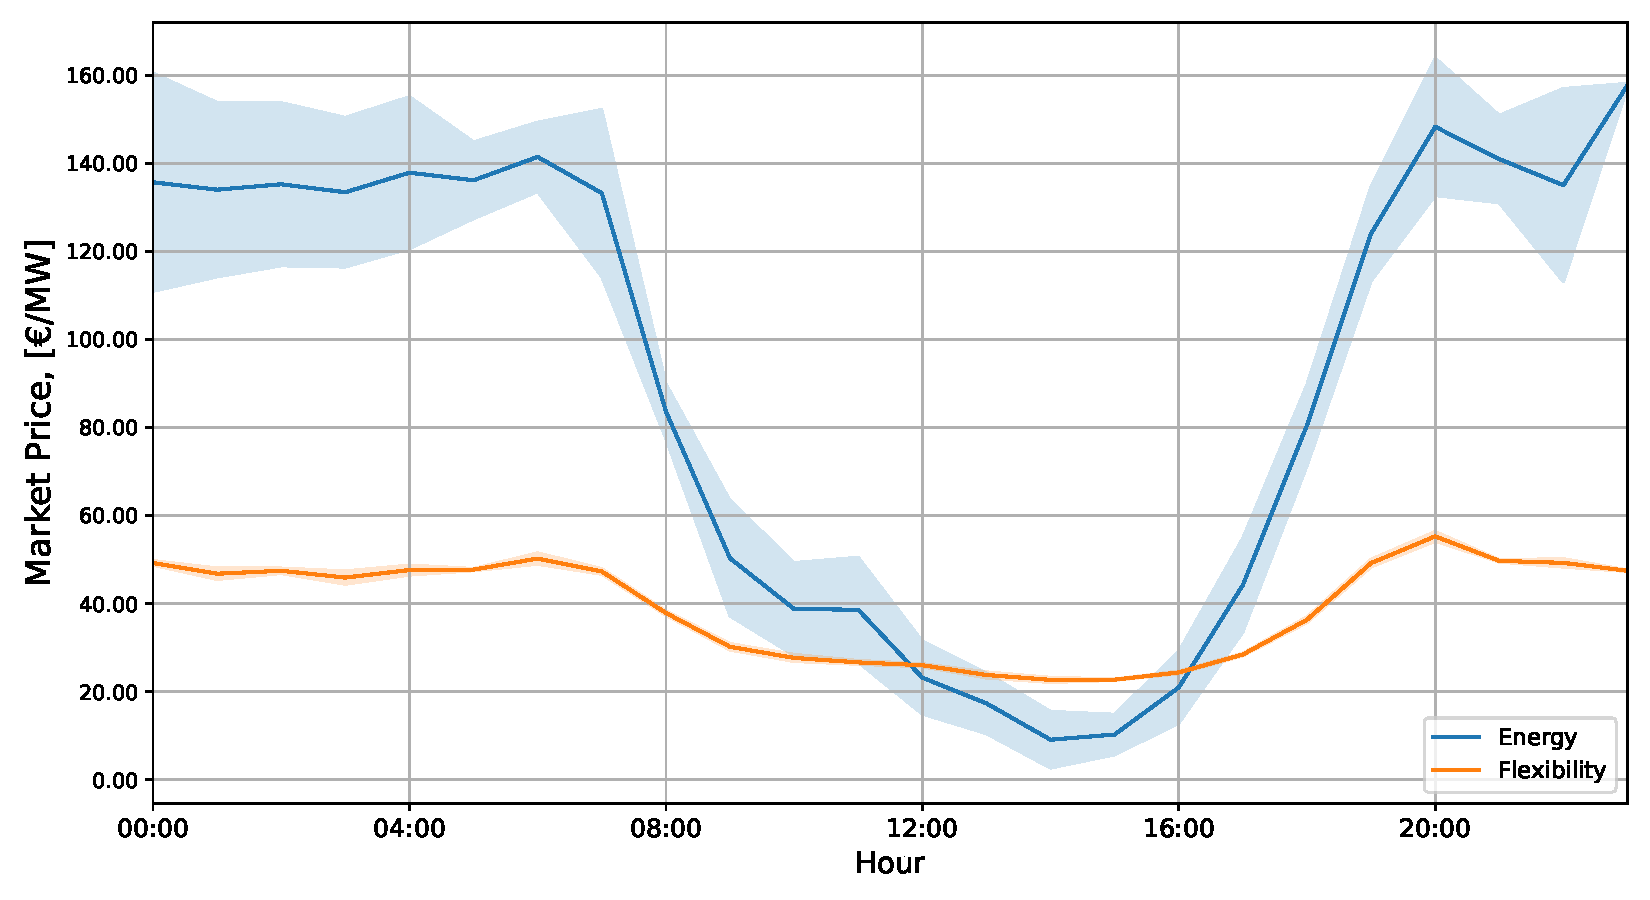
\includegraphics[width=0.475\textwidth]{SRP1_market_prices_2025_Spring.pdf}
    }
    \hfill
    \subfloat[Summer 2025]{
        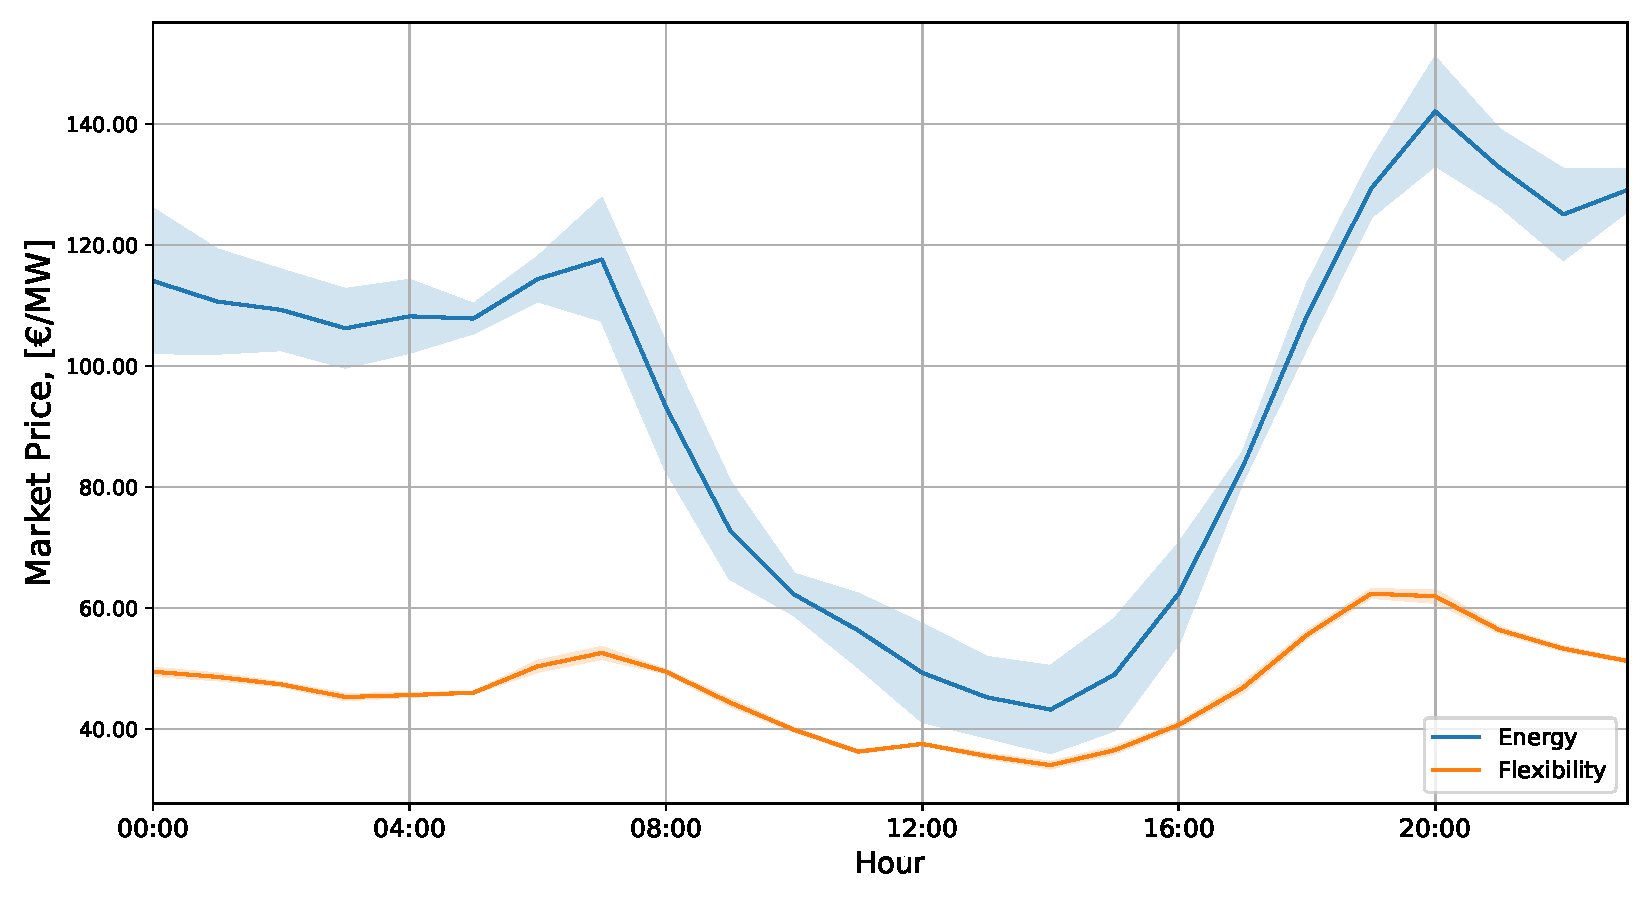
\includegraphics[width=0.475\textwidth]{SRP1_market_prices_2025_Summer.pdf}
    }
    \\[5pt]
    \subfloat[Autumn 2025]{
        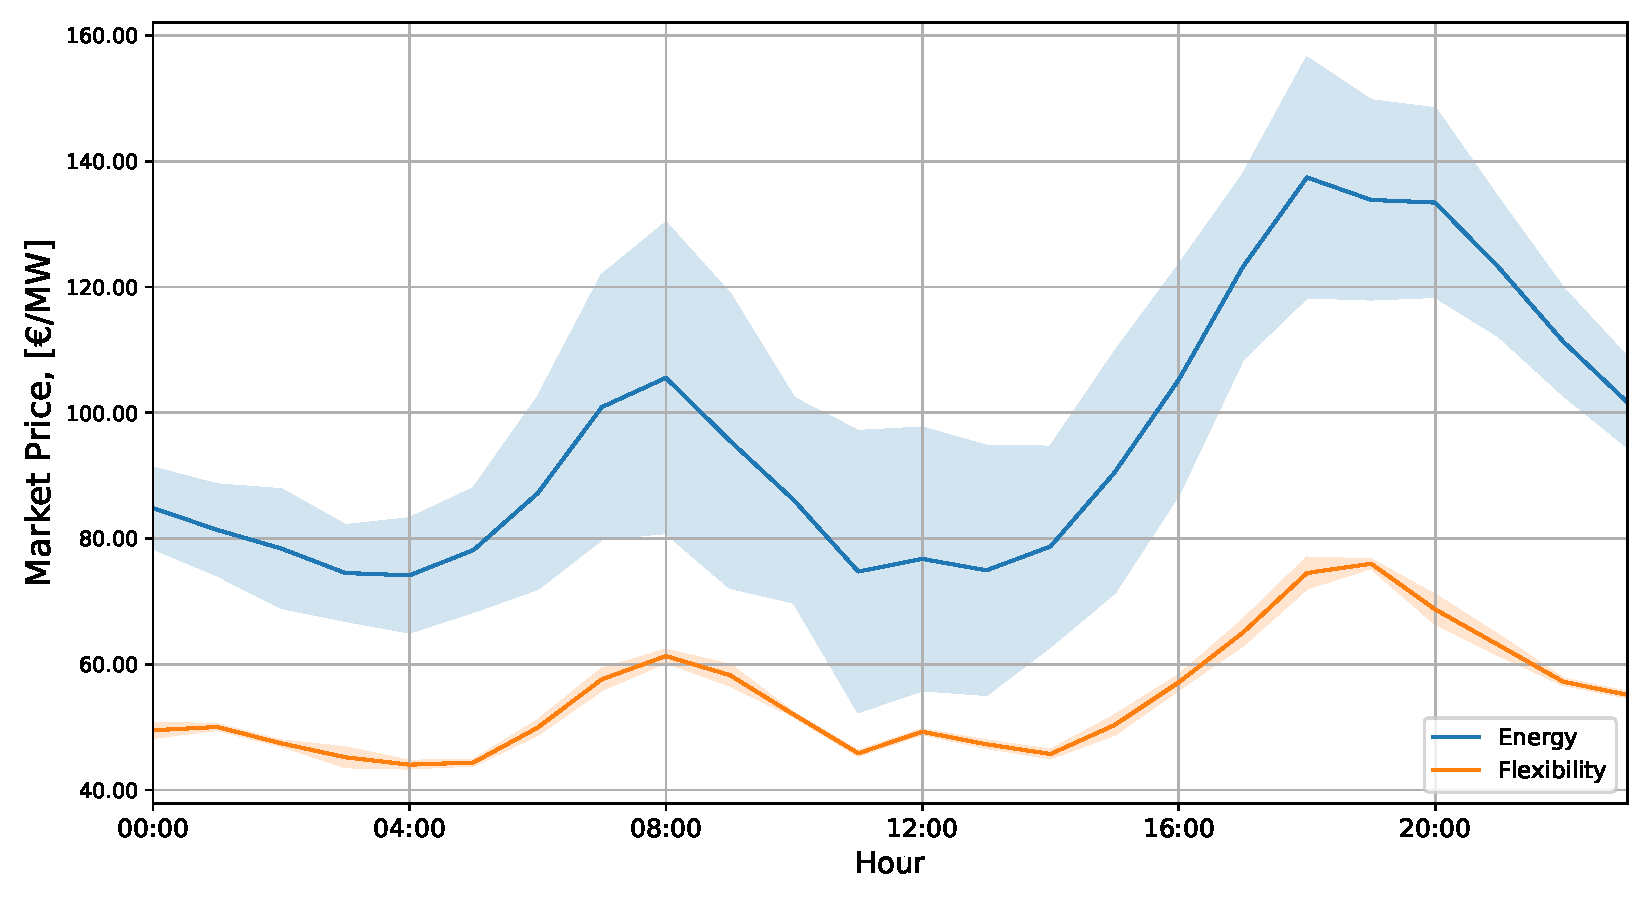
\includegraphics[width=0.475\textwidth]{SRP1_market_prices_2025_Autumn.pdf}
    }
    \hfill
    \subfloat[Winter 2025]{
        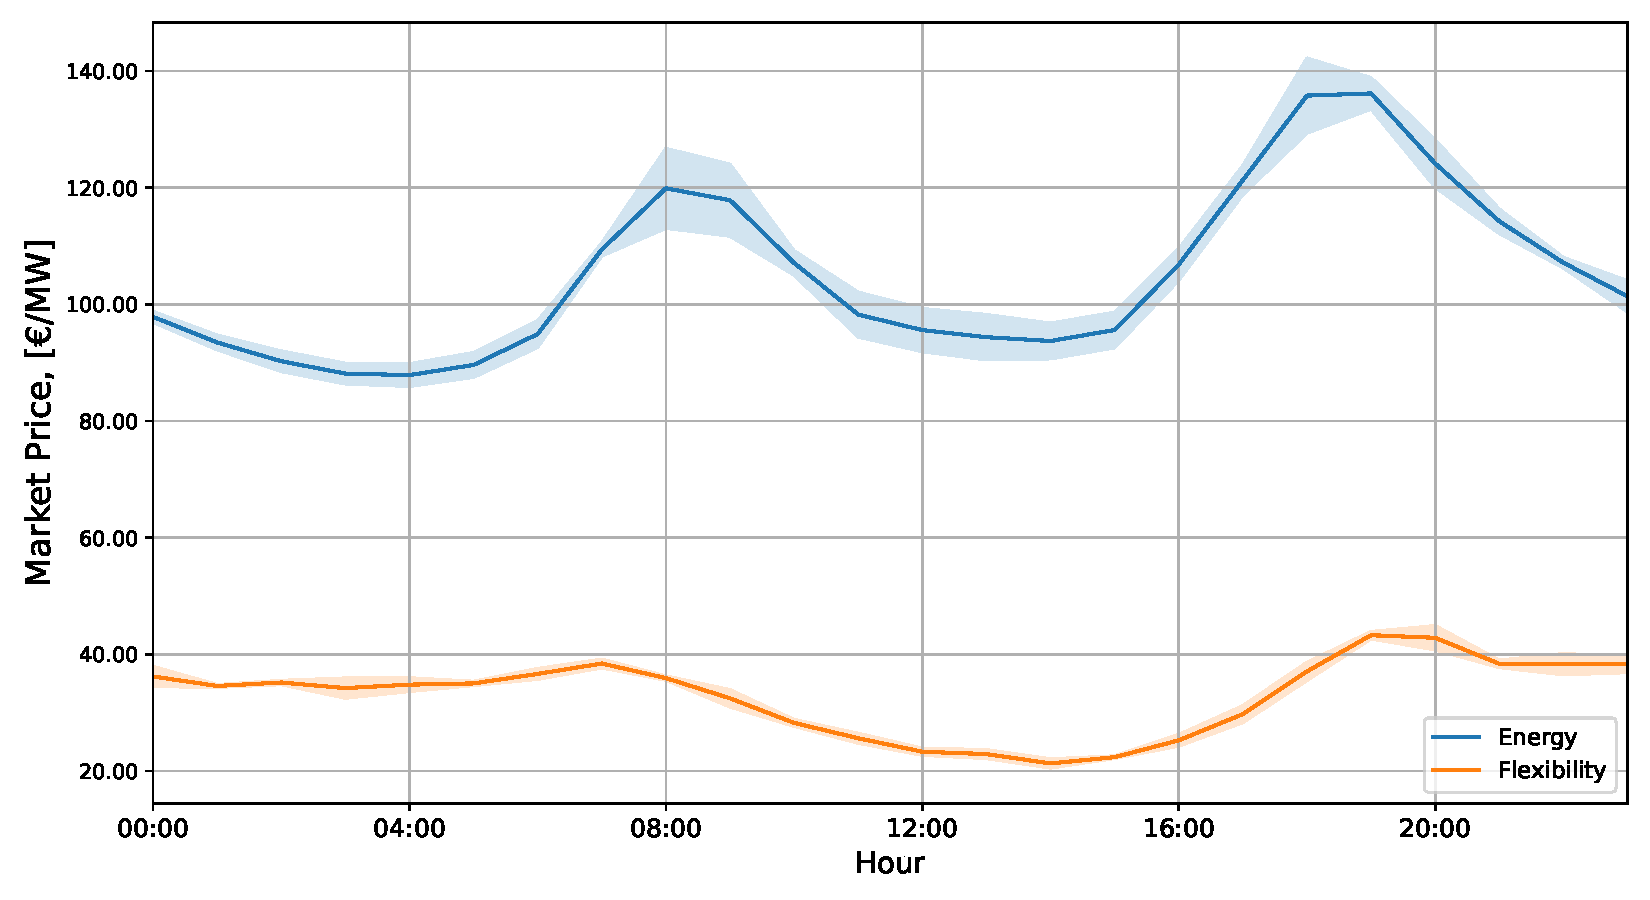
\includegraphics[width=0.475\textwidth]{SRP1_market_prices_2025_Winter.pdf}
    }
    \caption{Wholesale energy and flexibility market prices in 2025.}
    \label{fig:cs3_market_prices}
\end{figure*}

\section{Transmission Network}
\label{app:tn_description}

This appendix presents the RES generation scenarios adopted for the TN in the base planning year (2025). The profiles reflect seasonal variability in wind and solar production and are used as baseline trajectories in all representative years, scaled according to the installed-capacity evolution described in Section~\ref{sec:case_studies}. Figure~\ref{fig:cs3_tn_res_scenarios_2025} shows the RES generation profiles adopted for the spring, summer, autumn, and winter representative days of 2025, respectively.

\begin{figure*}[htbp]
    \centering
    \subfloat[Spring 2025]{
        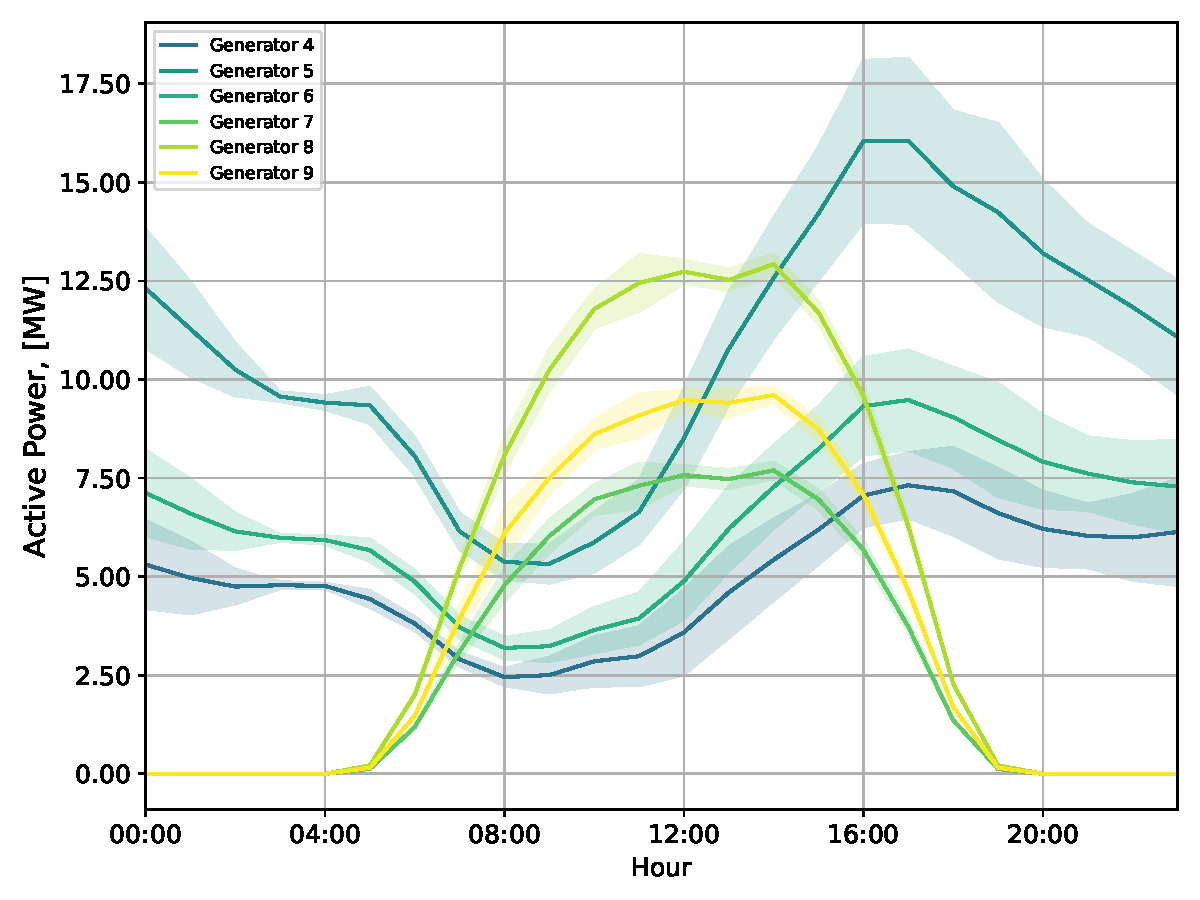
\includegraphics[width=0.475\textwidth]{case9_RES_generation_scenarios_2025_Spring.pdf}
    }
    \hfill
    \subfloat[Summer 2025]{
        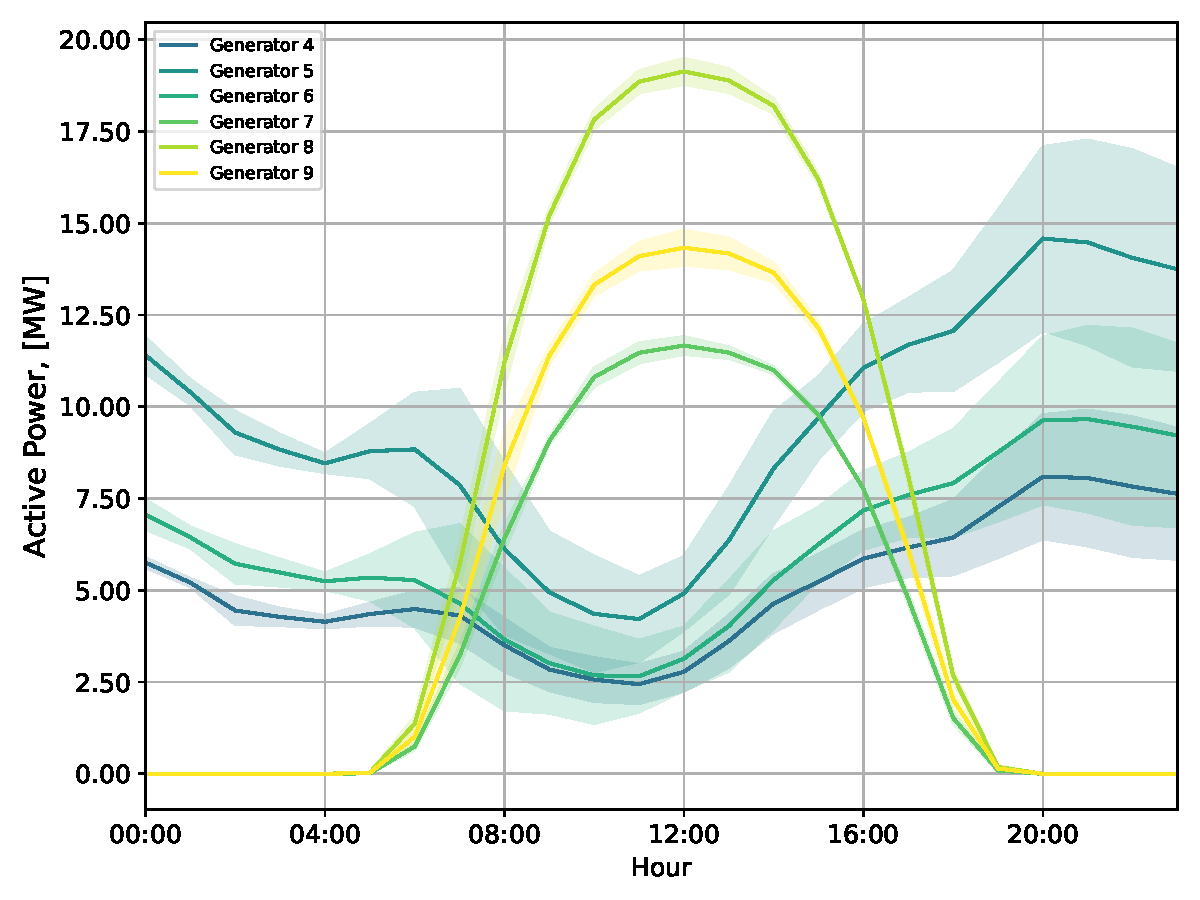
\includegraphics[width=0.475\textwidth]{case9_RES_generation_scenarios_2025_Summer.pdf}
    }
    \\[5pt]
    \subfloat[Autumn 2025]{
        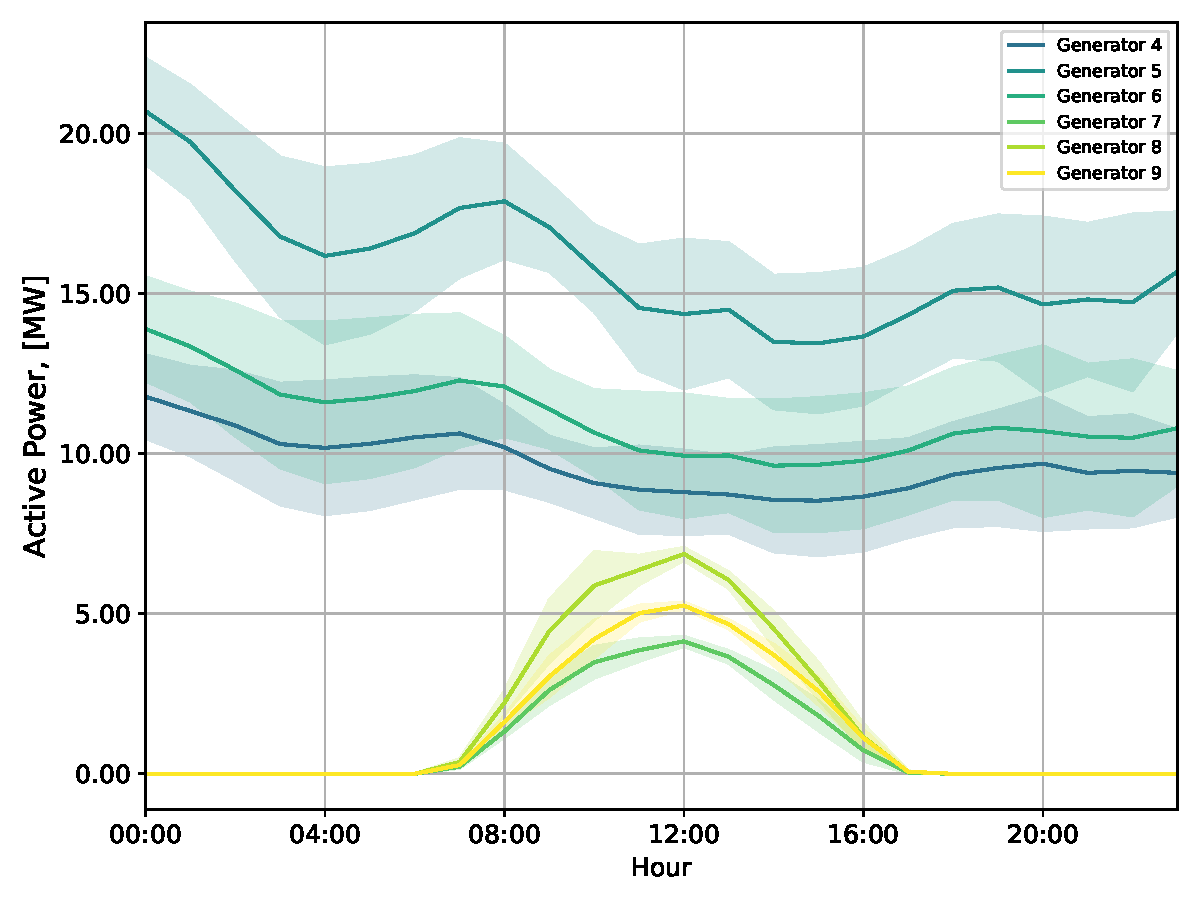
\includegraphics[width=0.475\textwidth]{case9_RES_generation_scenarios_2025_Autumn.pdf}
    }
    \hfill
    \subfloat[Winter 2025]{
        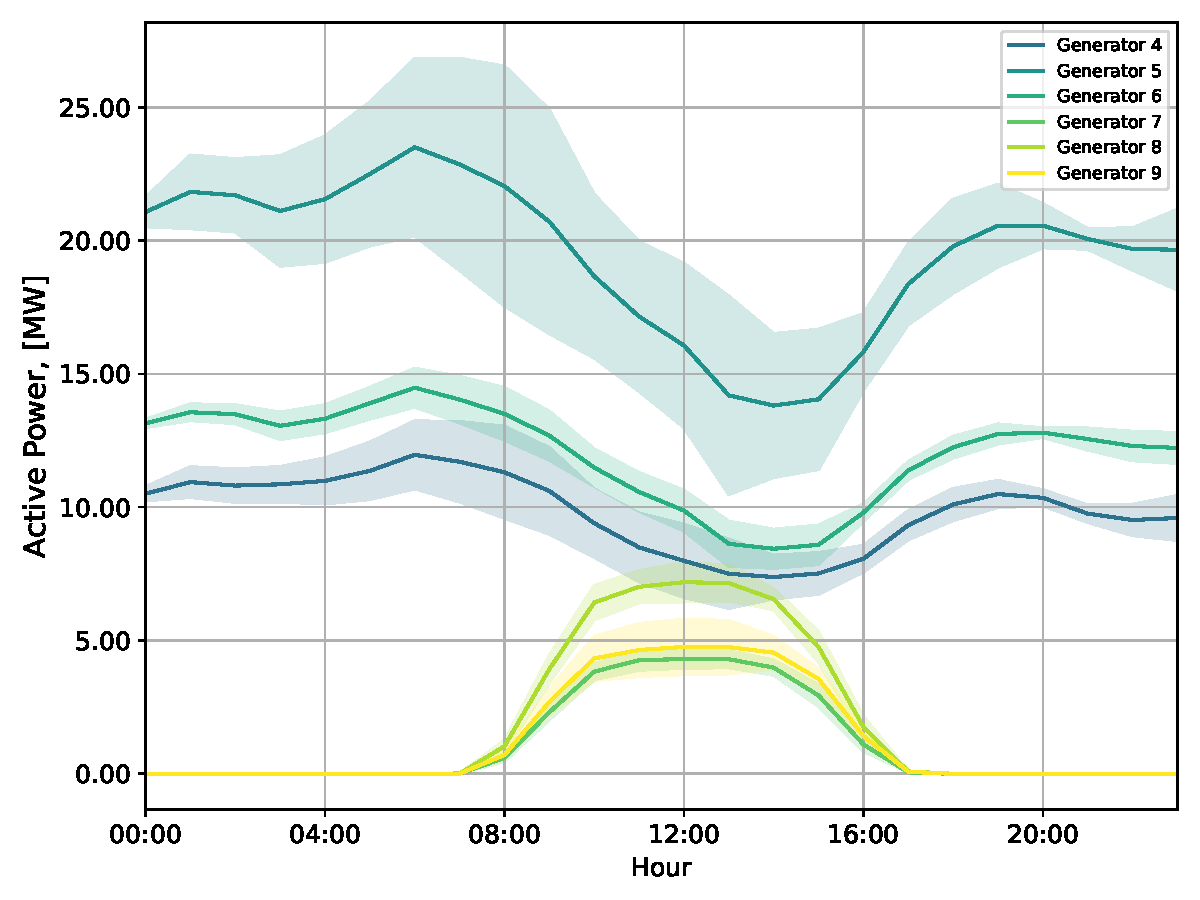
\includegraphics[width=0.475\textwidth]{case9_RES_generation_scenarios_2025_Winter.pdf}
    }
    \caption{TN RES generation profiles for the seasonal scenarios in 2025.}
    \label{fig:cs3_tn_res_scenarios_2025}
\end{figure*}

\section{Distribution Networks}
\label{app:dns_description}

This appendix presents the seasonal RES generation, load, and flexibility profiles adopted for the three ADNs connected to the TN. Although all ADNs share the IEEE 33-bus topology, they differ in installed RES capacities and flexibility penetration, resulting in heterogeneous operating conditions across TN--DN interfaces.
Tables~\ref{tab:cs1_ieee33_buses}--\ref{tab:cs1_ieee33_loads} report the bus, branch, TN connection, and load data common to all ADNs in the case study of Section~\ref{sec:case_studies}. The corresponding RES generator data are given in Tables~\ref{tab:cs3_adn_node_5_res_generators},~\ref{tab:cs3_adn_node_7_res_generators}, and~\ref{tab:cs3_adn_node_9_res_generators} of Subsection~\ref{subsec:case_study_adns}.

\begin{table}[htbp!]
    \centering
    \caption{IEEE 33-bus test system: bus data.}
    \resizebox{1.00\textwidth}{!}{
        \begin{tabular}{ccccccc c ccccccc}
            \cmidrule{1-7} \cmidrule{9-15}
            Bus     & Bus   & $g_{i}$   & $b_{i}$   & $V^\text{Base}_{i}$ & $V^{\text{max}}_i$ & $V^{\text{min}}_i$  & ~ & 
            Bus     & Bus   & $g_{i}$   & $b_{i}$   & $V^\text{Base}_{i}$ & $V^{\text{max}}_i$ & $V^{\text{min}}_i$ \\ 
            \cmidrule{3-7} \cmidrule{9-15}
            ID      & Type  & [p.u.]    & [p.u.]    & [kV]                & [p.u.]             & [p.u.] & ~ &
            ID      & Type  & [p.u.]    & [p.u.]    & [kV]                & [p.u.]             & [p.u.] \\      
            \cmidrule{1-7} \cmidrule{9-15}
            1 & Ref. & 0.00 & 0.00 & 345.00 & 1.10 & 0.90 &  & 18 & PQ & 0.00 & 0.00 & 12.66 & 1.10 & 0.90 \\
            2 & PQ & 0.00 & 0.00 & 12.66 & 1.10 & 0.90 &  & 19 & PQ & 0.00 & 0.00 & 12.66 & 1.10 & 0.90 \\
            3 & PQ & 0.00 & 0.00 & 12.66 & 1.10 & 0.90 &  & 20 & PQ & 0.00 & 0.00 & 12.66 & 1.10 & 0.90 \\
            4 & PQ & 0.00 & 0.00 & 12.66 & 1.10 & 0.90 &  & 21 & PQ & 0.00 & 0.00 & 12.66 & 1.10 & 0.90 \\
            5 & PQ & 0.00 & 0.00 & 12.66 & 1.10 & 0.90 &  & 22 & PQ & 0.00 & 0.00 & 12.66 & 1.10 & 0.90 \\
            6 & PQ & 0.00 & 0.00 & 12.66 & 1.10 & 0.90 &  & 23 & PQ & 0.00 & 0.00 & 12.66 & 1.10 & 0.90 \\
            7 & PQ & 0.00 & 0.00 & 12.66 & 1.10 & 0.90 &  & 24 & PQ & 0.00 & 0.00 & 12.66 & 1.10 & 0.90 \\
            8 & PQ & 0.00 & 0.00 & 12.66 & 1.10 & 0.90 &  & 25 & PQ & 0.00 & 0.00 & 12.66 & 1.10 & 0.90 \\
            9 & PQ & 0.00 & 0.00 & 12.66 & 1.10 & 0.90 &  & 26 & PQ & 0.00 & 0.00 & 12.66 & 1.10 & 0.90 \\
            10 & PQ & 0.00 & 0.00 & 12.66 & 1.10 & 0.90 &  & 27 & PQ & 0.00 & 0.00 & 12.66 & 1.10 & 0.90 \\
            11 & PQ & 0.00 & 0.00 & 12.66 & 1.10 & 0.90 &  & 28 & PQ & 0.00 & 0.00 & 12.66 & 1.10 & 0.90 \\
            12 & PQ & 0.00 & 0.00 & 12.66 & 1.10 & 0.90 &  & 29 & PQ & 0.00 & 0.00 & 12.66 & 1.10 & 0.90 \\
            13 & PQ & 0.00 & 0.00 & 12.66 & 1.10 & 0.90 &  & 30 & PQ & 0.00 & 0.00 & 12.66 & 1.10 & 0.90 \\
            14 & PQ & 0.00 & 0.00 & 12.66 & 1.10 & 0.90 &  & 31 & PQ & 0.00 & 0.00 & 12.66 & 1.10 & 0.90 \\
            15 & PQ & 0.00 & 0.00 & 12.66 & 1.10 & 0.90 &  & 32 & PQ & 0.00 & 0.00 & 12.66 & 1.10 & 0.90 \\
            16 & PQ & 0.00 & 0.00 & 12.66 & 1.10 & 0.90 &  & 33 & PQ & 0.00 & 0.00 & 12.66 & 1.10 & 0.90 \\
            17 & PQ & 0.00 & 0.00 & 12.66 & 1.10 & 0.90 \\
            \cmidrule{1-7} \cmidrule{9-15}
        \end{tabular}
    }
    \label{tab:cs1_ieee33_buses}
\end{table}

\begin{table}[htbp!]
    \centering
    \caption{IEEE 33-bus test system: branch data.}
    \resizebox{1.00\textwidth}{!}{
        \begin{tabular}{ccccccc c ccccccc}
            \cmidrule{1-7} \cmidrule{9-15}
            Branch  & From    & To      & $r_{ij}$  & $x_{ij}$  & $b^\text{Sh}_{ij}$    & $S^\text{Rated}_{ij}$ & & 
            Branch  & From    & To      & $r_{ij}$  & $x_{ij}$  & $b^\text{Sh}_{ij}$    & $S^\text{Rated}_{ij}$ \\ 
            \cmidrule{4-7} \cmidrule{12-15}
            ID      & Bus ID  & Bus ID  & [p.u.]    & [p.u.]    & [p.u.]                & [MVA] & &
            ID      & Bus ID  & Bus ID  & [p.u.]    & [p.u.]    & [p.u.]                & [MVA] \\      
            \cmidrule{1-7} \cmidrule{9-15}
            1 & 1 & 2 & 0.005753 & 0.002932 & 0.00 & 200.00 &  & 42 & 6 & 7 & 0.011680 & 0.038608 & 0.00 & 75.00\\
            2 & 2 & 3 & 0.030760 & 0.015667 & 0.00 & 150.00 &  & 43 & 7 & 8 & 0.044386 & 0.014668 & 0.00 & 60.00\\
            3 & 3 & 4 & 0.022836 & 0.011630 & 0.00 & 150.00 &  & 44 & 8 & 9 & 0.064264 & 0.046170 & 0.00 & 40.00\\
            4 & 4 & 5 & 0.023778 & 0.012110 & 0.00 & 125.00 &  & 45 & 9 & 10 & 0.065138 & 0.046170 & 0.00 & 40.00\\
            5 & 5 & 6 & 0.051099 & 0.044112 & 0.00 & 125.00 &  & 46 & 10 & 11 & 0.012266 & 0.004056 & 0.00 & 40.00\\
            6 & 6 & 7 & 0.011680 & 0.038608 & 0.00 & 100.00 &  & 47 & 11 & 12 & 0.023360 & 0.007724 & 0.00 & 40.00\\
            7 & 7 & 8 & 0.044386 & 0.014668 & 0.00 & 75.00 &  & 48 & 12 & 13 & 0.091592 & 0.072063 & 0.00 & 30.00\\
            8 & 8 & 9 & 0.064264 & 0.046170 & 0.00 & 75.00 &  & 49 & 13 & 14 & 0.033792 & 0.044480 & 0.00 & 25.00\\
            9 & 9 & 10 & 0.065138 & 0.046170 & 0.00 & 50.00 &  & 50 & 14 & 15 & 0.036874 & 0.032818 & 0.00 & 15.00\\
            10 & 10 & 11 & 0.012266 & 0.004056 & 0.00 & 50.00 &  & 51 & 15 & 16 & 0.046564 & 0.034004 & 0.00 & 10.00\\
            11 & 11 & 12 & 0.023360 & 0.007724 & 0.00 & 50.00 &  & 52 & 16 & 17 & 0.080424 & 0.107378 & 0.00 & 5.00\\
            12 & 12 & 13 & 0.091592 & 0.072063 & 0.00 & 50.00 &  & 53 & 17 & 18 & 0.045671 & 0.035813 & 0.00 & 5.00\\
            13 & 13 & 14 & 0.033792 & 0.044480 & 0.00 & 40.00 &  & 54 & 6 & 26 & 0.012666 & 0.006451 & 0.00 & 50.00\\
            14 & 14 & 15 & 0.036874 & 0.032818 & 0.00 & 40.00 &  & 55 & 26 & 27 & 0.017732 & 0.009028 & 0.00 & 50.00\\
            15 & 15 & 16 & 0.046564 & 0.034004 & 0.00 & 40.00 &  & 56 & 27 & 28 & 0.066074 & 0.058256 & 0.00 & 50.00\\
            16 & 16 & 17 & 0.080424 & 0.107378 & 0.00 & 40.00 &  & 57 & 28 & 29 & 0.050176 & 0.043712 & 0.00 & 50.00\\
            17 & 17 & 18 & 0.045671 & 0.035813 & 0.00 & 40.00 &  & 58 & 29 & 30 & 0.031664 & 0.016128 & 0.00 & 50.00\\
            18 & 2 & 19 & 0.010232 & 0.009764 & 0.00 & 50.00 &  & 59 & 30 & 31 & 0.060795 & 0.060084 & 0.00 & 25.00\\
            19 & 19 & 20 & 0.093851 & 0.084567 & 0.00 & 40.00 &  & 60 & 31 & 32 & 0.019373 & 0.022580 & 0.00 & 25.00\\
            20 & 20 & 21 & 0.025550 & 0.029849 & 0.00 & 40.00 &  & 61 & 32 & 33 & 0.021276 & 0.033081 & 0.00 & 15.00\\
            21 & 21 & 22 & 0.044230 & 0.058481 & 0.00 & 40.00 &  & 62 & 21 & 8 & 0.124785 & 0.124785 & 0.00 & 3.00\\
            22 & 3 & 23 & 0.028152 & 0.019236 & 0.00 & 75.00 &  & 63 & 9 & 15 & 0.124785 & 0.124785 & 0.00 & 3.00\\
            23 & 23 & 24 & 0.056028 & 0.044243 & 0.00 & 60.00 &  & 64 & 12 & 22 & 0.124785 & 0.124785 & 0.00 & 3.00\\
            24 & 24 & 25 & 0.055904 & 0.043743 & 0.00 & 50.00 &  & 65 & 18 & 33 & 0.031196 & 0.031196 & 0.00 & 3.00\\
            25 & 6 & 26 & 0.012666 & 0.006451 & 0.00 & 100.00 &  & 66 & 25 & 29 & 0.031196 & 0.031196 & 0.00 & 3.00\\
            26 & 26 & 27 & 0.017732 & 0.009028 & 0.00 & 100.00 &  & 67 & 2 & 3 & 0.030760 & 0.015667 & 0.00 & 125.00\\
            27 & 27 & 28 & 0.066074 & 0.058256 & 0.00 & 75.00 &  & 68 & 3 & 4 & 0.022836 & 0.011630 & 0.00 & 100.00\\
            28 & 28 & 29 & 0.050176 & 0.043712 & 0.00 & 75.00 &  & 69 & 4 & 5 & 0.023778 & 0.012110 & 0.00 & 100.00\\
            29 & 29 & 30 & 0.031664 & 0.016128 & 0.00 & 75.00 &  & 70 & 5 & 6 & 0.051099 & 0.044112 & 0.00 & 100.00\\
            30 & 30 & 31 & 0.060795 & 0.060084 & 0.00 & 50.00 &  & 71 & 6 & 7 & 0.011680 & 0.038608 & 0.00 & 75.00\\
            31 & 31 & 32 & 0.019373 & 0.022580 & 0.00 & 50.00 &  & 72 & 7 & 8 & 0.044386 & 0.014668 & 0.00 & 60.00\\
            32 & 32 & 33 & 0.021276 & 0.033081 & 0.00 & 50.00 &  & 73 & 8 & 9 & 0.064264 & 0.046170 & 0.00 & 40.00\\
            33 & 21 & 8 & 0.124785 & 0.124785 & 0.00 & 3.00 &  & 74 & 9 & 10 & 0.065138 & 0.046170 & 0.00 & 40.00\\
            34 & 9 & 15 & 0.124785 & 0.124785 & 0.00 & 3.00 &  & 75 & 10 & 11 & 0.012266 & 0.004056 & 0.00 & 40.00\\
            35 & 12 & 22 & 0.124785 & 0.124785 & 0.00 & 3.00 &  & 76 & 11 & 12 & 0.023360 & 0.007724 & 0.00 & 40.00\\
            36 & 18 & 33 & 0.031196 & 0.031196 & 0.00 & 3.00 &  & 77 & 12 & 13 & 0.091592 & 0.072063 & 0.00 & 30.00\\
            37 & 25 & 29 & 0.031196 & 0.031196 & 0.00 & 3.00 &  & 78 & 13 & 14 & 0.033792 & 0.044480 & 0.00 & 25.00\\
            38 & 2 & 3 & 0.030760 & 0.015667 & 0.00 & 125.00 &  & 79 & 14 & 15 & 0.036874 & 0.032818 & 0.00 & 15.00\\
            39 & 3 & 4 & 0.022836 & 0.011630 & 0.00 & 100.00 &  & 80 & 15 & 16 & 0.046564 & 0.034004 & 0.00 & 10.00\\
            40 & 4 & 5 & 0.023778 & 0.012110 & 0.00 & 100.00 &  & 81 & 16 & 17 & 0.080424 & 0.107378 & 0.00 & 5.00\\
            41 & 5 & 6 & 0.051099 & 0.044112 & 0.00 & 100.00 &  & 82 & 17 & 18 & 0.045671 & 0.035813 & 0.00 & 5.00\\
            \cmidrule{1-7} \cmidrule{9-15}
        \end{tabular}
    }
    \label{tab:cs1_ieee33_branches}
\end{table}

\begin{table}[htbp!]
    \centering
    \caption{IEEE 33-bus test system: TN connection data.}
    %\resizebox{1.00\textwidth}{!}{
        \begin{tabular}{ccccccc}
            \toprule
            Generator   & Node  & $P^{G,\text{max}}_{g}$ & $P^{G,\text{min}}_{g}$ & $Q^{G,\text{max}}_{g}$ & $Q^{G,\text{min}}_{g}$ & $V^S_g$ \\ \cmidrule{3-7}
            ID          & ID    & [MW]                   & [MW]                   & [MVAr]                 & [MVAr]                 & [p.u.]\\
            \midrule
            1 & 1 & 250.00 & -250.00 & 250.00 & -250.00 & 1.00\\
            \bottomrule
        \end{tabular}
    %}
    \label{tab:cs1_ieee33_generators}
\end{table}

\begin{table}[htbp!]
    \centering
    \caption{IEEE 33-bus test system: load data.}
    \resizebox{0.85\textwidth}{!}{
        \begin{tabular}{ccc c ccc c ccc}
            \cmidrule{1-3} \cmidrule{5-7} \cmidrule{9-11}
            Load    & Bus   & FL Ratio & ~ & 
            Load    & Bus   & FL Ratio & ~ &
            Load    & Bus   & FL Ratio \\ \cmidrule{3-3} \cmidrule{7-7} \cmidrule{11-11}
            ID      & ID    & [\%] & ~ &
            ID      & ID    & [\%] & ~ &
            ID      & ID    & [\%] \\
            \cmidrule{1-3} \cmidrule{5-7} \cmidrule{9-11}
            1 & 2 & 2.69\% &  & 12 & 13 & 1.62\% &  & 23 & 24 & 11.31\%\\
            2 & 3 & 2.42\% &  & 13 & 14 & 3.23\% &  & 24 & 25 & 11.31\%\\
            3 & 4 & 3.23\% &  & 14 & 15 & 1.62\% &  & 25 & 26 & 1.62\%\\
            4 & 5 & 1.62\% &  & 15 & 16 & 1.62\% &  & 26 & 27 & 1.62\%\\
            5 & 6 & 1.62\% &  & 16 & 17 & 1.62\% &  & 27 & 28 & 1.62\%\\
            6 & 7 & 5.38\% &  & 17 & 18 & 2.42\% &  & 28 & 29 & 3.23\%\\
            7 & 8 & 5.38\% &  & 18 & 19 & 2.42\% &  & 29 & 30 & 5.38\%\\
            8 & 9 & 1.62\% &  & 19 & 20 & 2.42\% &  & 30 & 31 & 4.04\%\\
            9 & 10 & 1.62\% &  & 20 & 21 & 2.42\% &  & 31 & 32 & 5.65\%\\
            10 & 11 & 1.21\% &  & 21 & 22 & 2.42\% &  & 32 & 33 & 1.62\%\\
            11 & 12 & 1.62\% &  & 22 & 23 & 2.42\%\\
            \cmidrule{1-3} \cmidrule{5-7} \cmidrule{9-11}
        \end{tabular}
    }
    \label{tab:cs1_ieee33_loads}
\end{table}

\subsection{ADN Connected to TN Node~5}
\label{app:adn_node5_description}

Figure~\ref{fig:cs3_adn_node_5_res_scenarios_2025} and Figure~\ref{fig:cs3_adn_node_5_load_scenarios_2025} show the RES generation and load profiles for the spring, summer, autumn, and winter representative days of 2025 for the ADN at TN node~5. Figure~\ref{fig:cs3_adn_node_5_flexibility} shows the flexible load profiles adopted for this ADN.

\begin{figure*}[htbp]
    \centering
    \subfloat[Spring 2025]{
        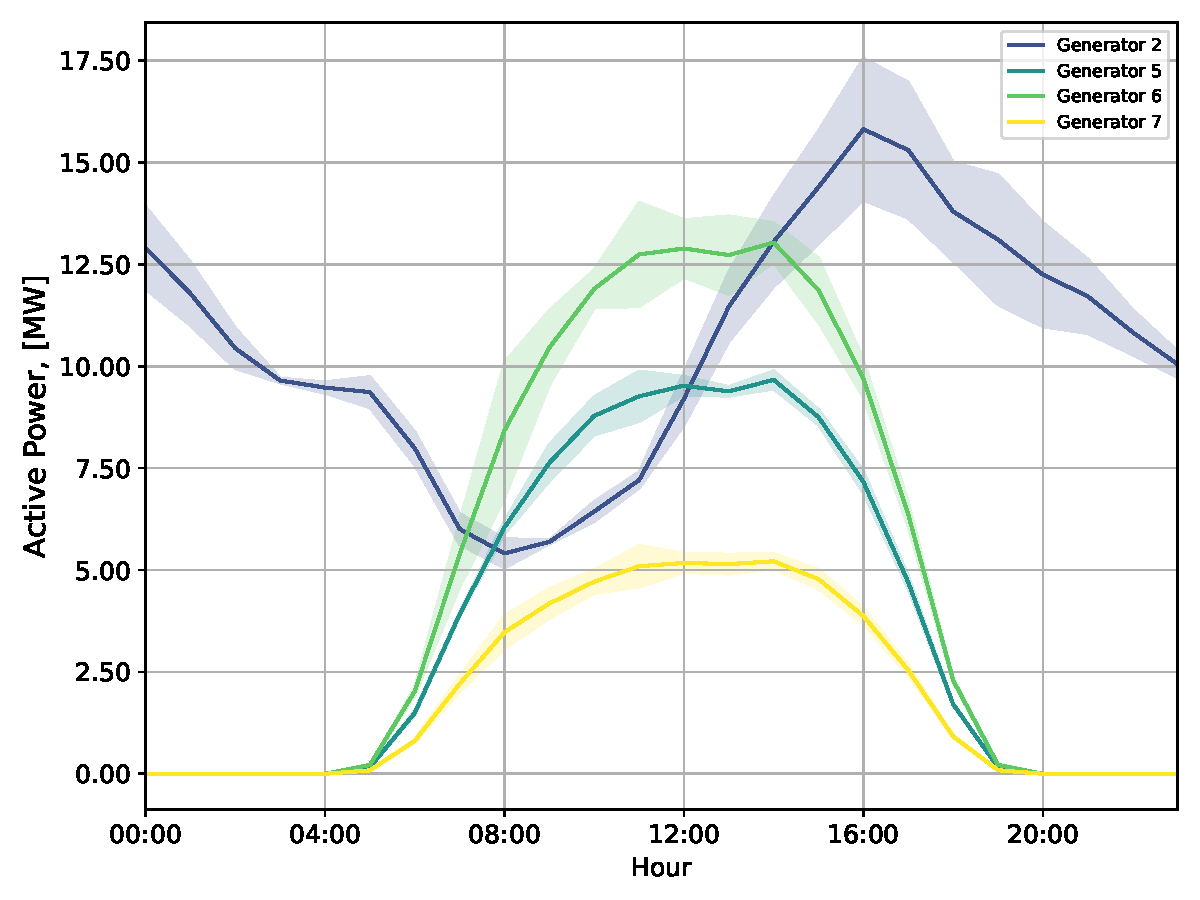
\includegraphics[width=0.475\textwidth]{case33_1_RES_generation_scenarios_2025_Spring.pdf}
    }
    \hfill
    \subfloat[Summer 2025]{
        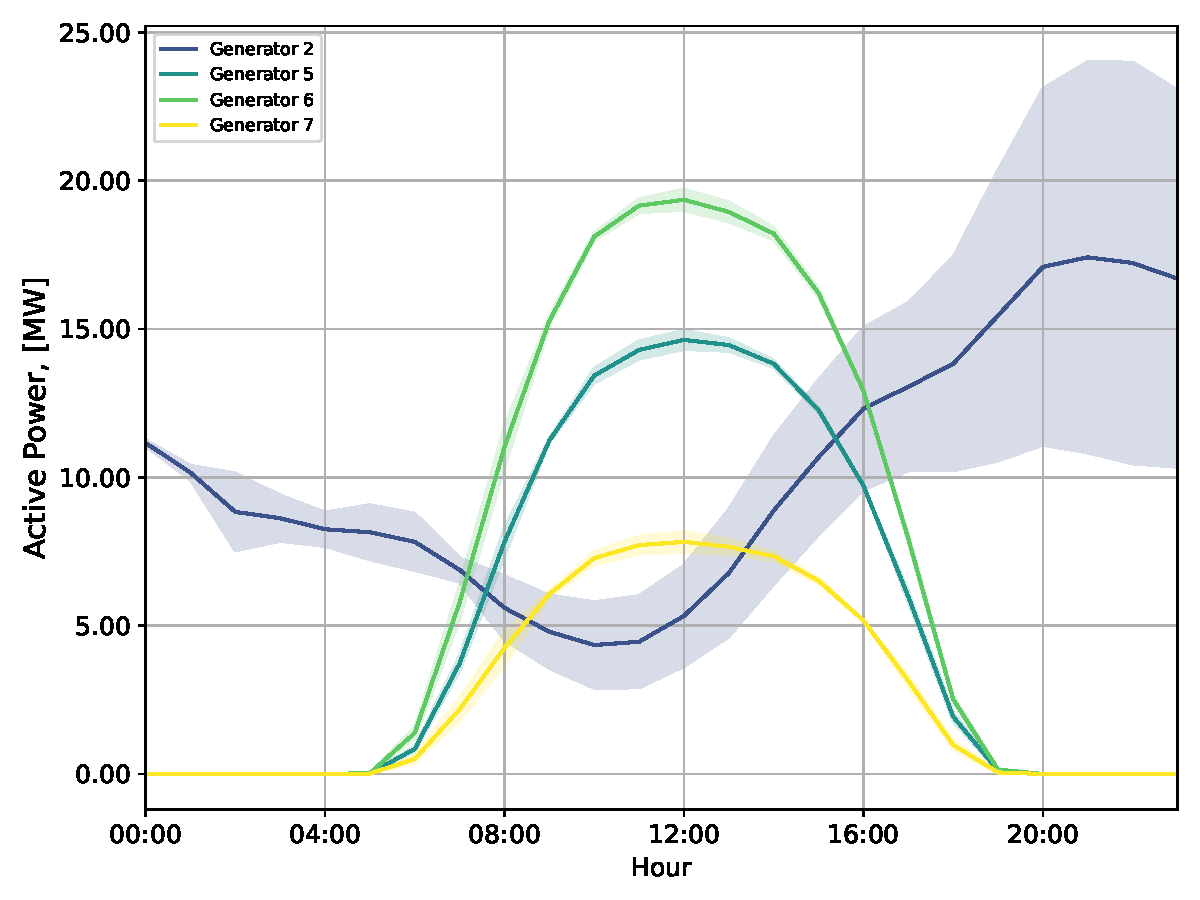
\includegraphics[width=0.475\textwidth]{case33_1_RES_generation_scenarios_2025_Summer.pdf}
    }
    \\[5pt]
    \subfloat[Autumn 2025]{
        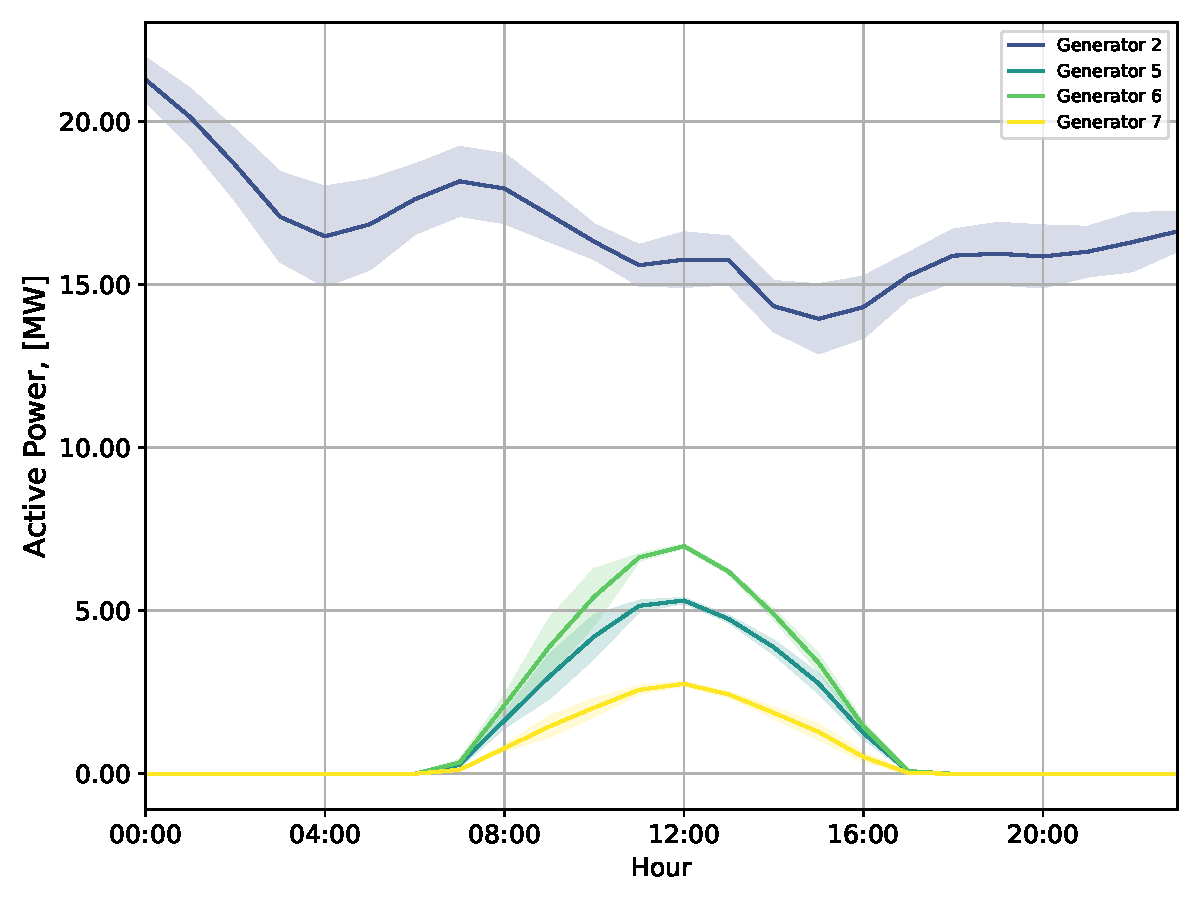
\includegraphics[width=0.475\textwidth]{case33_1_RES_generation_scenarios_2025_Autumn.pdf}
    }
    \hfill
    \subfloat[Winter 2025]{
        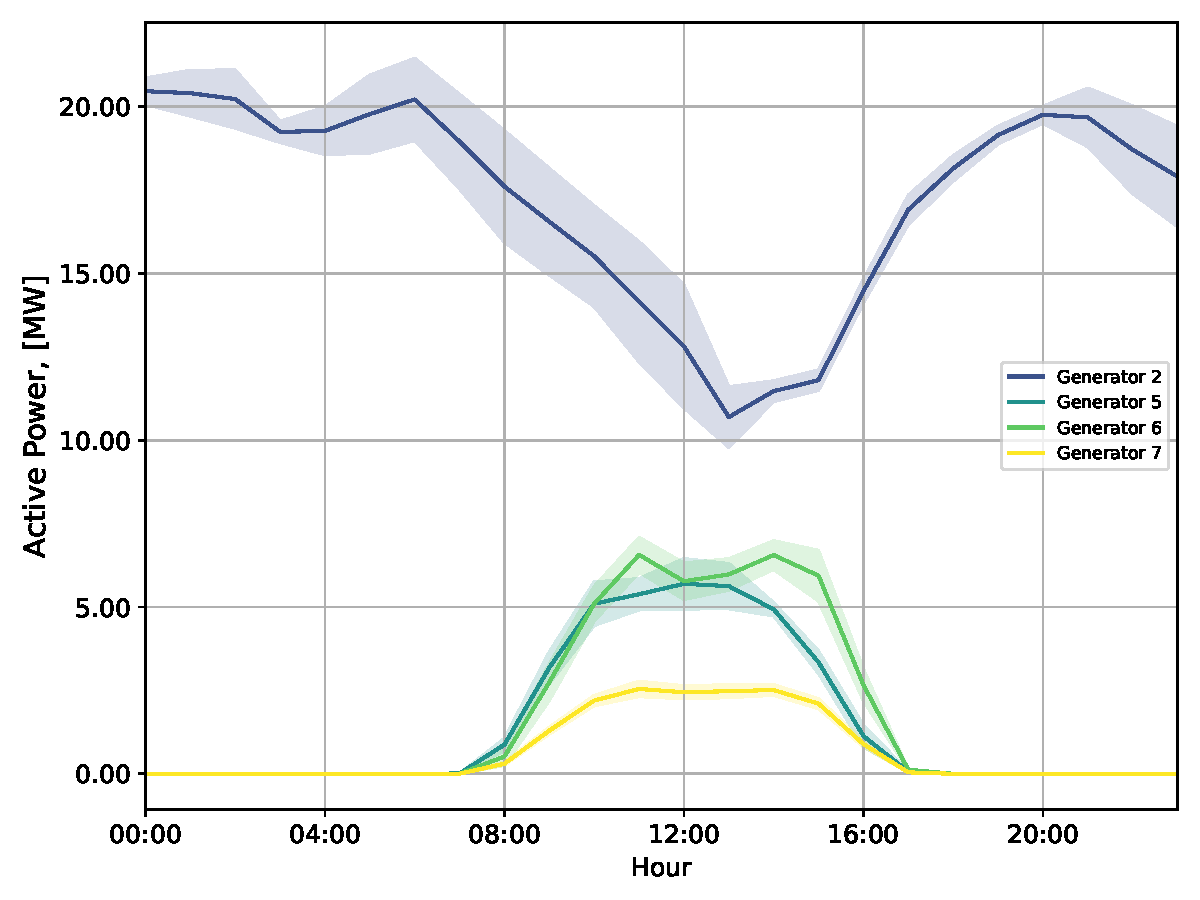
\includegraphics[width=0.475\textwidth]{case33_1_RES_generation_scenarios_2025_Winter.pdf}
    }
    \caption{ADN at TN node 5: RES profiles for 2025.}
    \label{fig:cs3_adn_node_5_res_scenarios_2025}
\end{figure*}

\begin{figure*}[htbp]
    \centering
    \subfloat[Spring 2025]{
        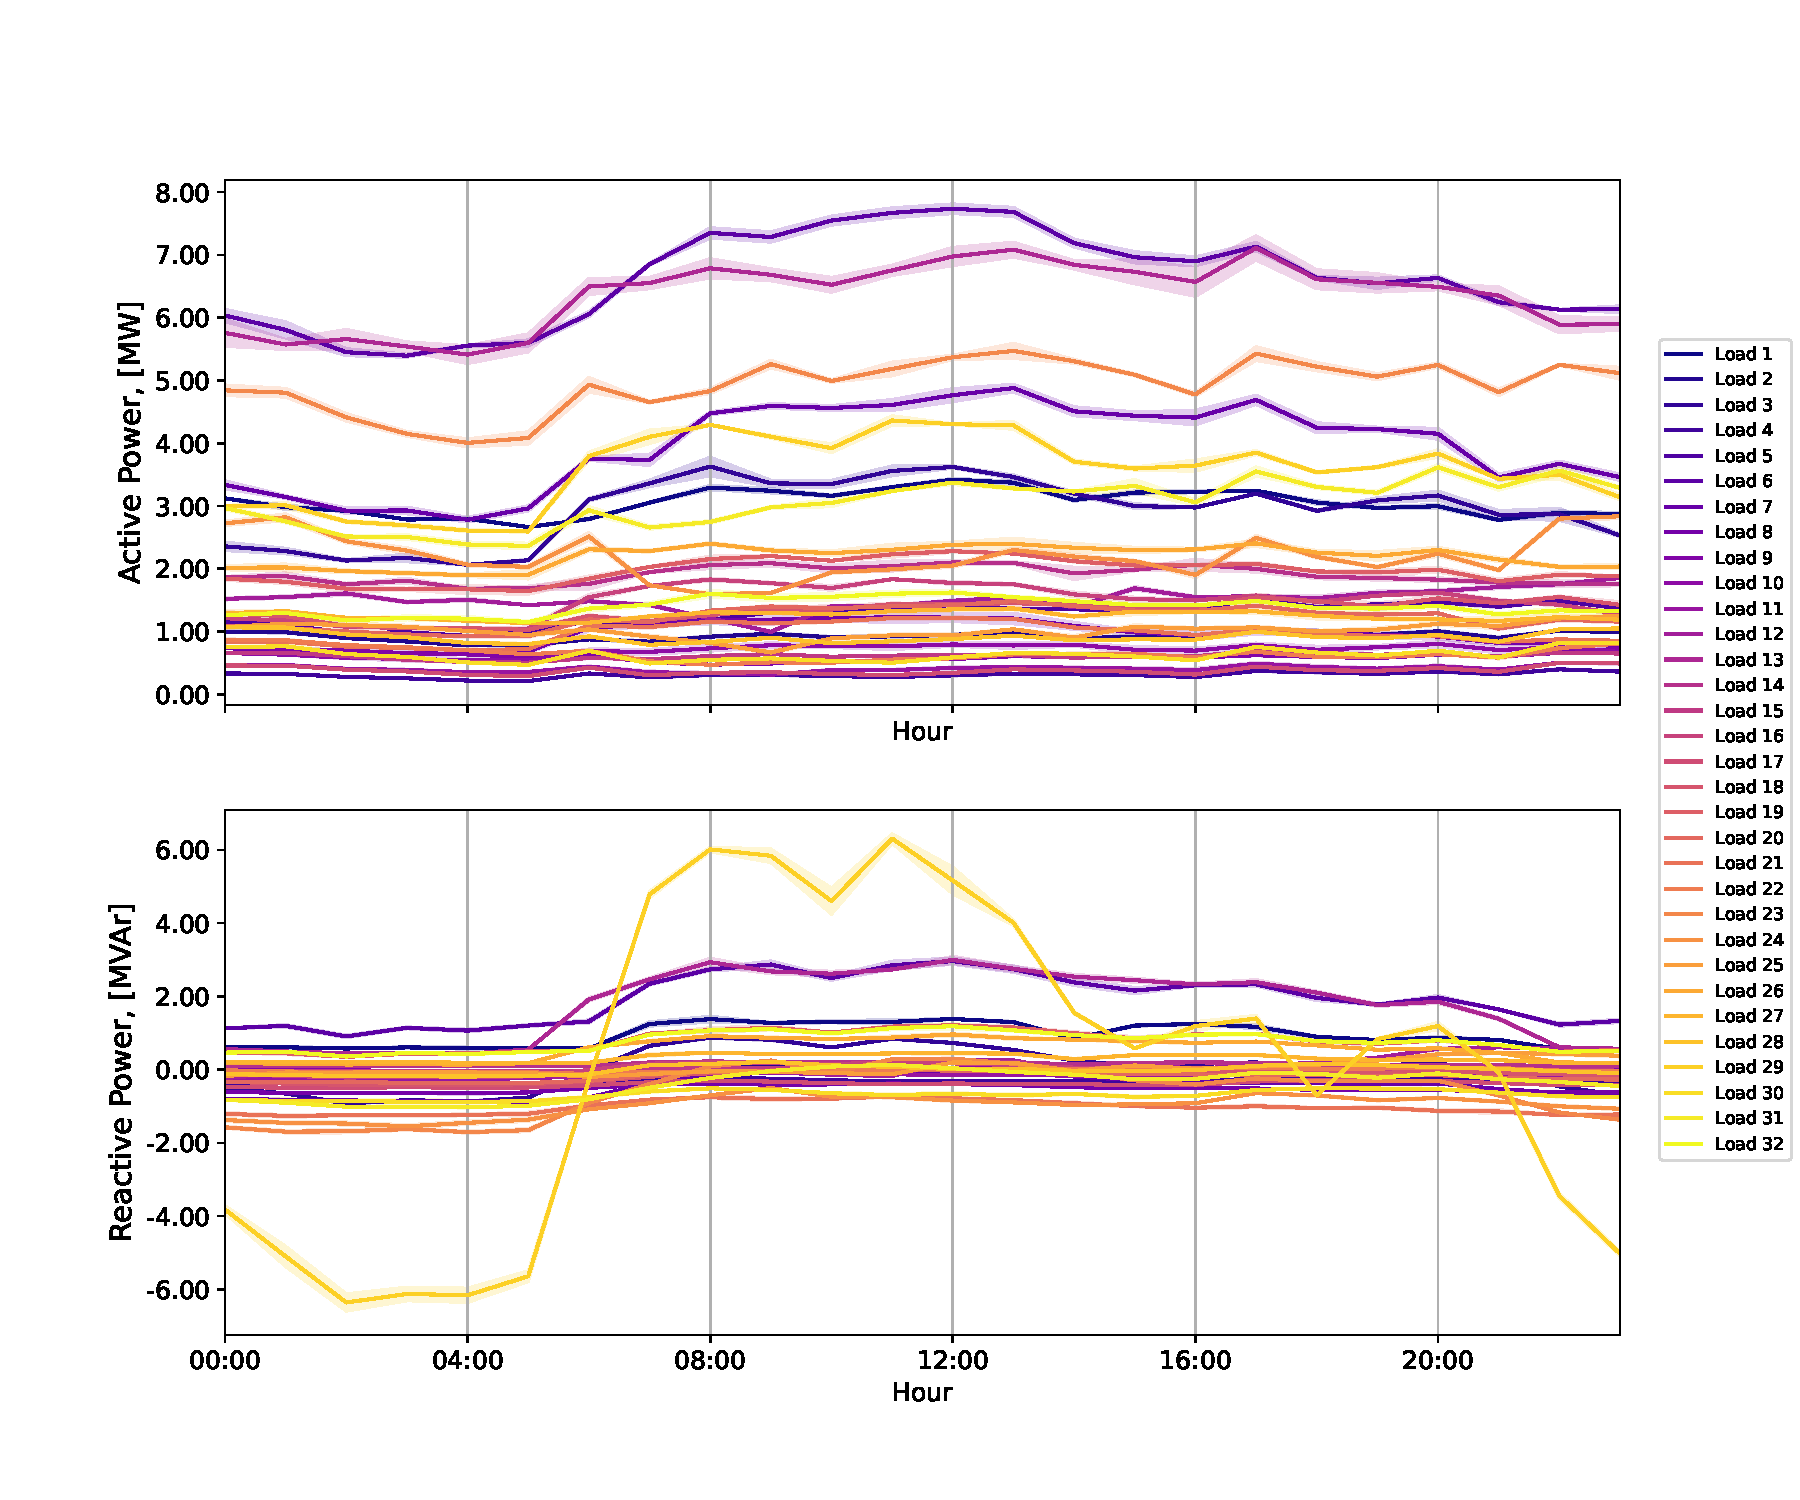
\includegraphics[width=0.475\textwidth]{case33_1_load_scenarios_2025_Spring.pdf}
    }
    \hfill
    \subfloat[Summer 2025]{
        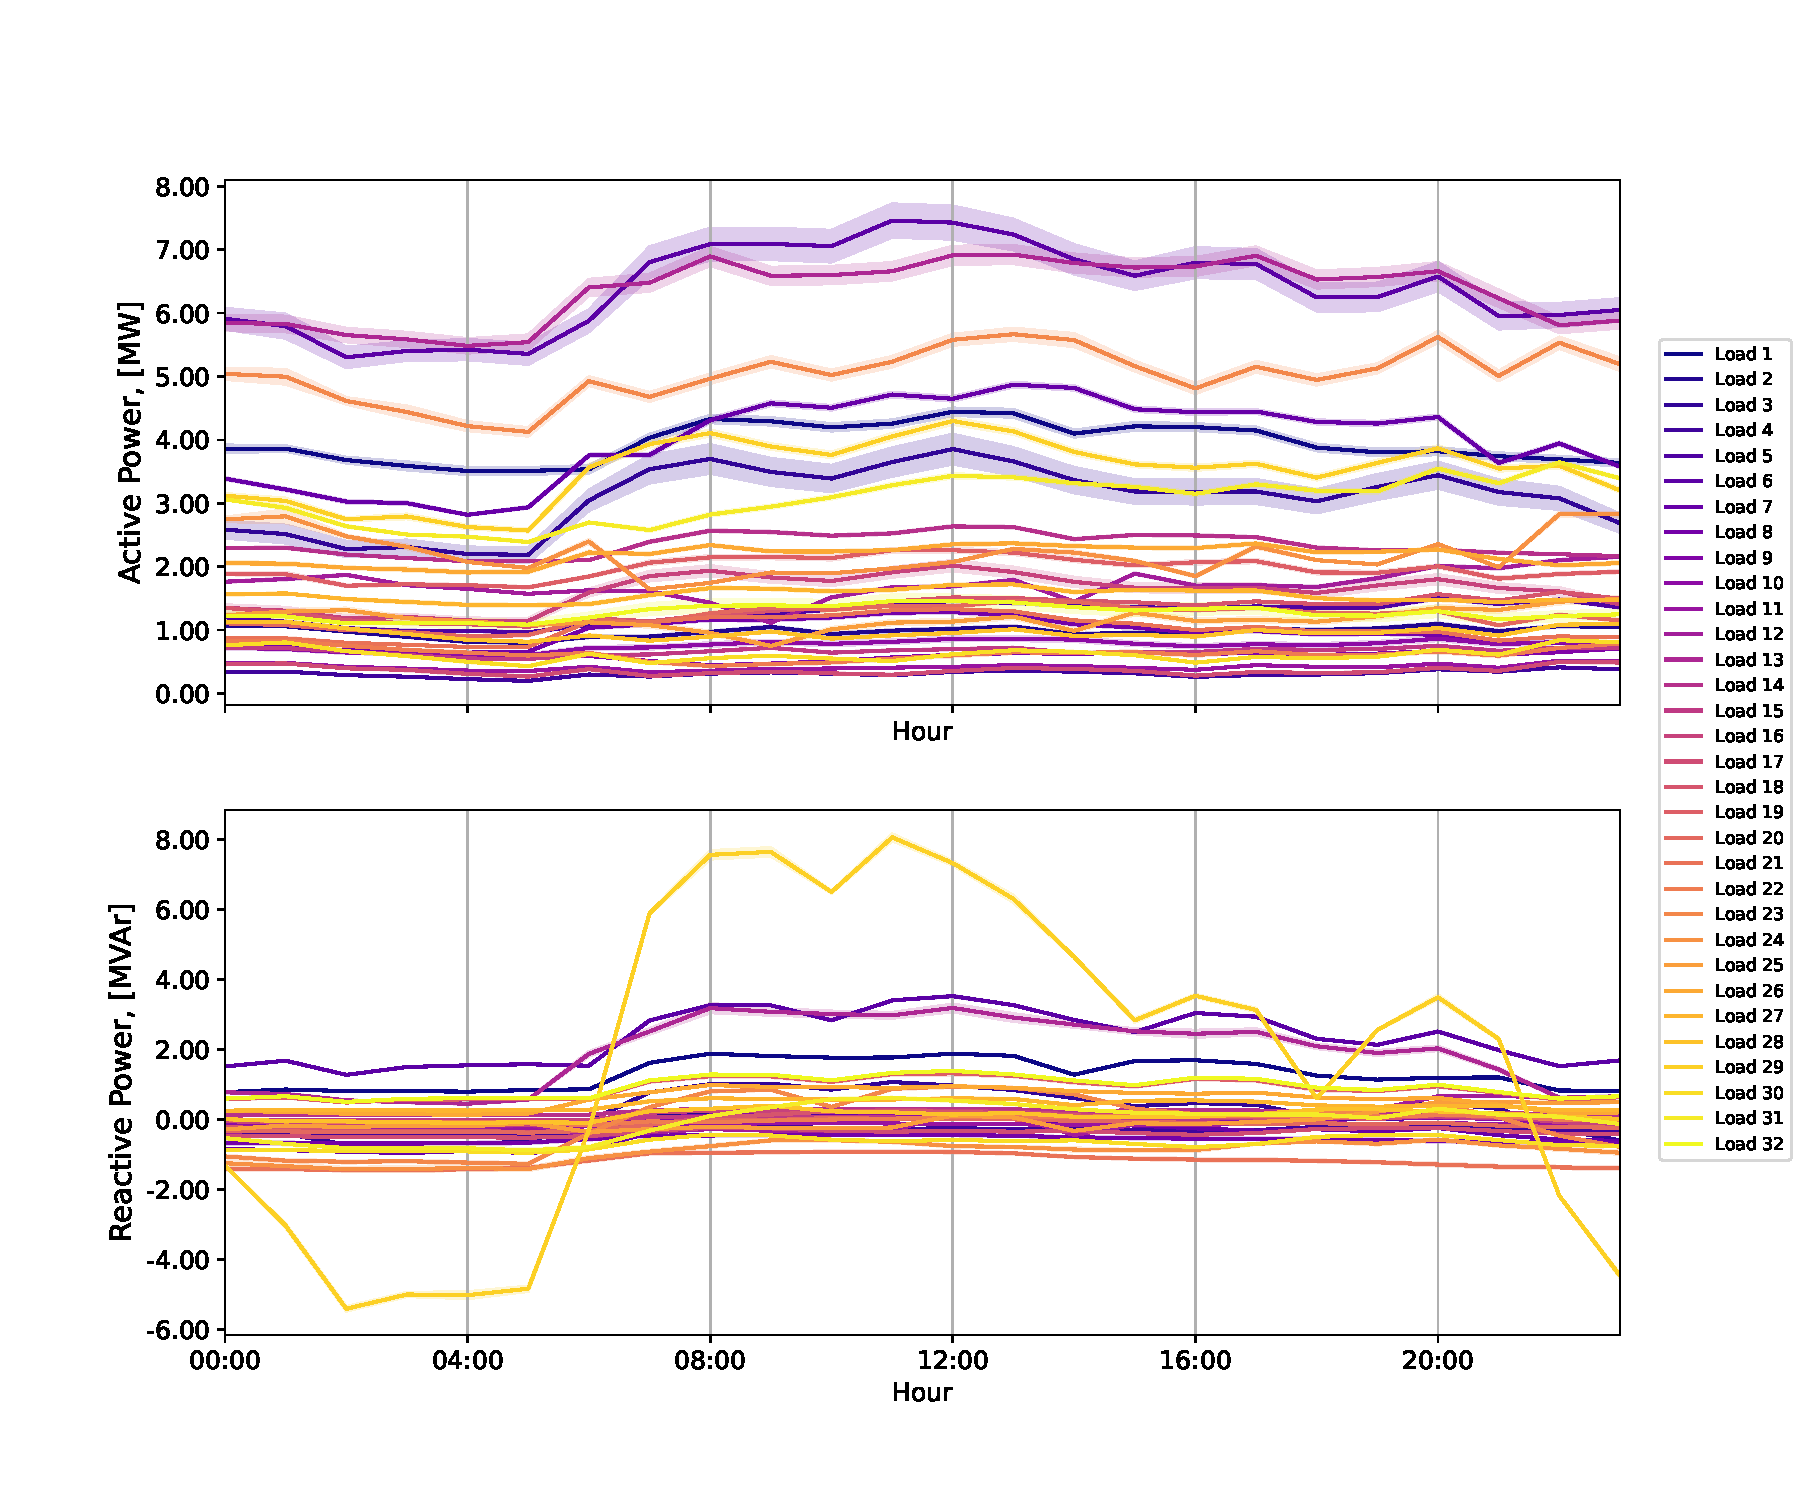
\includegraphics[width=0.475\textwidth]{case33_1_load_scenarios_2025_Summer.pdf}
    }
    \\[5pt]
    \subfloat[Autumn 2025]{
        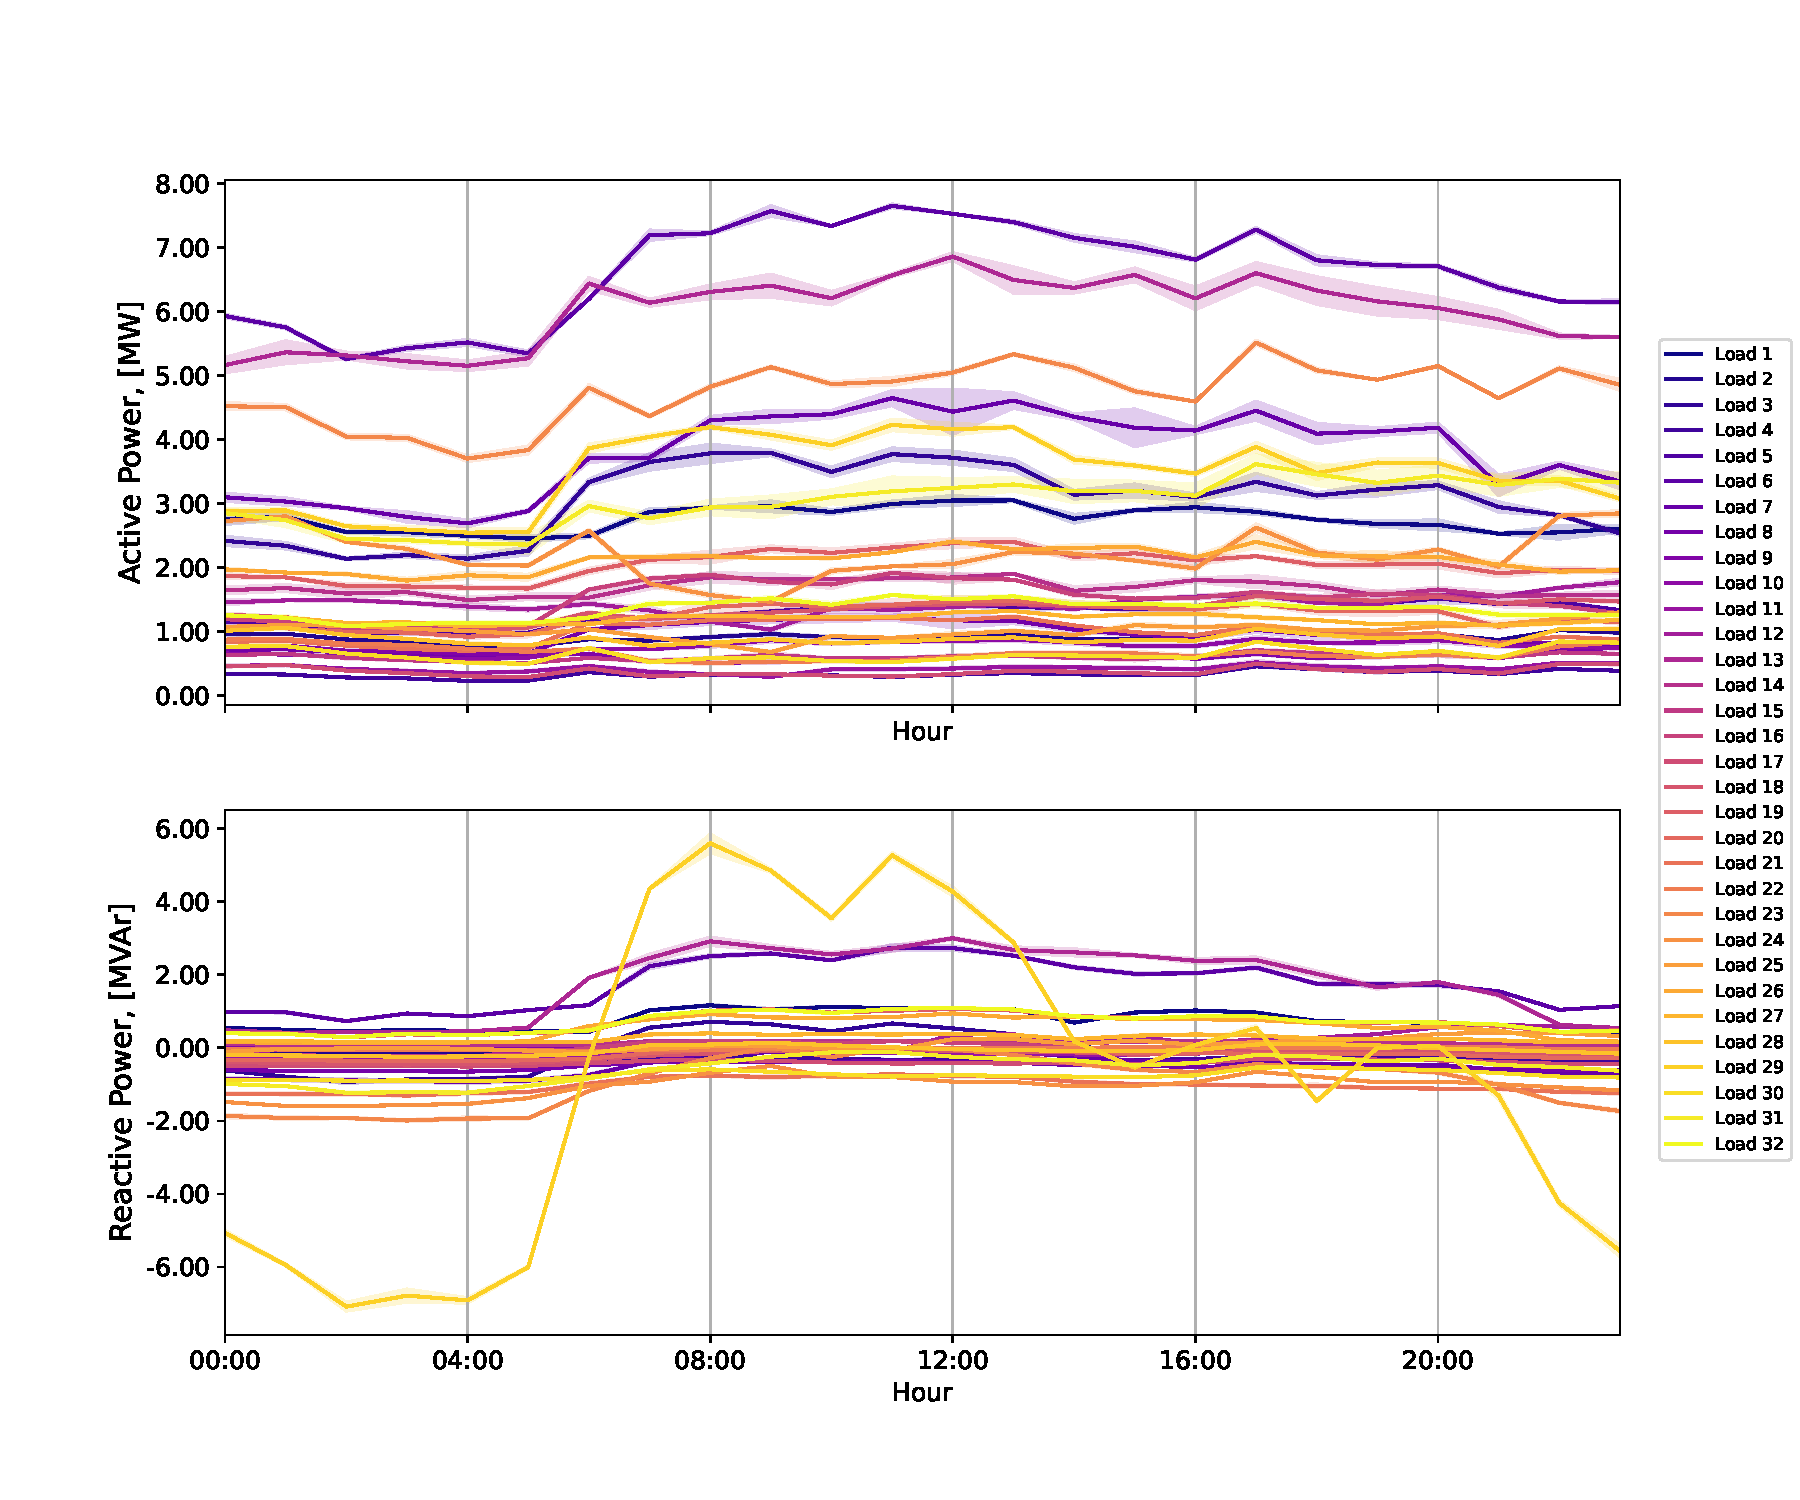
\includegraphics[width=0.475\textwidth]{case33_1_load_scenarios_2025_Autumn.pdf}
    }
    \hfill
    \subfloat[Winter 2025]{
        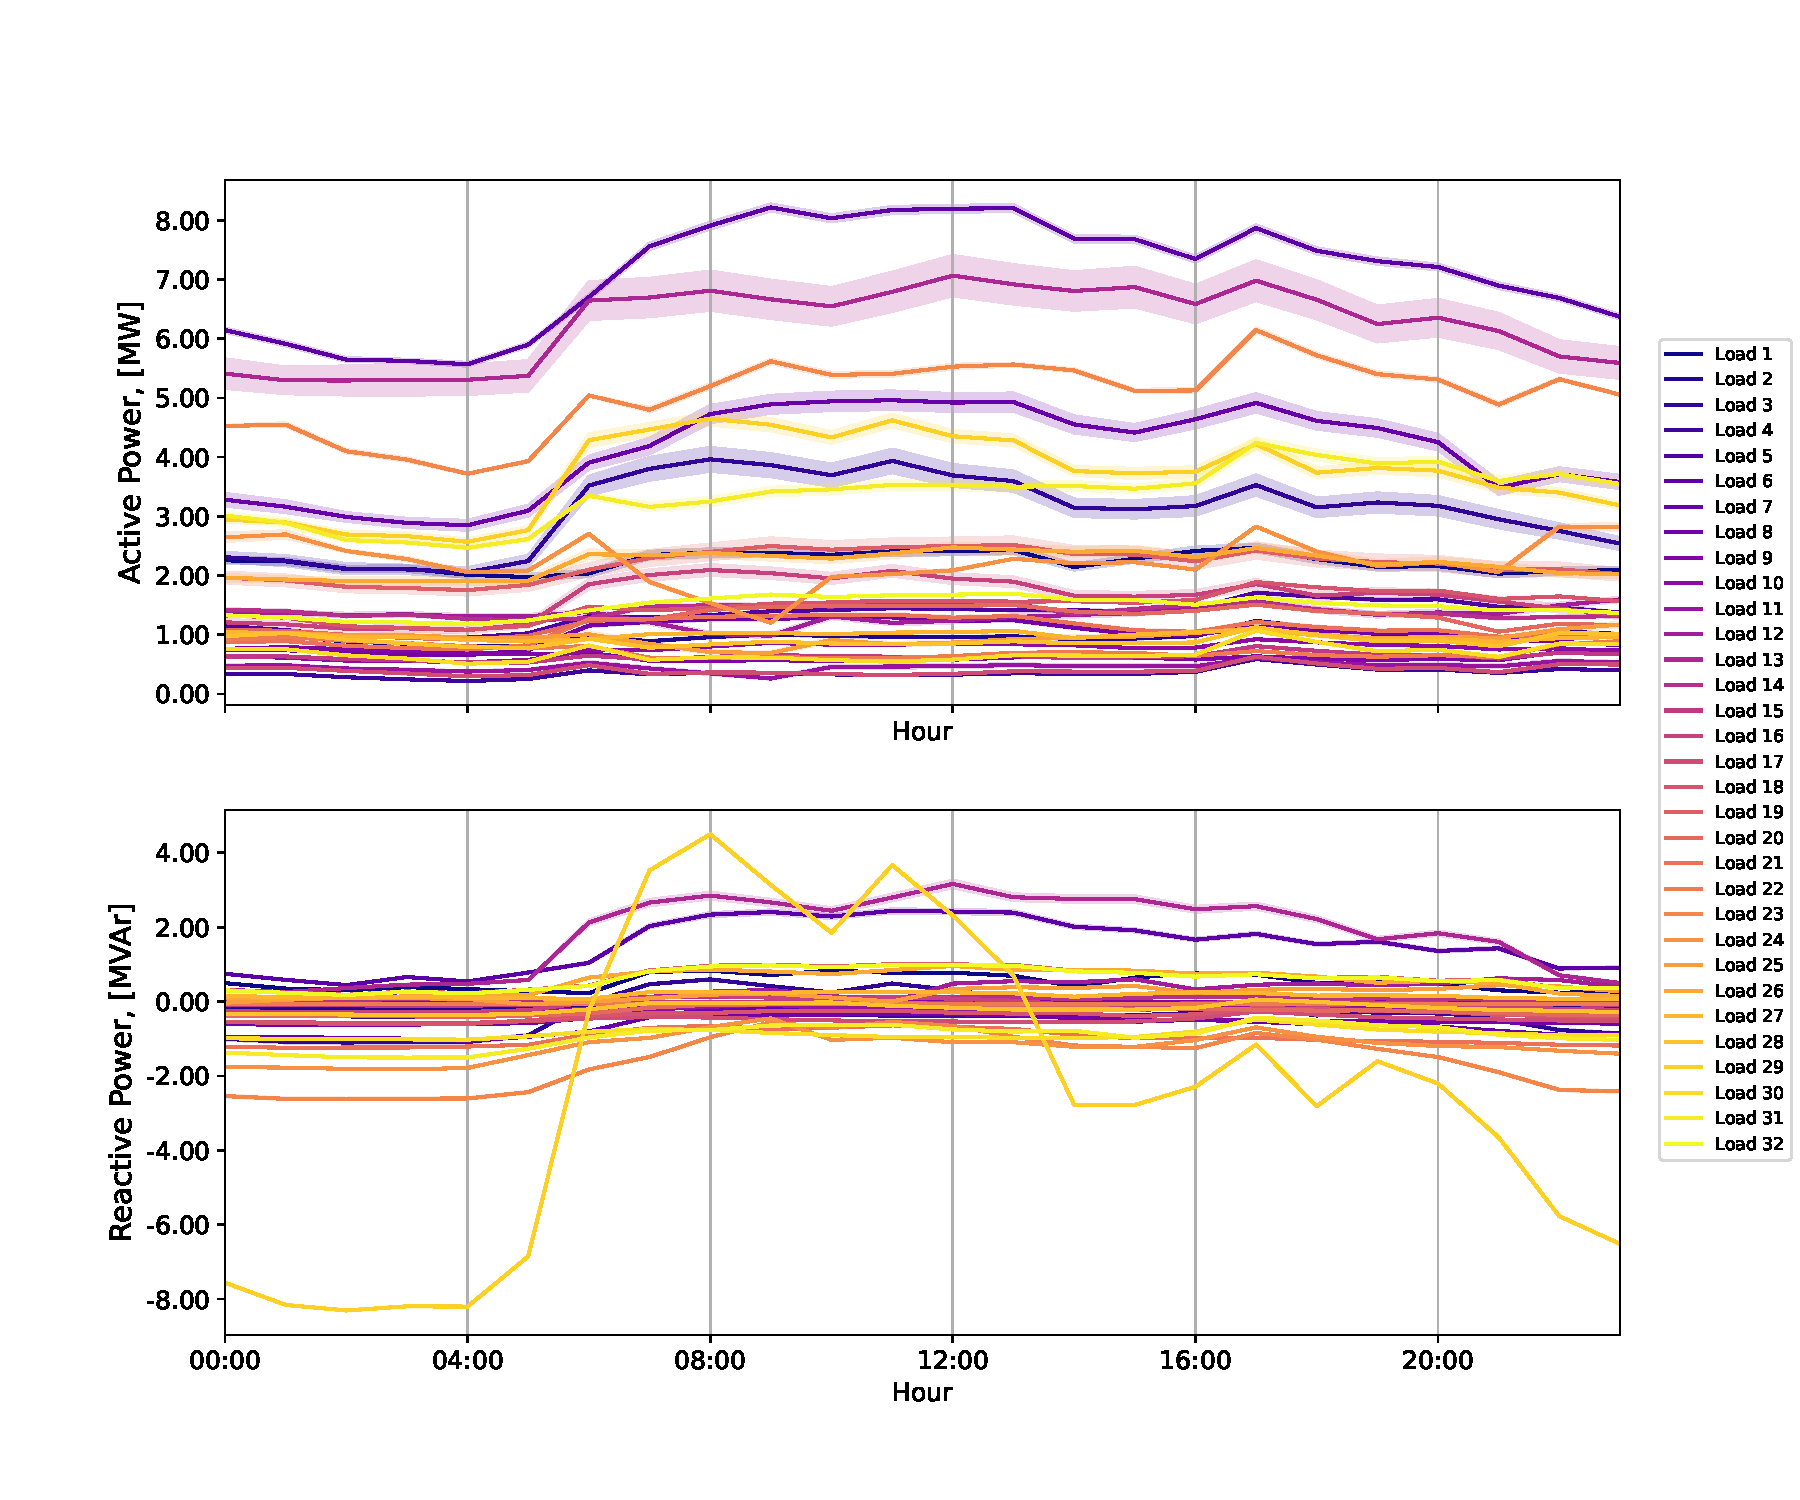
\includegraphics[width=0.475\textwidth]{case33_1_load_scenarios_2025_Winter.pdf}
    }
    \caption{ADN at TN node 5: load profiles for 2025.}
    \label{fig:cs3_adn_node_5_load_scenarios_2025}
\end{figure*}

\begin{figure}[htbp!]
    \centering
    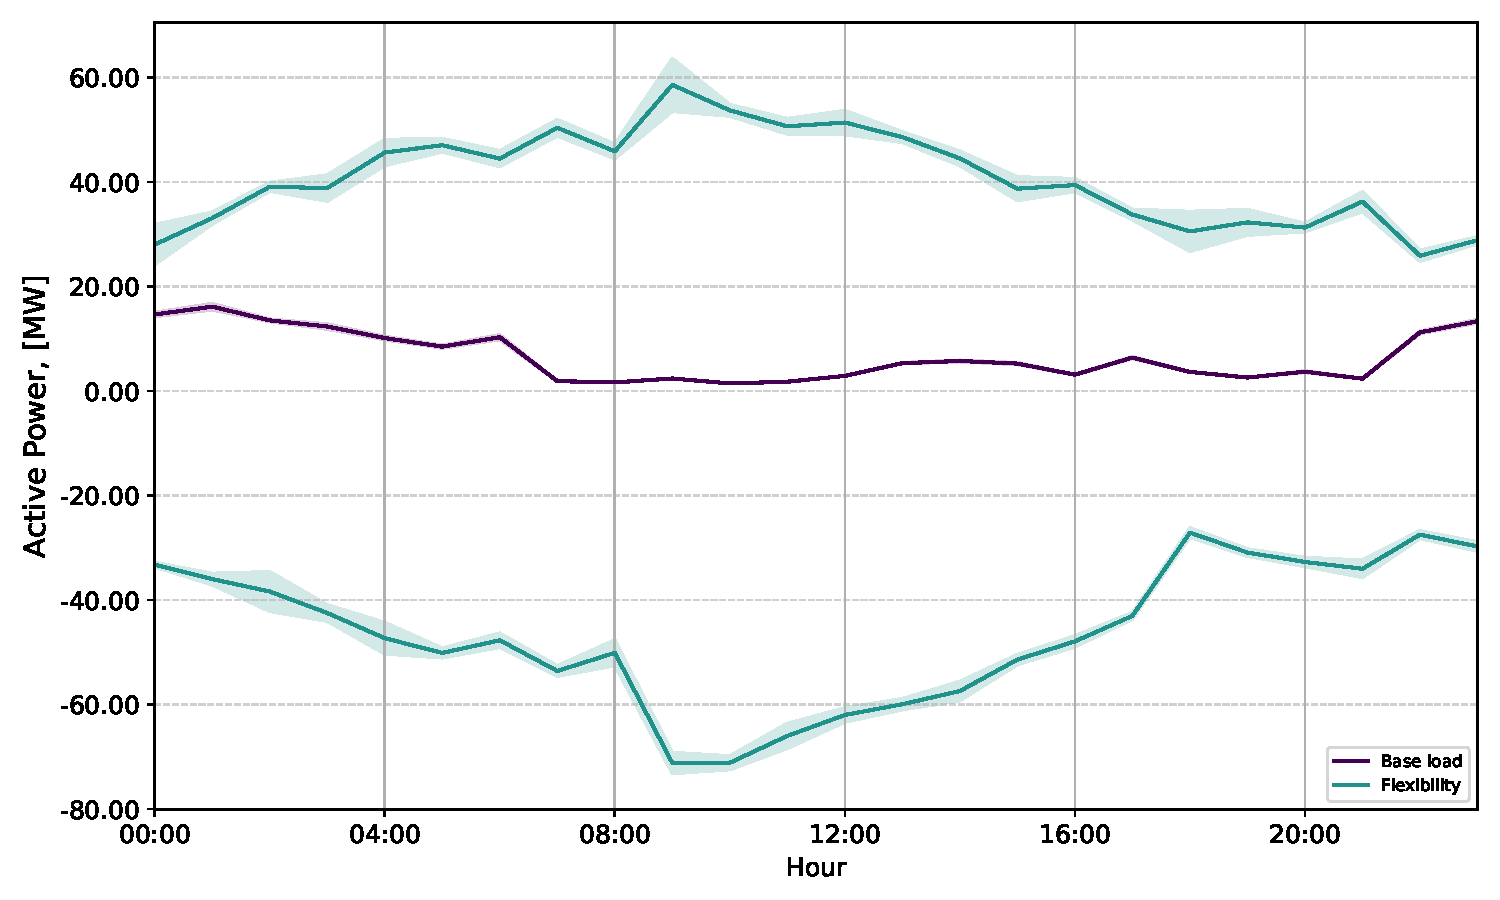
\includegraphics[width=0.65\textwidth]{case33_1_flexibility_scenarios_2025_Spring.pdf}
    \caption{Flexible load profiles for the ADN at TN node~5.}
    \label{fig:cs3_adn_node_5_flexibility}
\end{figure}

\subsection{ADN Connected to TN Node~7}
\label{app:adn_node7_description}

Figure~\ref{fig:cs3_adn_node_7_res_scenarios_2025} and Figure~\ref{fig:cs3_adn_node_7_load_scenarios_2025} show the RES generation and load profiles for the spring, summer, autumn, and winter representative days of 2025 for the ADN at TN node~7. Figure~\ref{fig:cs3_adn_node_7_flexibility} shows the flexible load profiles adopted for this ADN.

\begin{figure*}[htbp]
    \centering
    \subfloat[Spring 2025]{
        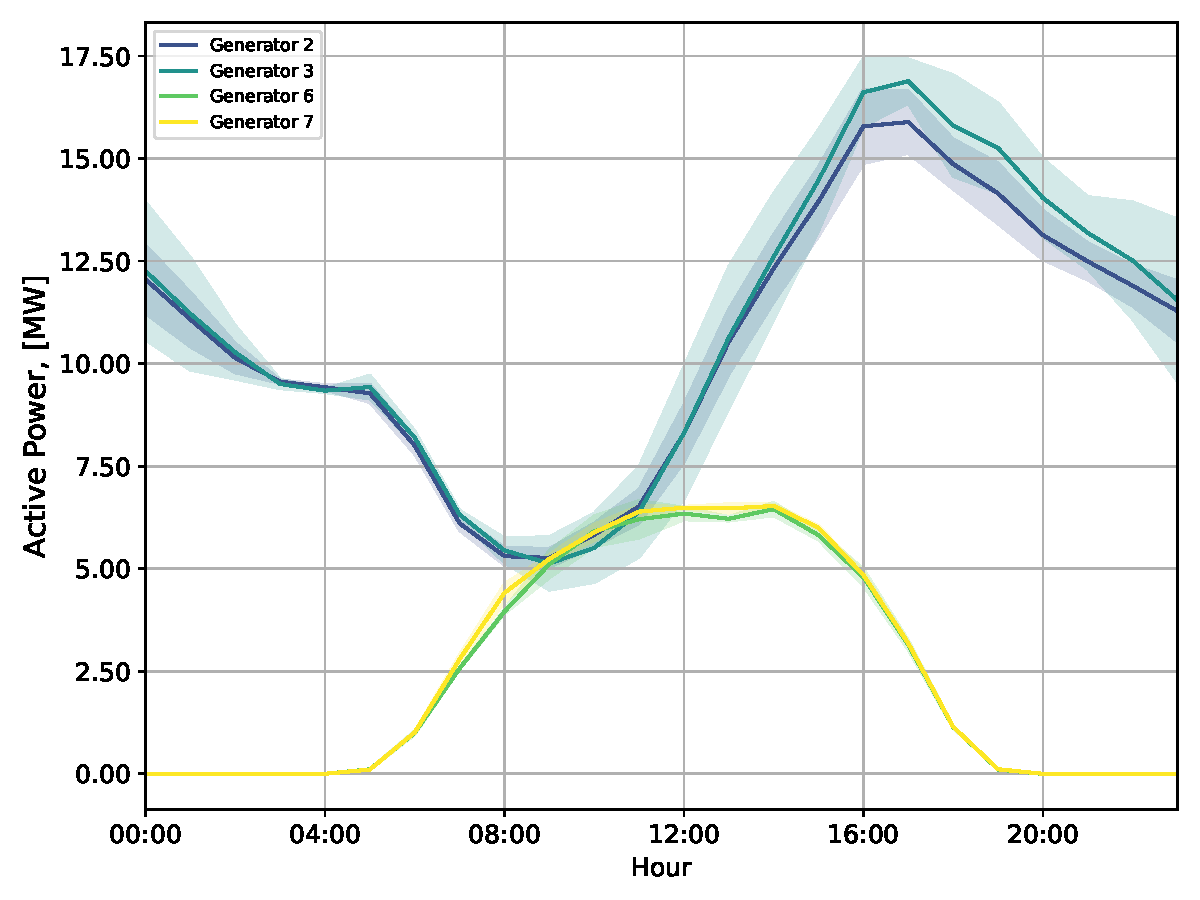
\includegraphics[width=0.475\textwidth]{case33_2_RES_generation_scenarios_2025_Spring.pdf}
    }
    \hfill
    \subfloat[Summer 2025]{
        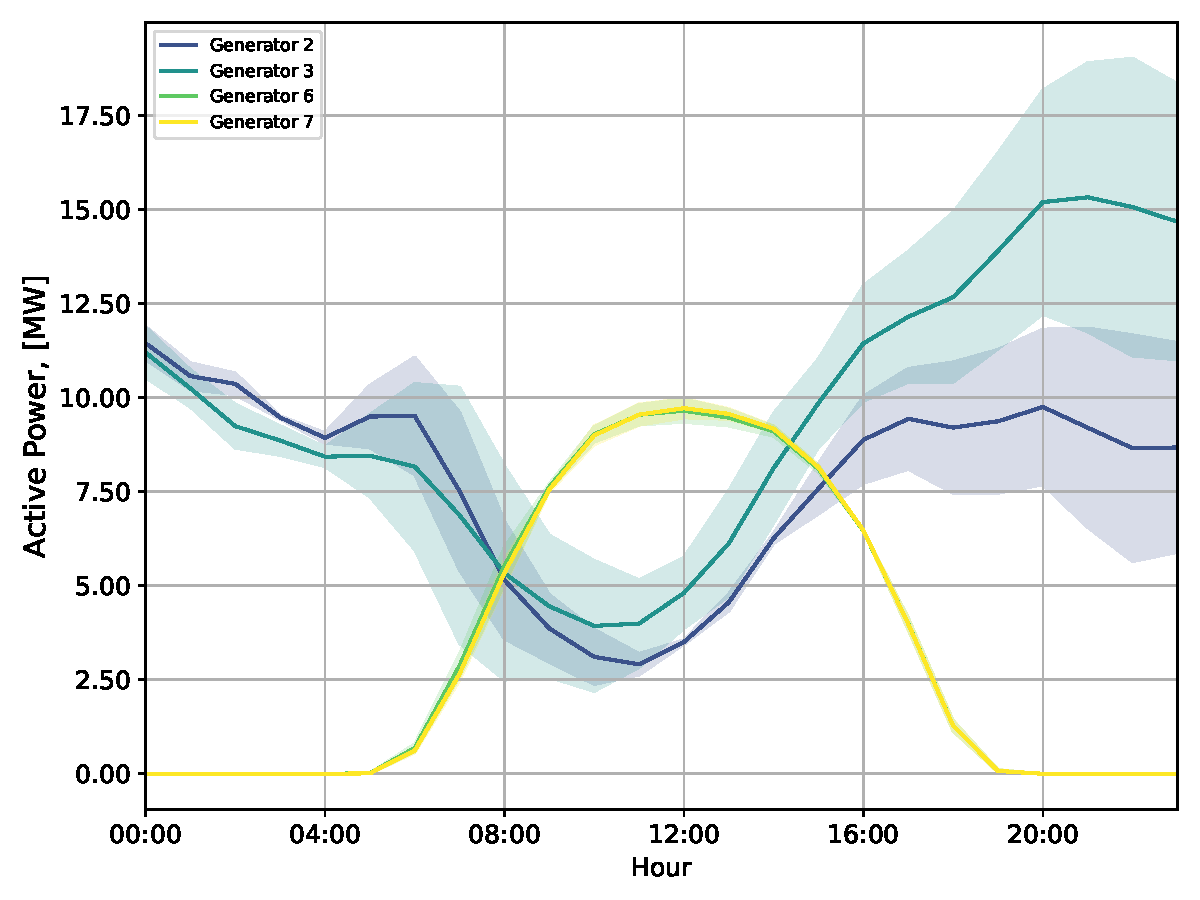
\includegraphics[width=0.475\textwidth]{case33_2_RES_generation_scenarios_2025_Summer.pdf}
    }
    \\[5pt]
    \subfloat[Autumn 2025]{
        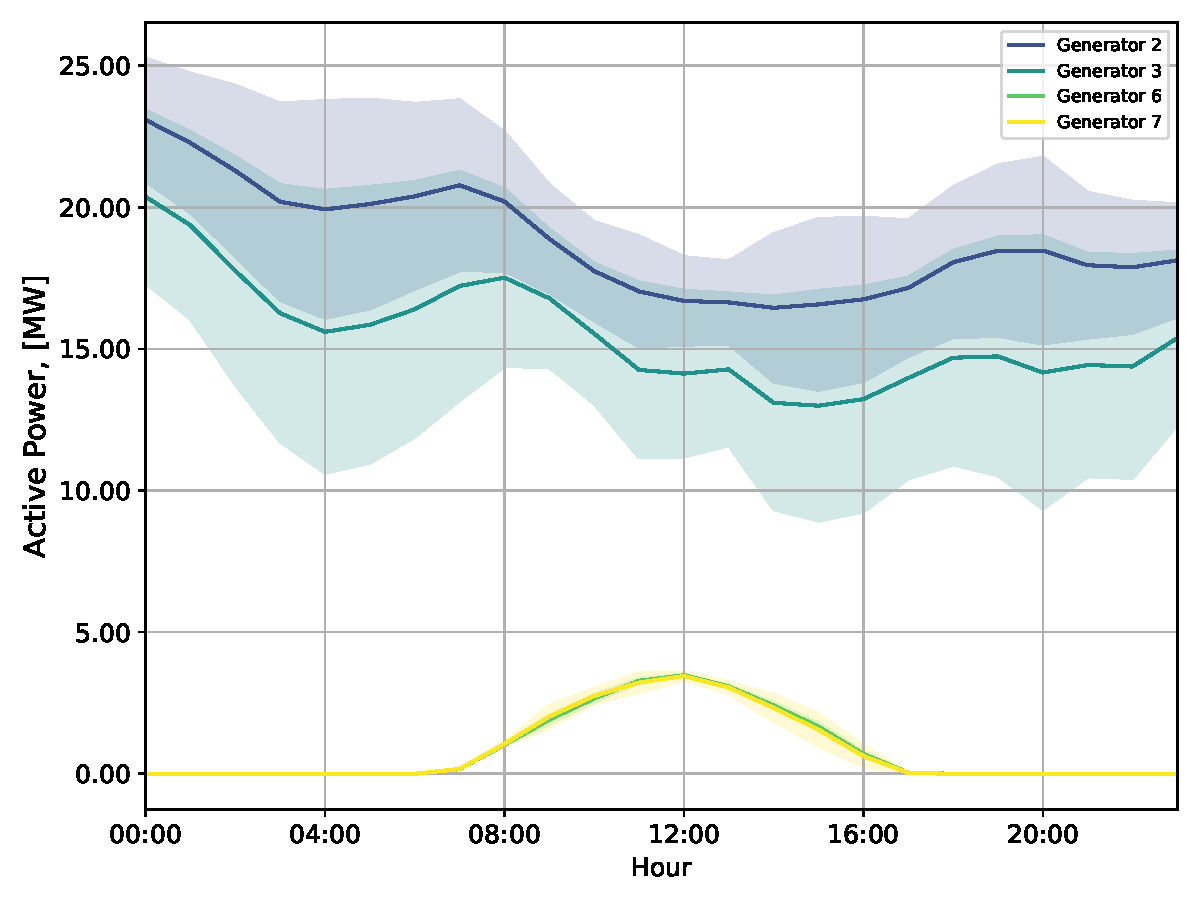
\includegraphics[width=0.475\textwidth]{case33_2_RES_generation_scenarios_2025_Autumn.pdf}
    }
    \hfill
    \subfloat[Winter 2025]{
        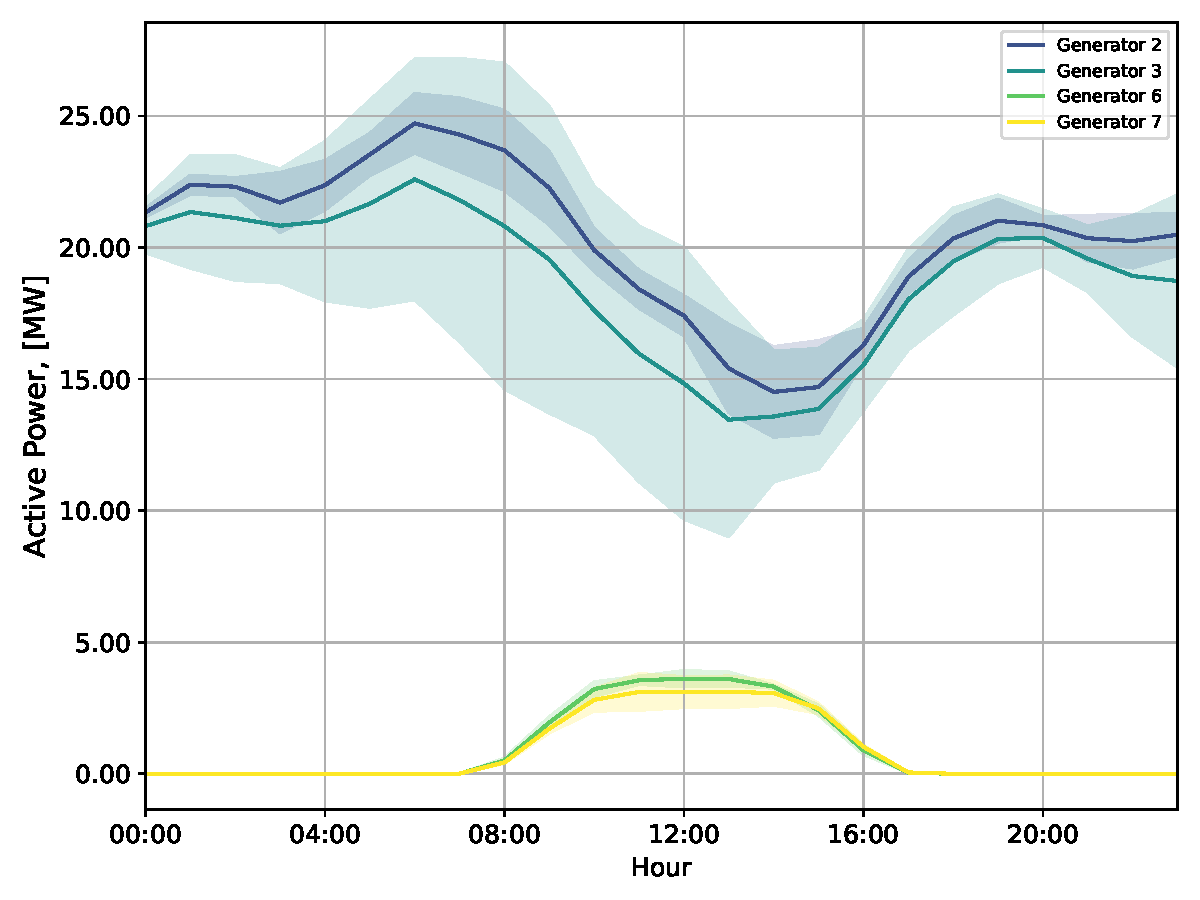
\includegraphics[width=0.475\textwidth]{case33_2_RES_generation_scenarios_2025_Winter.pdf}
    }
    \caption{ADN at TN node 7: RES profiles for 2025.}
    \label{fig:cs3_adn_node_7_res_scenarios_2025}
\end{figure*}

\begin{figure*}[htbp]
    \centering
    \subfloat[Spring 2025]{
        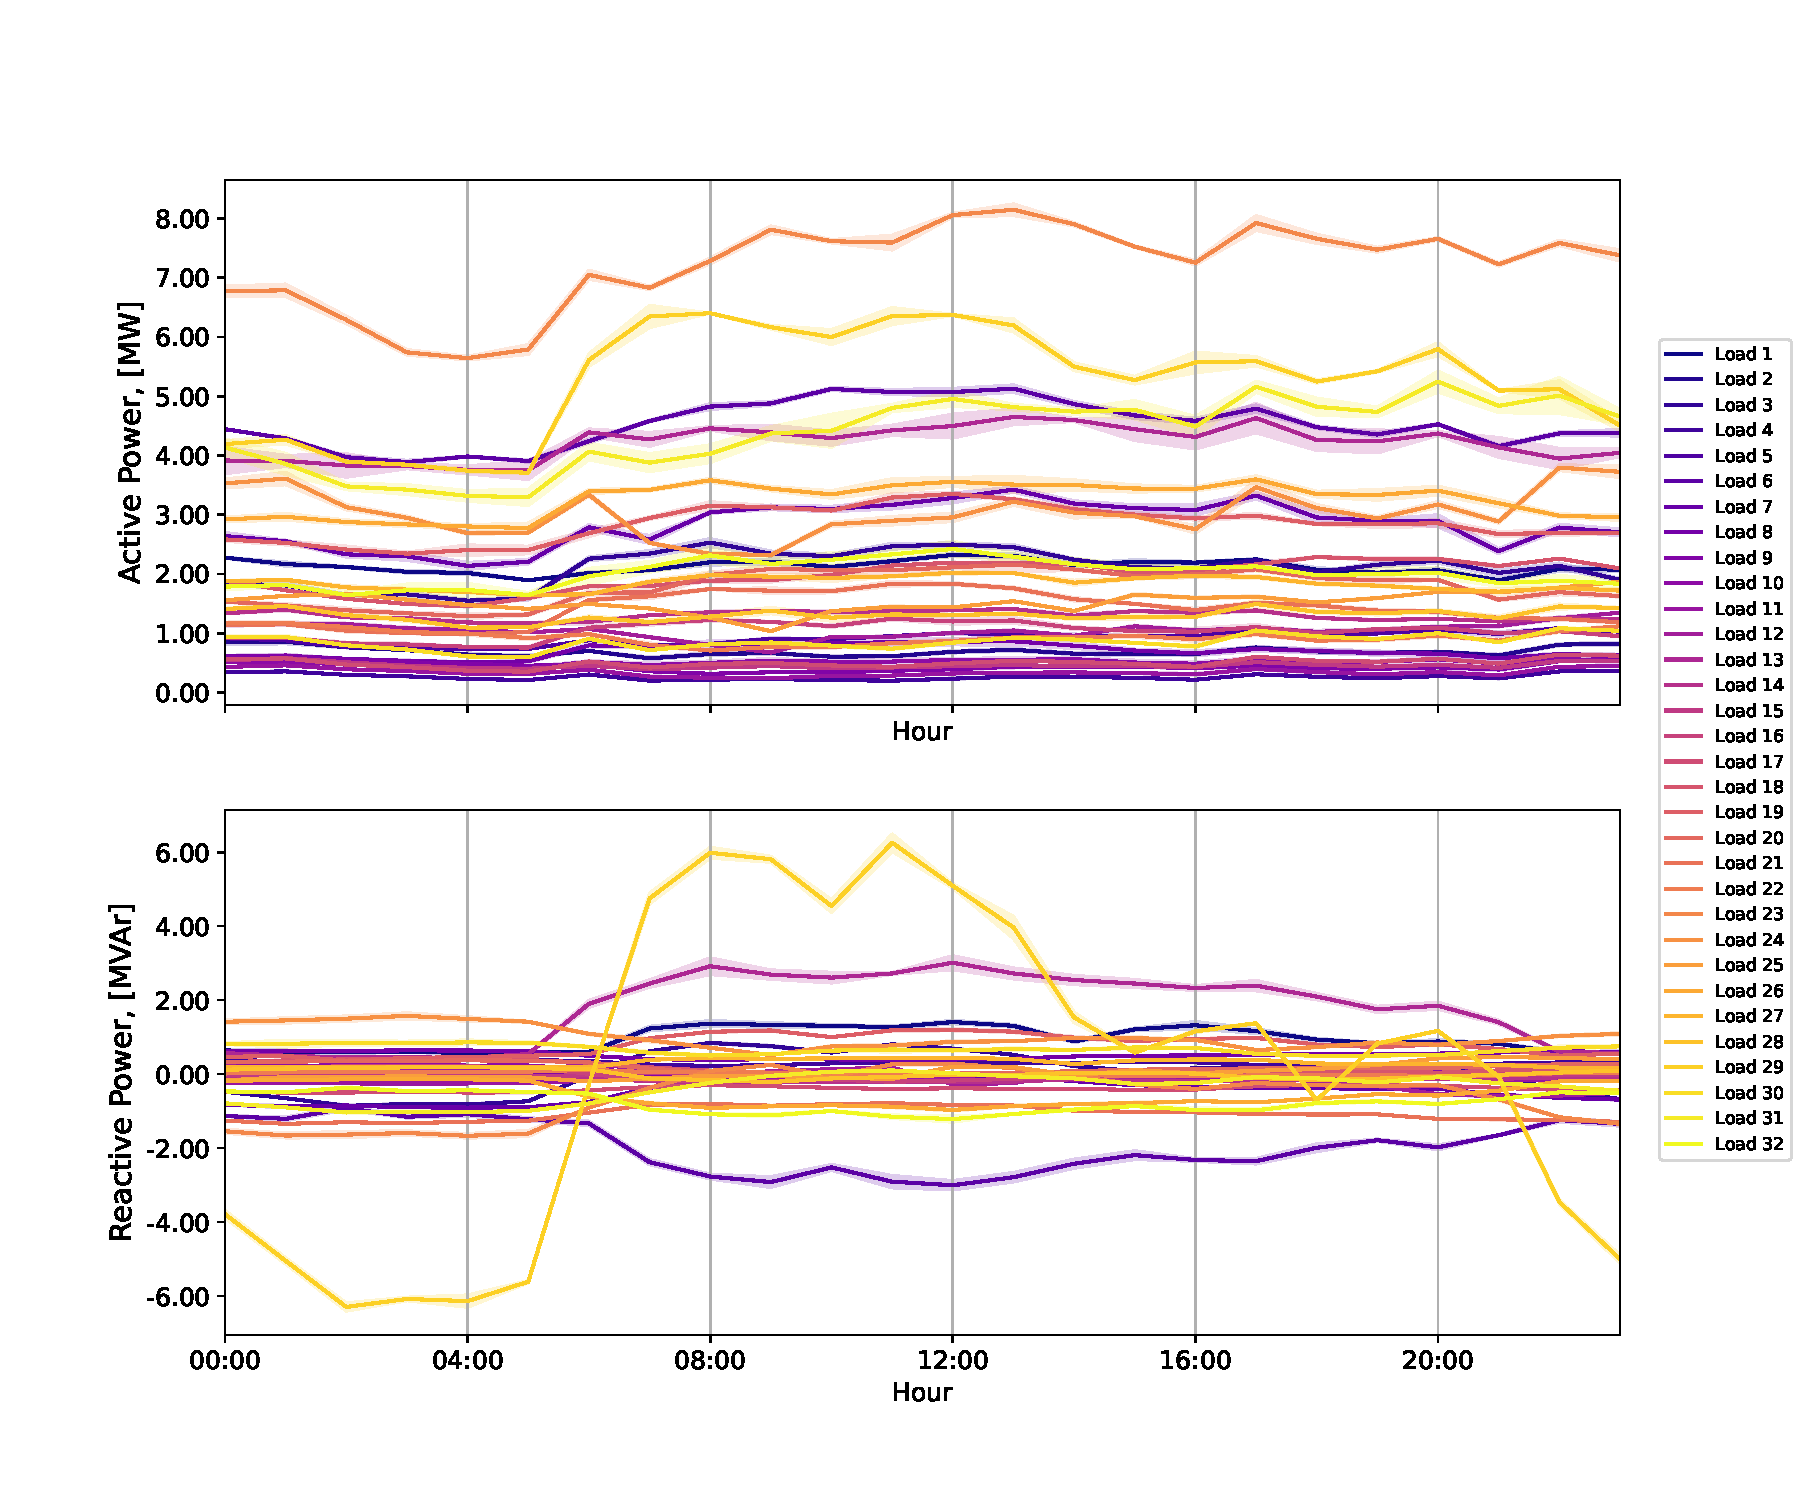
\includegraphics[width=0.475\textwidth]{case33_2_load_scenarios_2025_Spring.pdf}
    }
    \hfill
    \subfloat[Summer 2025]{
        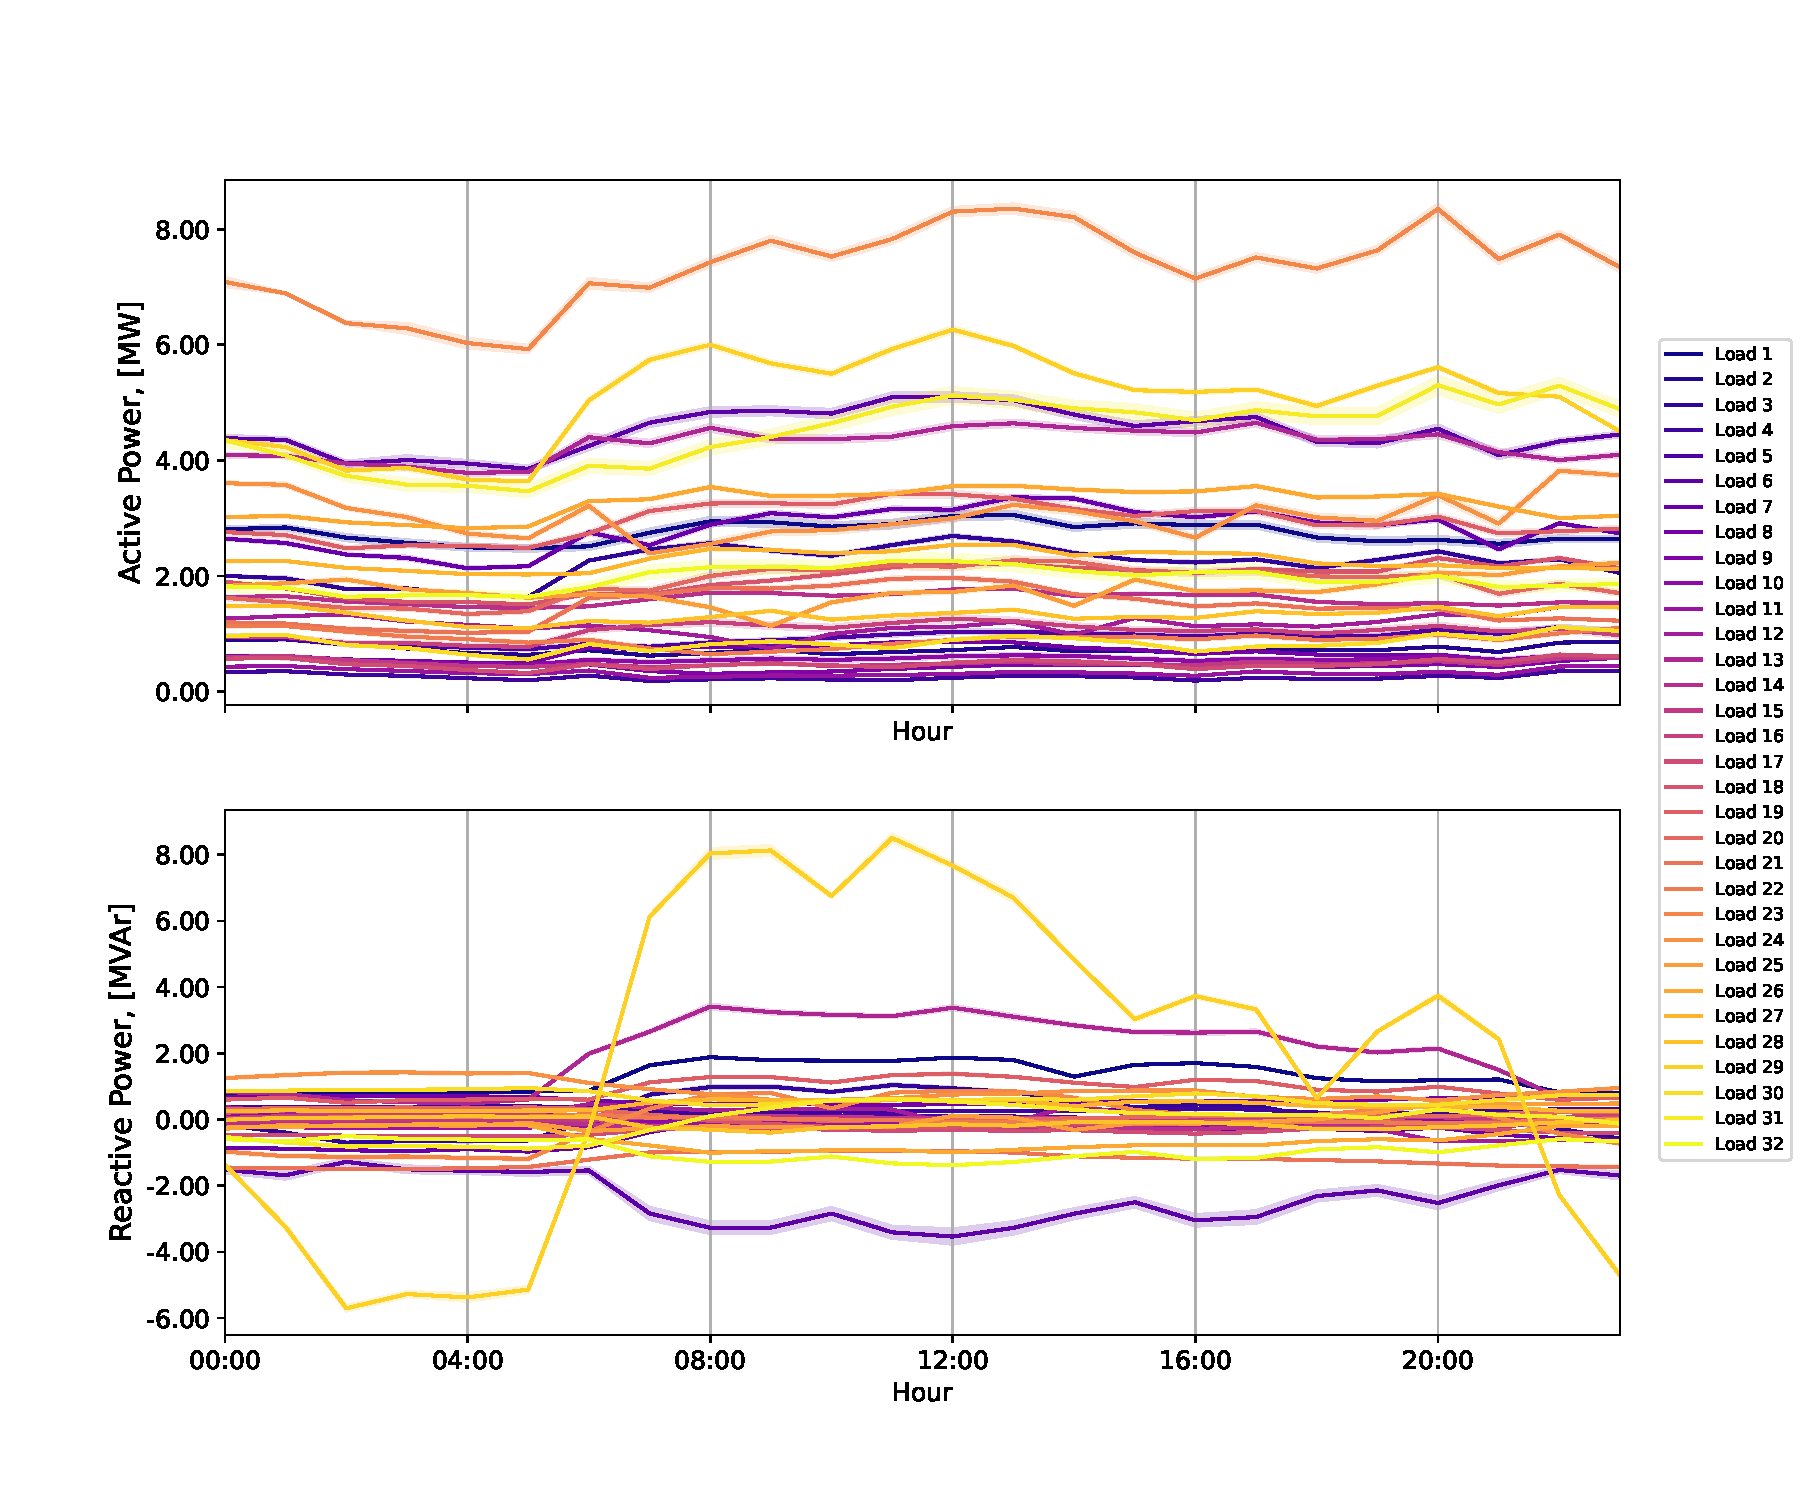
\includegraphics[width=0.475\textwidth]{case33_2_load_scenarios_2025_Summer.pdf}
    }
    \\[5pt]
    \subfloat[Autumn 2025]{
        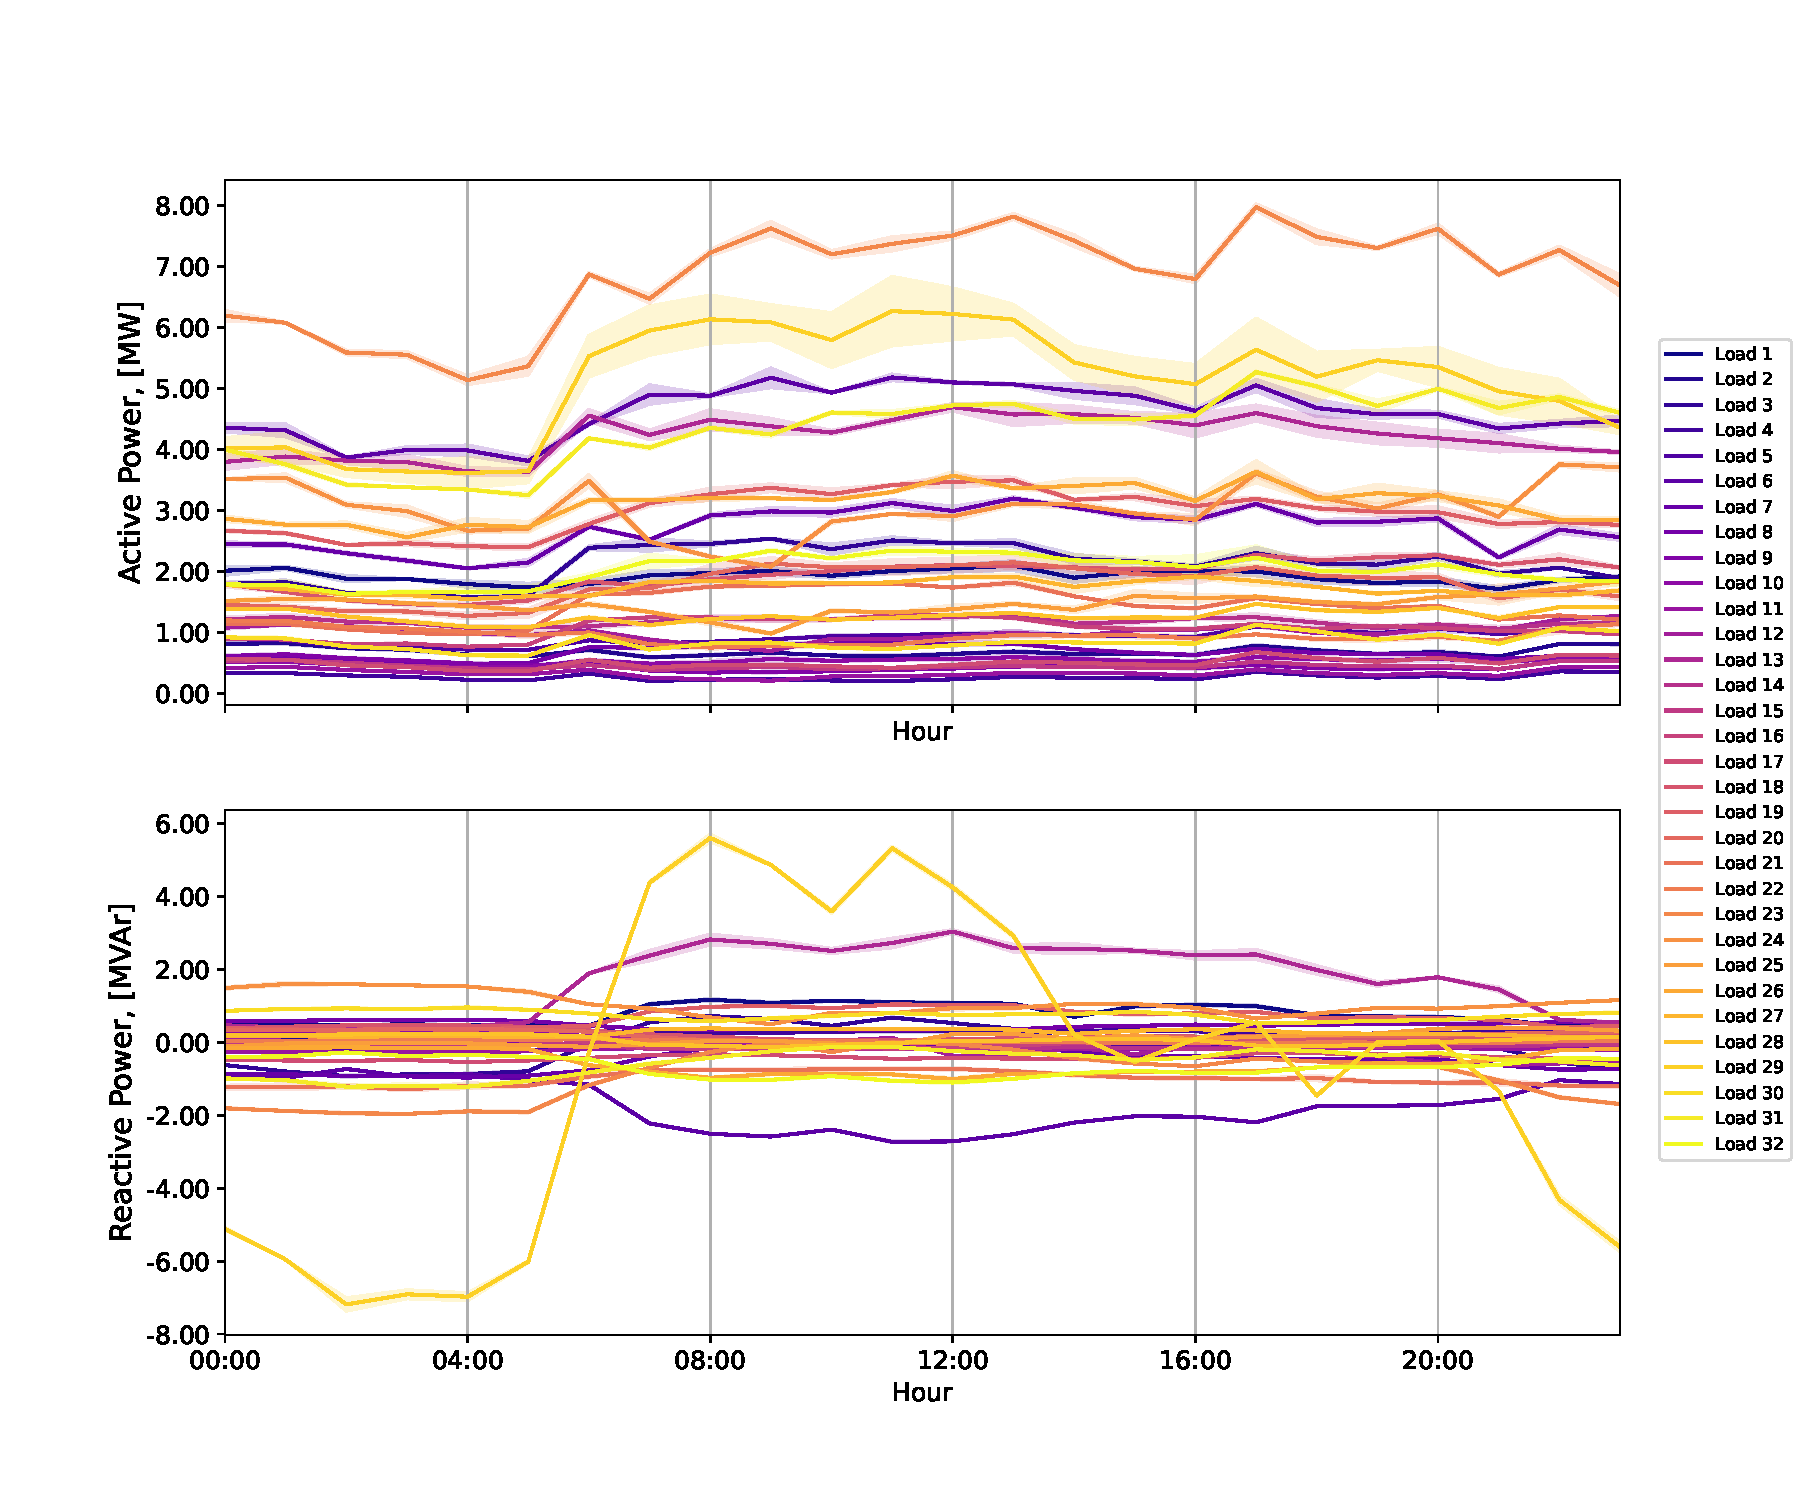
\includegraphics[width=0.475\textwidth]{case33_2_load_scenarios_2025_Autumn.pdf}
    }
    \hfill
    \subfloat[Winter 2025]{
        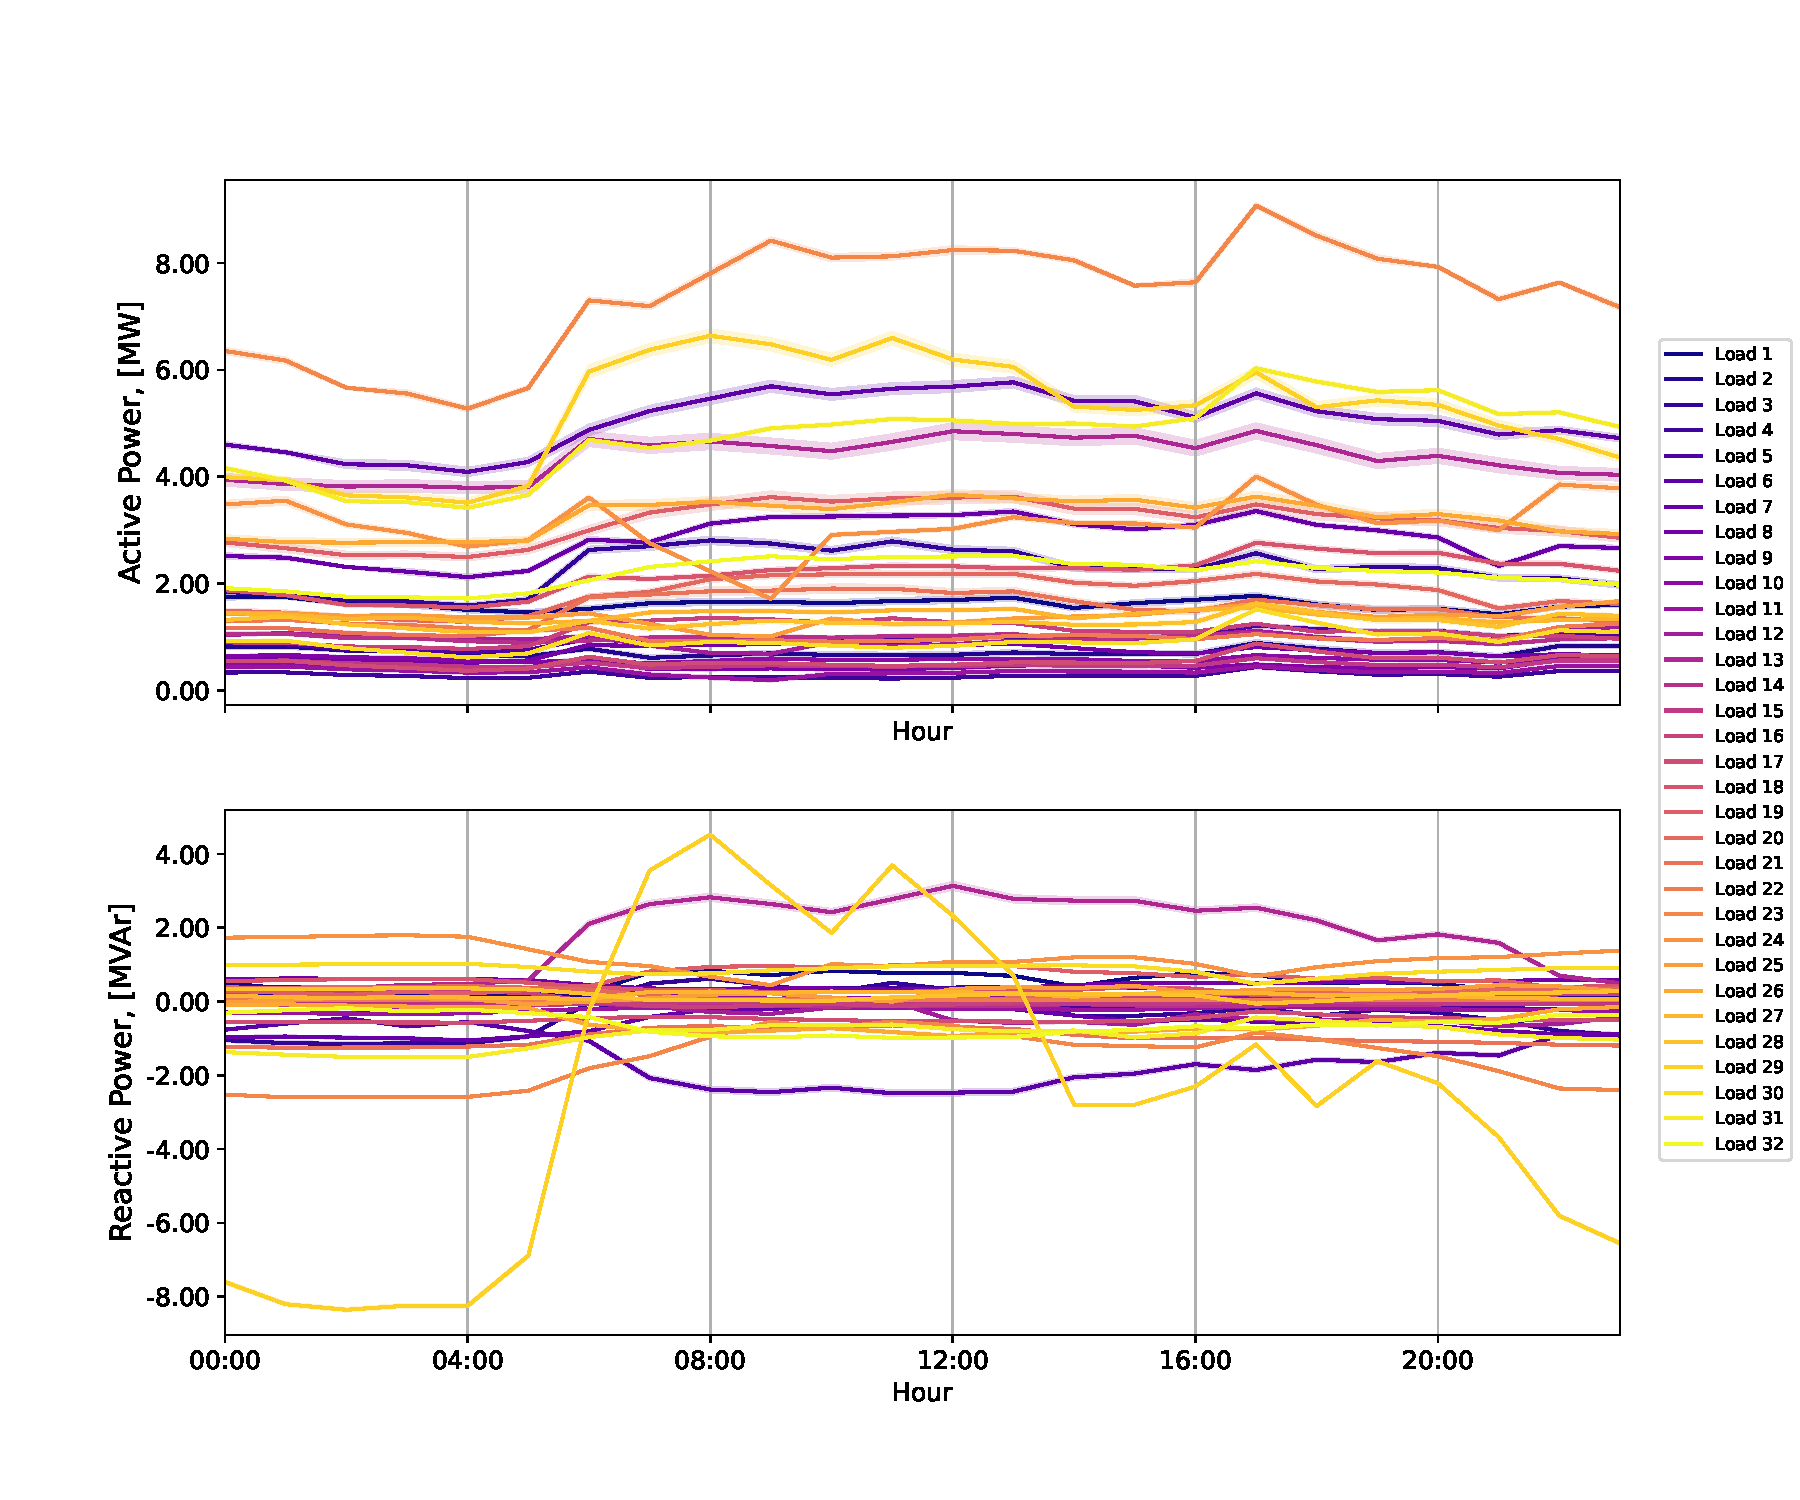
\includegraphics[width=0.475\textwidth]{case33_2_load_scenarios_2025_Winter.pdf}
    }
    \caption{ADN at TN node 7: load profiles for 2025.}
    \label{fig:cs3_adn_node_7_load_scenarios_2025}
\end{figure*}

\begin{figure}[htbp!]
    \centering
    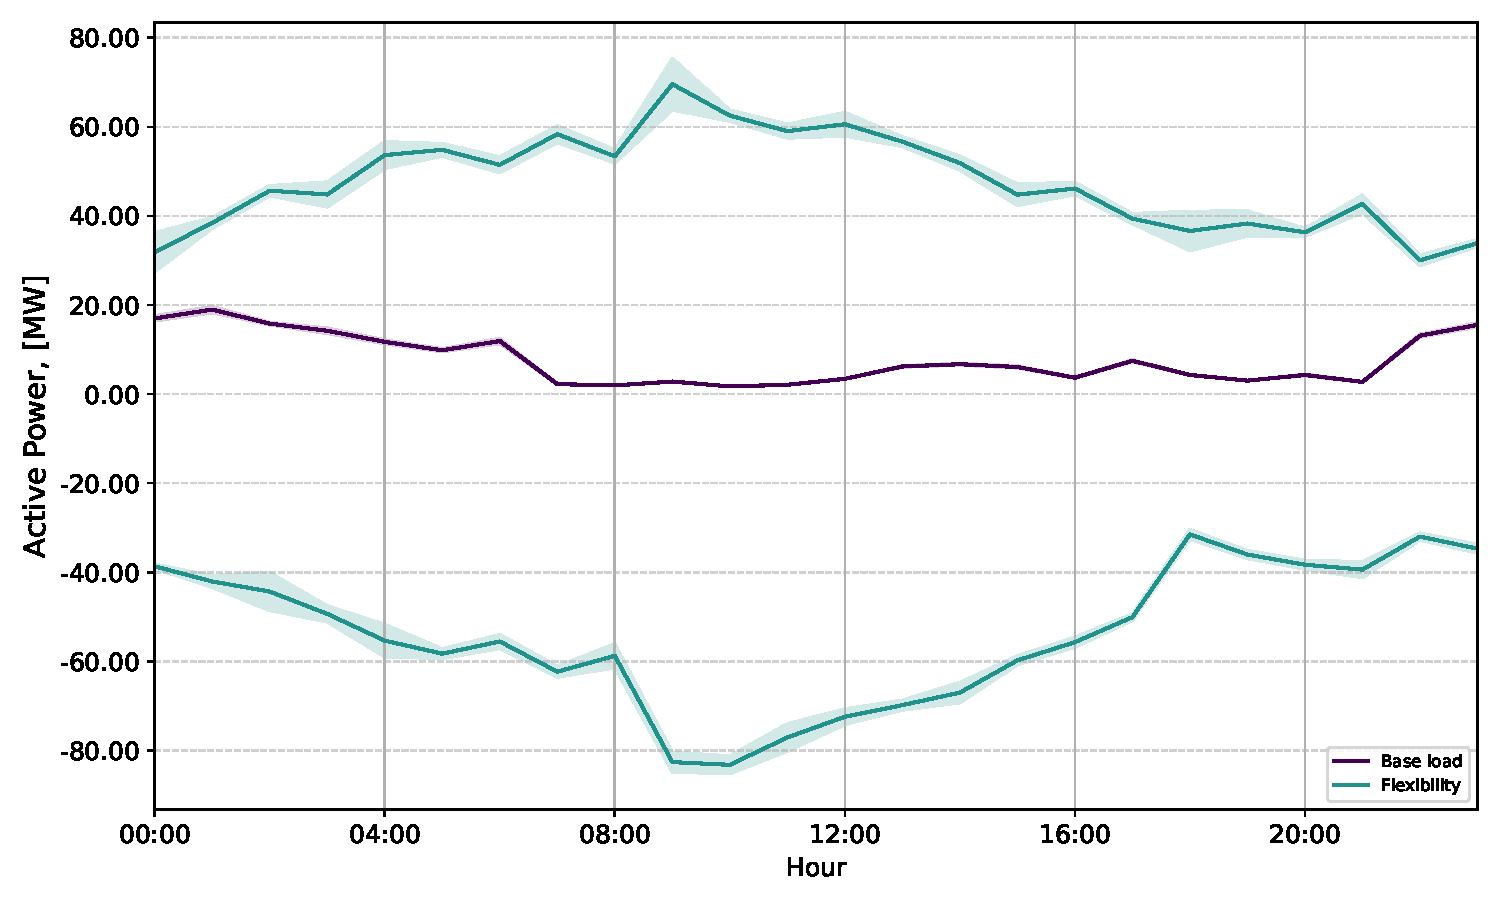
\includegraphics[width=0.65\textwidth]{case33_2_flexibility_scenarios_2025_Spring.pdf}
    \caption{Flexible load profiles for the ADN at TN node~7.}
    \label{fig:cs3_adn_node_7_flexibility}
\end{figure}

\subsection{ADN Connected to TN node~9}
\label{app:adn_node9_description}

Figure~\ref{fig:cs3_adn_node_9_res_scenarios_2025} and Figure~\ref{fig:cs3_adn_node_9_load_scenarios_2025} show the RES generation and load profiles for the spring, summer, autumn, and winter representative days of 2025 for the ADN at TN node~9. Figure~\ref{fig:cs3_adn_node_9_flexibility} shows the flexible load profiles adopted for this ADN.

\begin{figure*}[htbp]
    \centering
    \subfloat[Spring 2025]{
        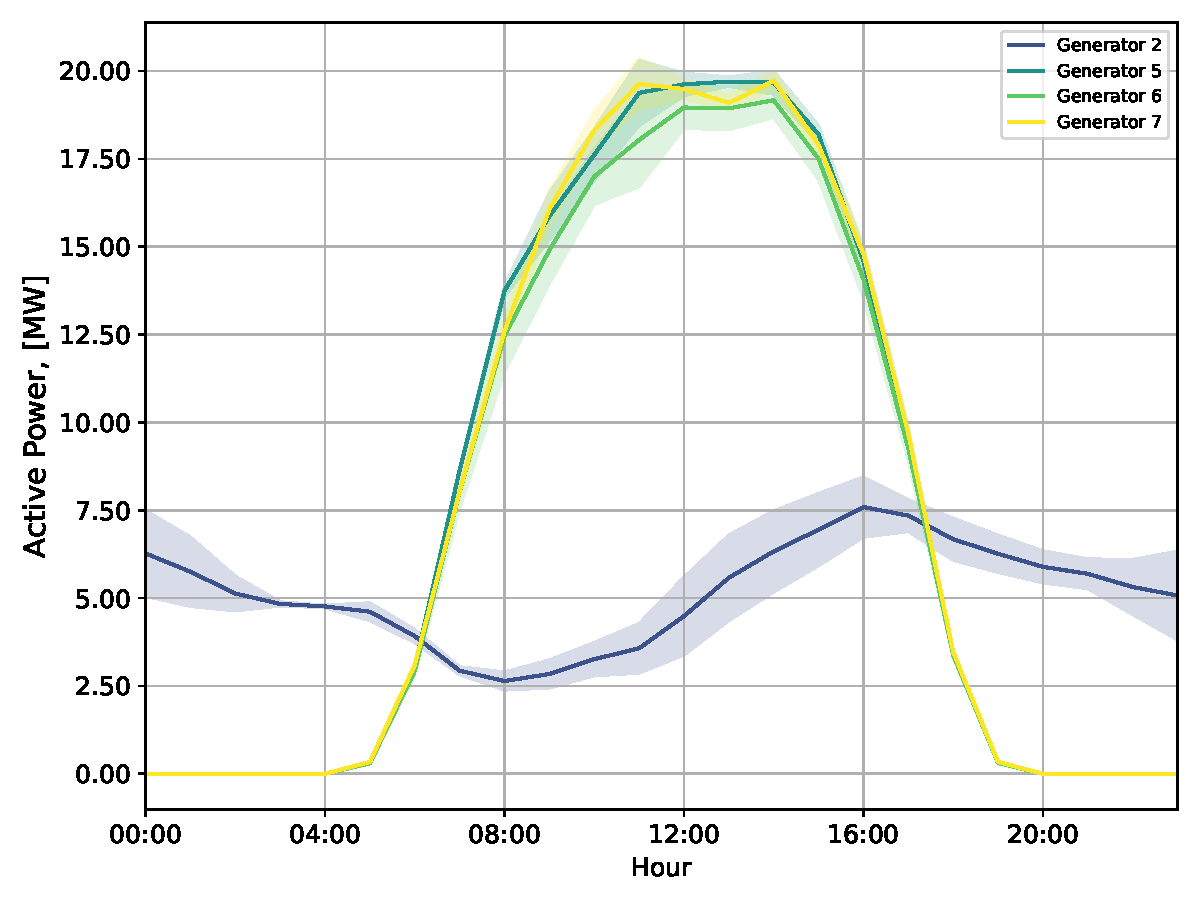
\includegraphics[width=0.475\textwidth]{case33_3_RES_generation_scenarios_2025_Spring.pdf}
    }
    \hfill
    \subfloat[Summer 2025]{
        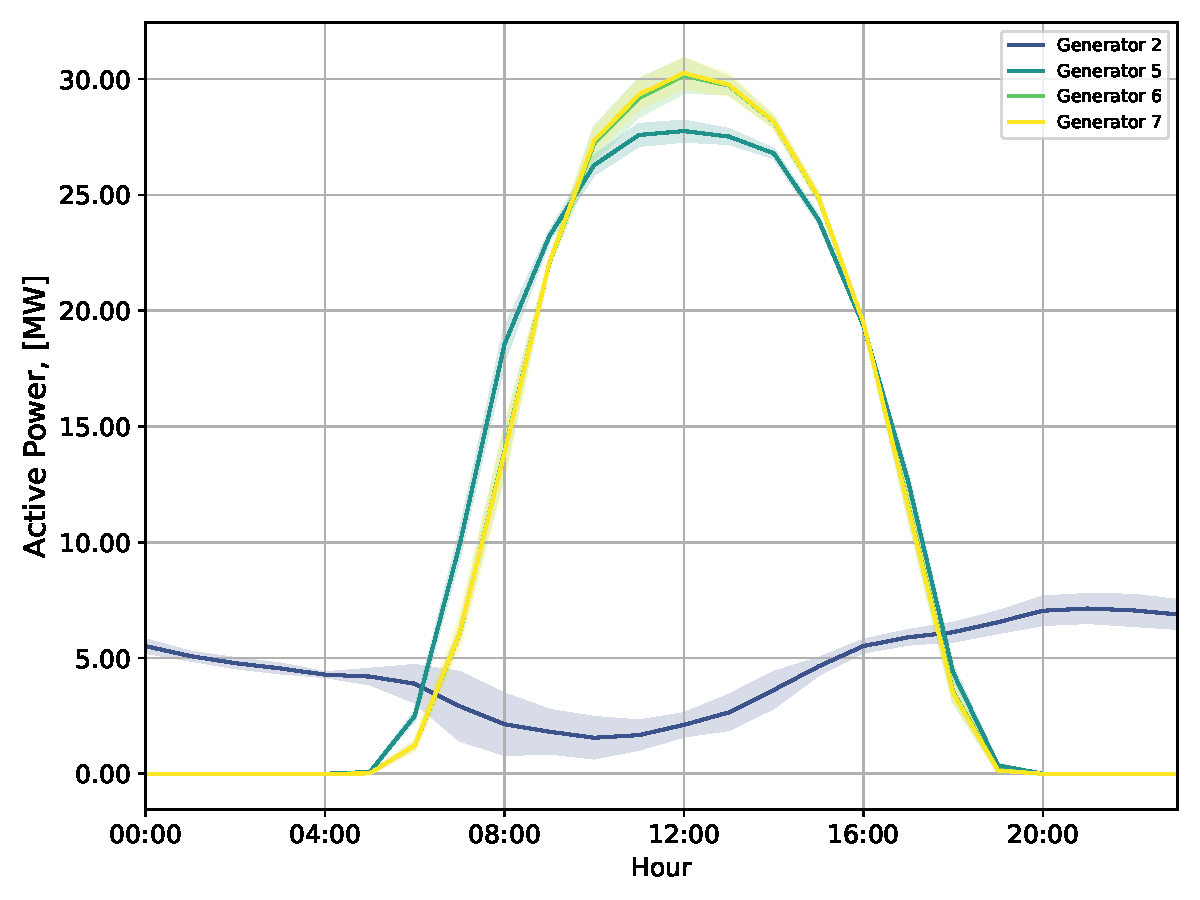
\includegraphics[width=0.475\textwidth]{case33_3_RES_generation_scenarios_2025_Summer.pdf}
    }
    \\[5pt]
    \subfloat[Autumn 2025]{
        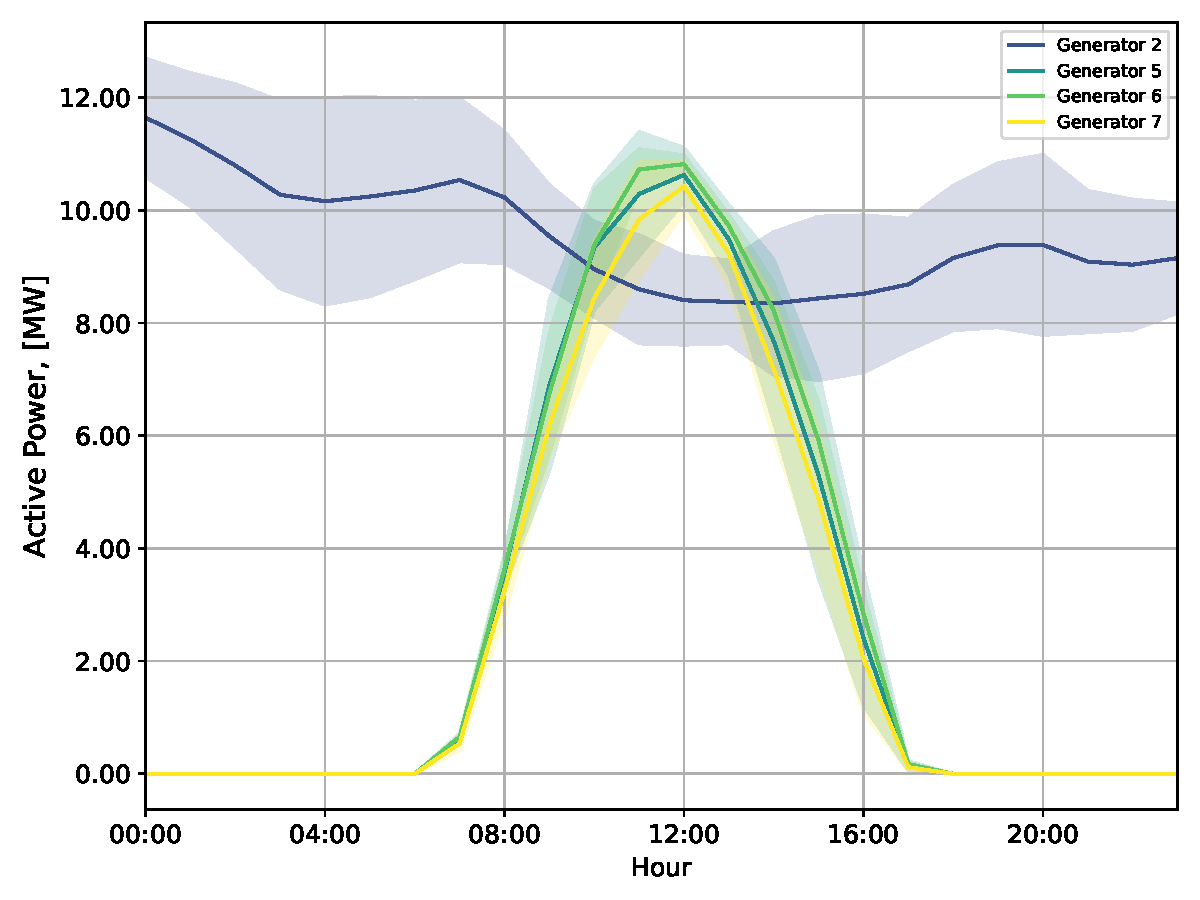
\includegraphics[width=0.475\textwidth]{case33_3_RES_generation_scenarios_2025_Autumn.pdf}
    }
    \hfill
    \subfloat[Winter 2025]{
        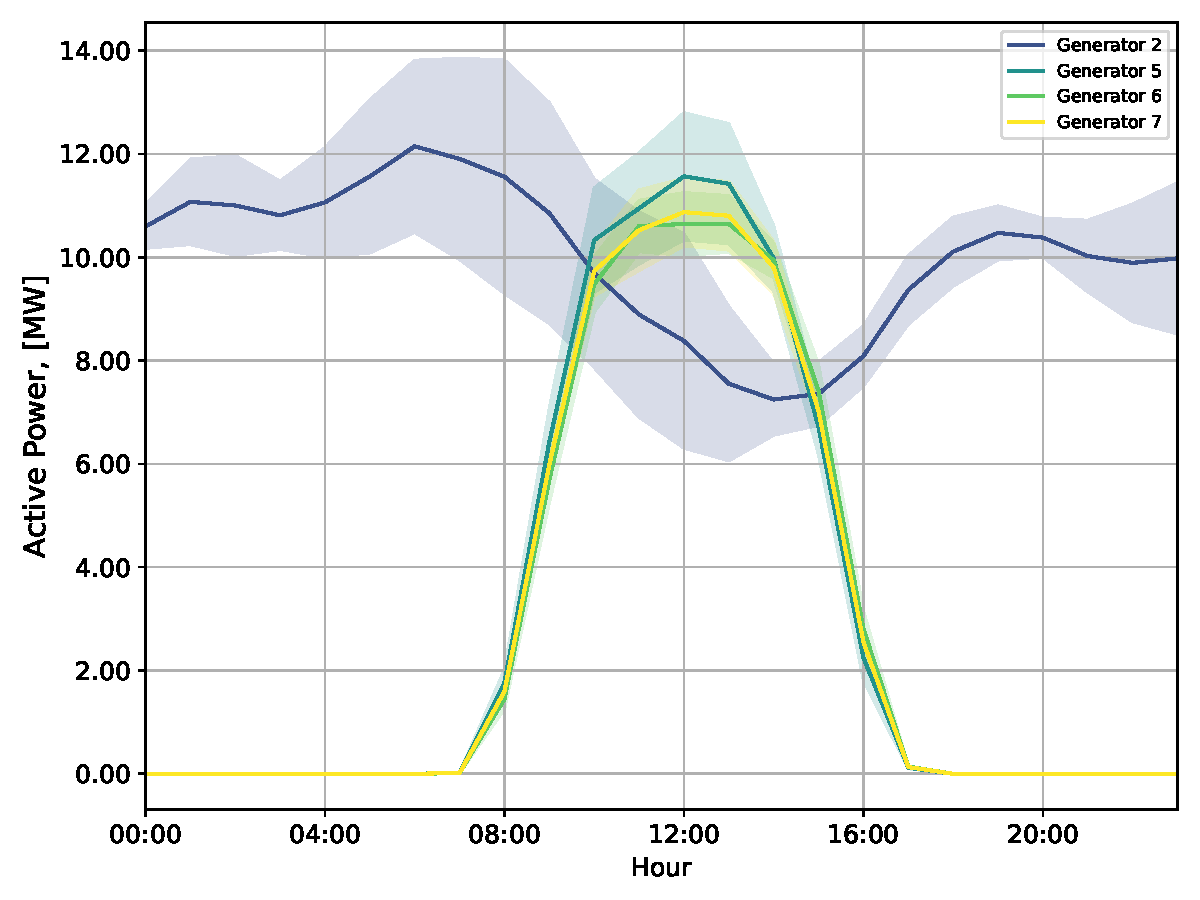
\includegraphics[width=0.475\textwidth]{case33_3_RES_generation_scenarios_2025_Winter.pdf}
    }
    \caption{ADN at TN node 9: RES profiles for 2025.}
    \label{fig:cs3_adn_node_9_res_scenarios_2025}
\end{figure*}

\begin{figure*}[htbp]
    \centering
    \subfloat[Spring 2025]{
        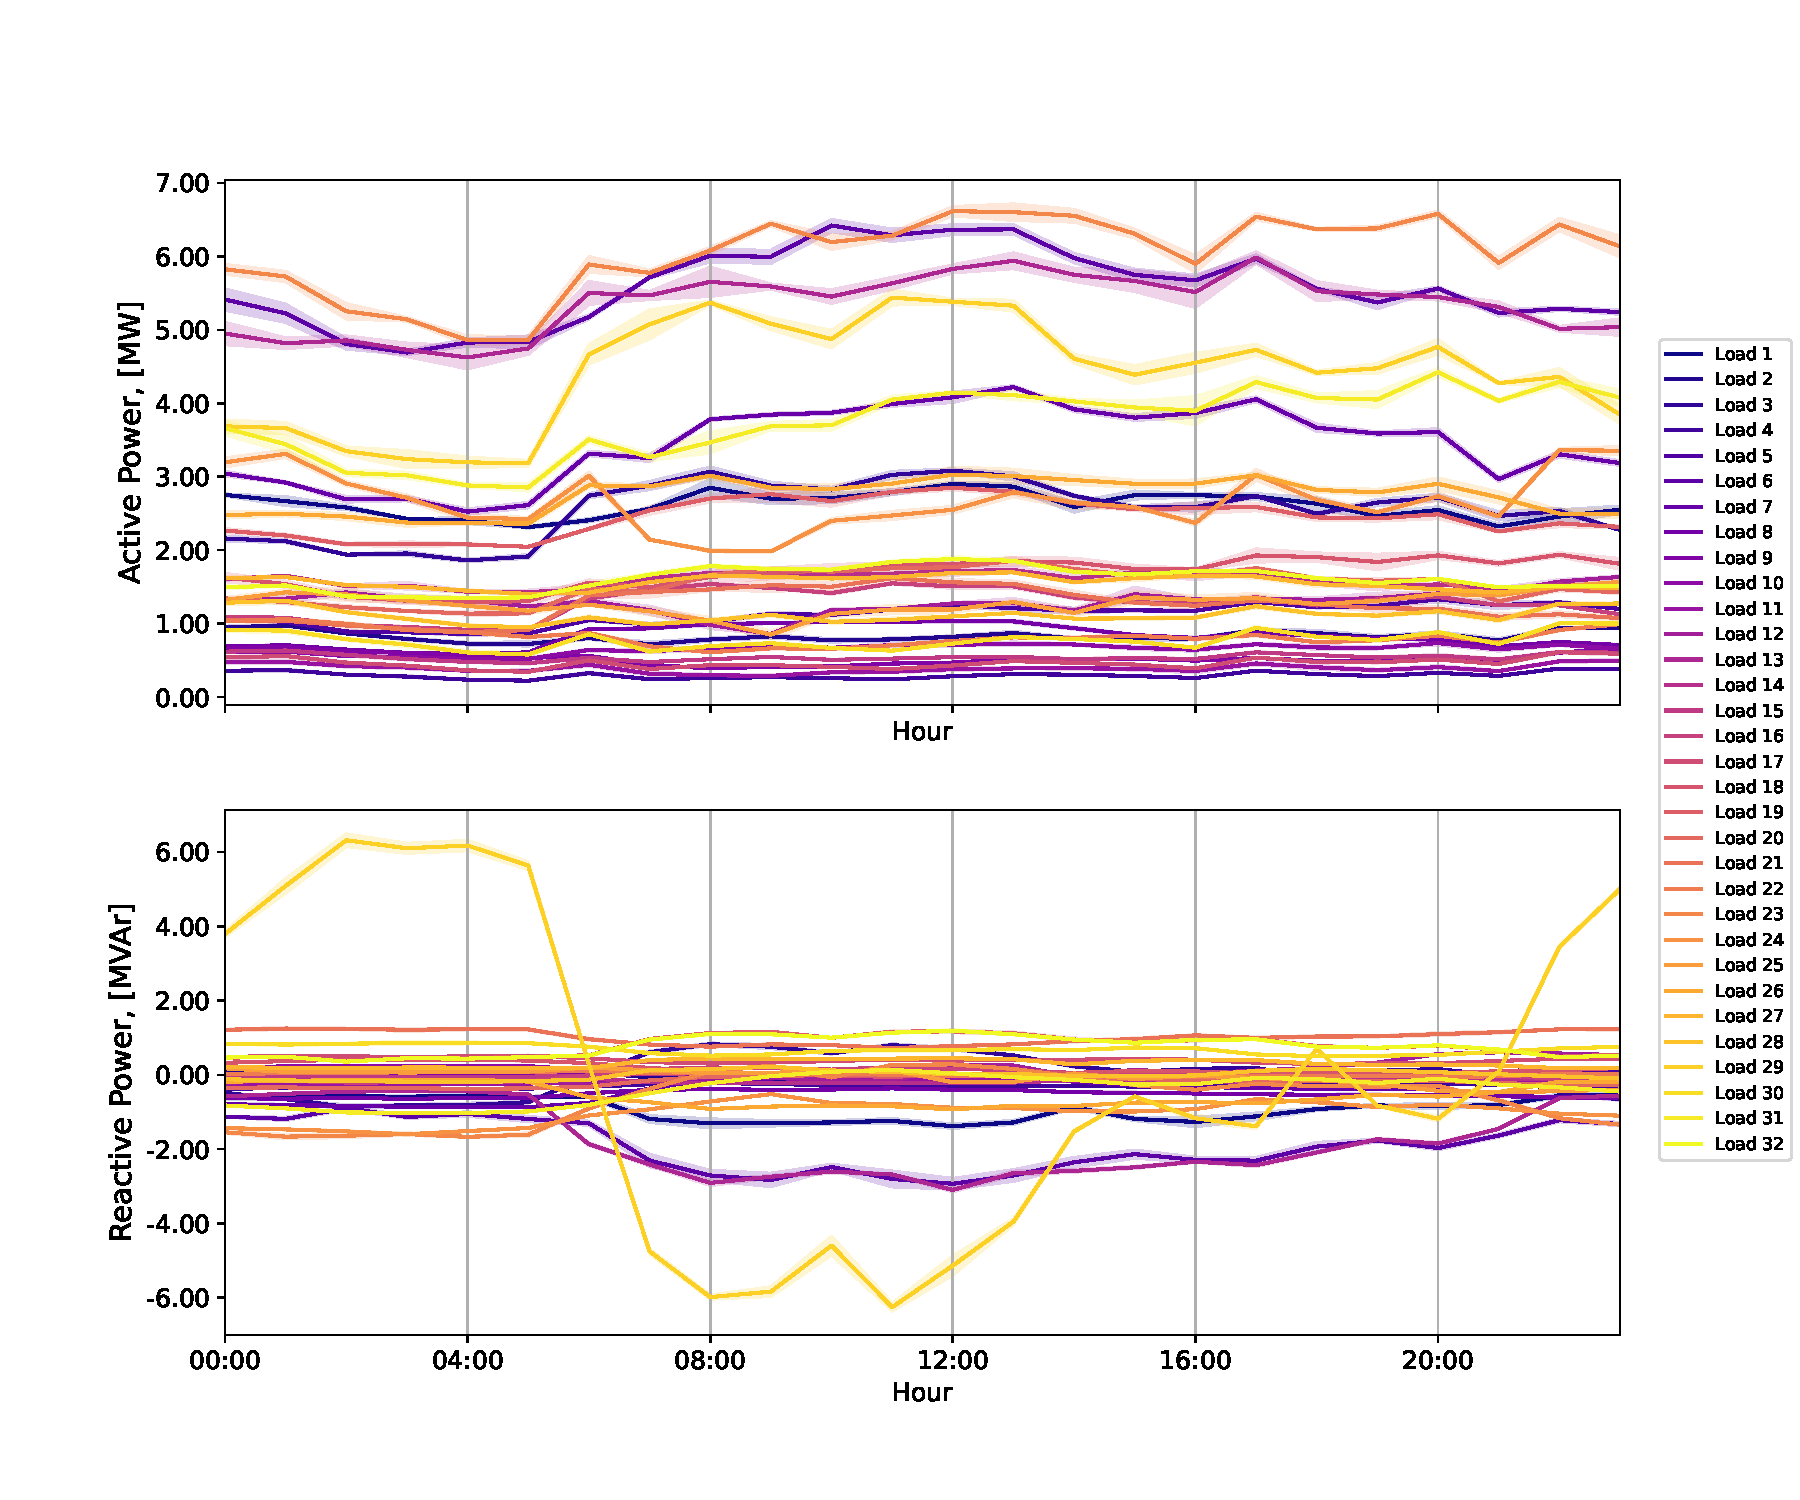
\includegraphics[width=0.475\textwidth]{case33_3_load_scenarios_2025_Spring.pdf}
    }
    \hfill
    \subfloat[Summer 2025]{
        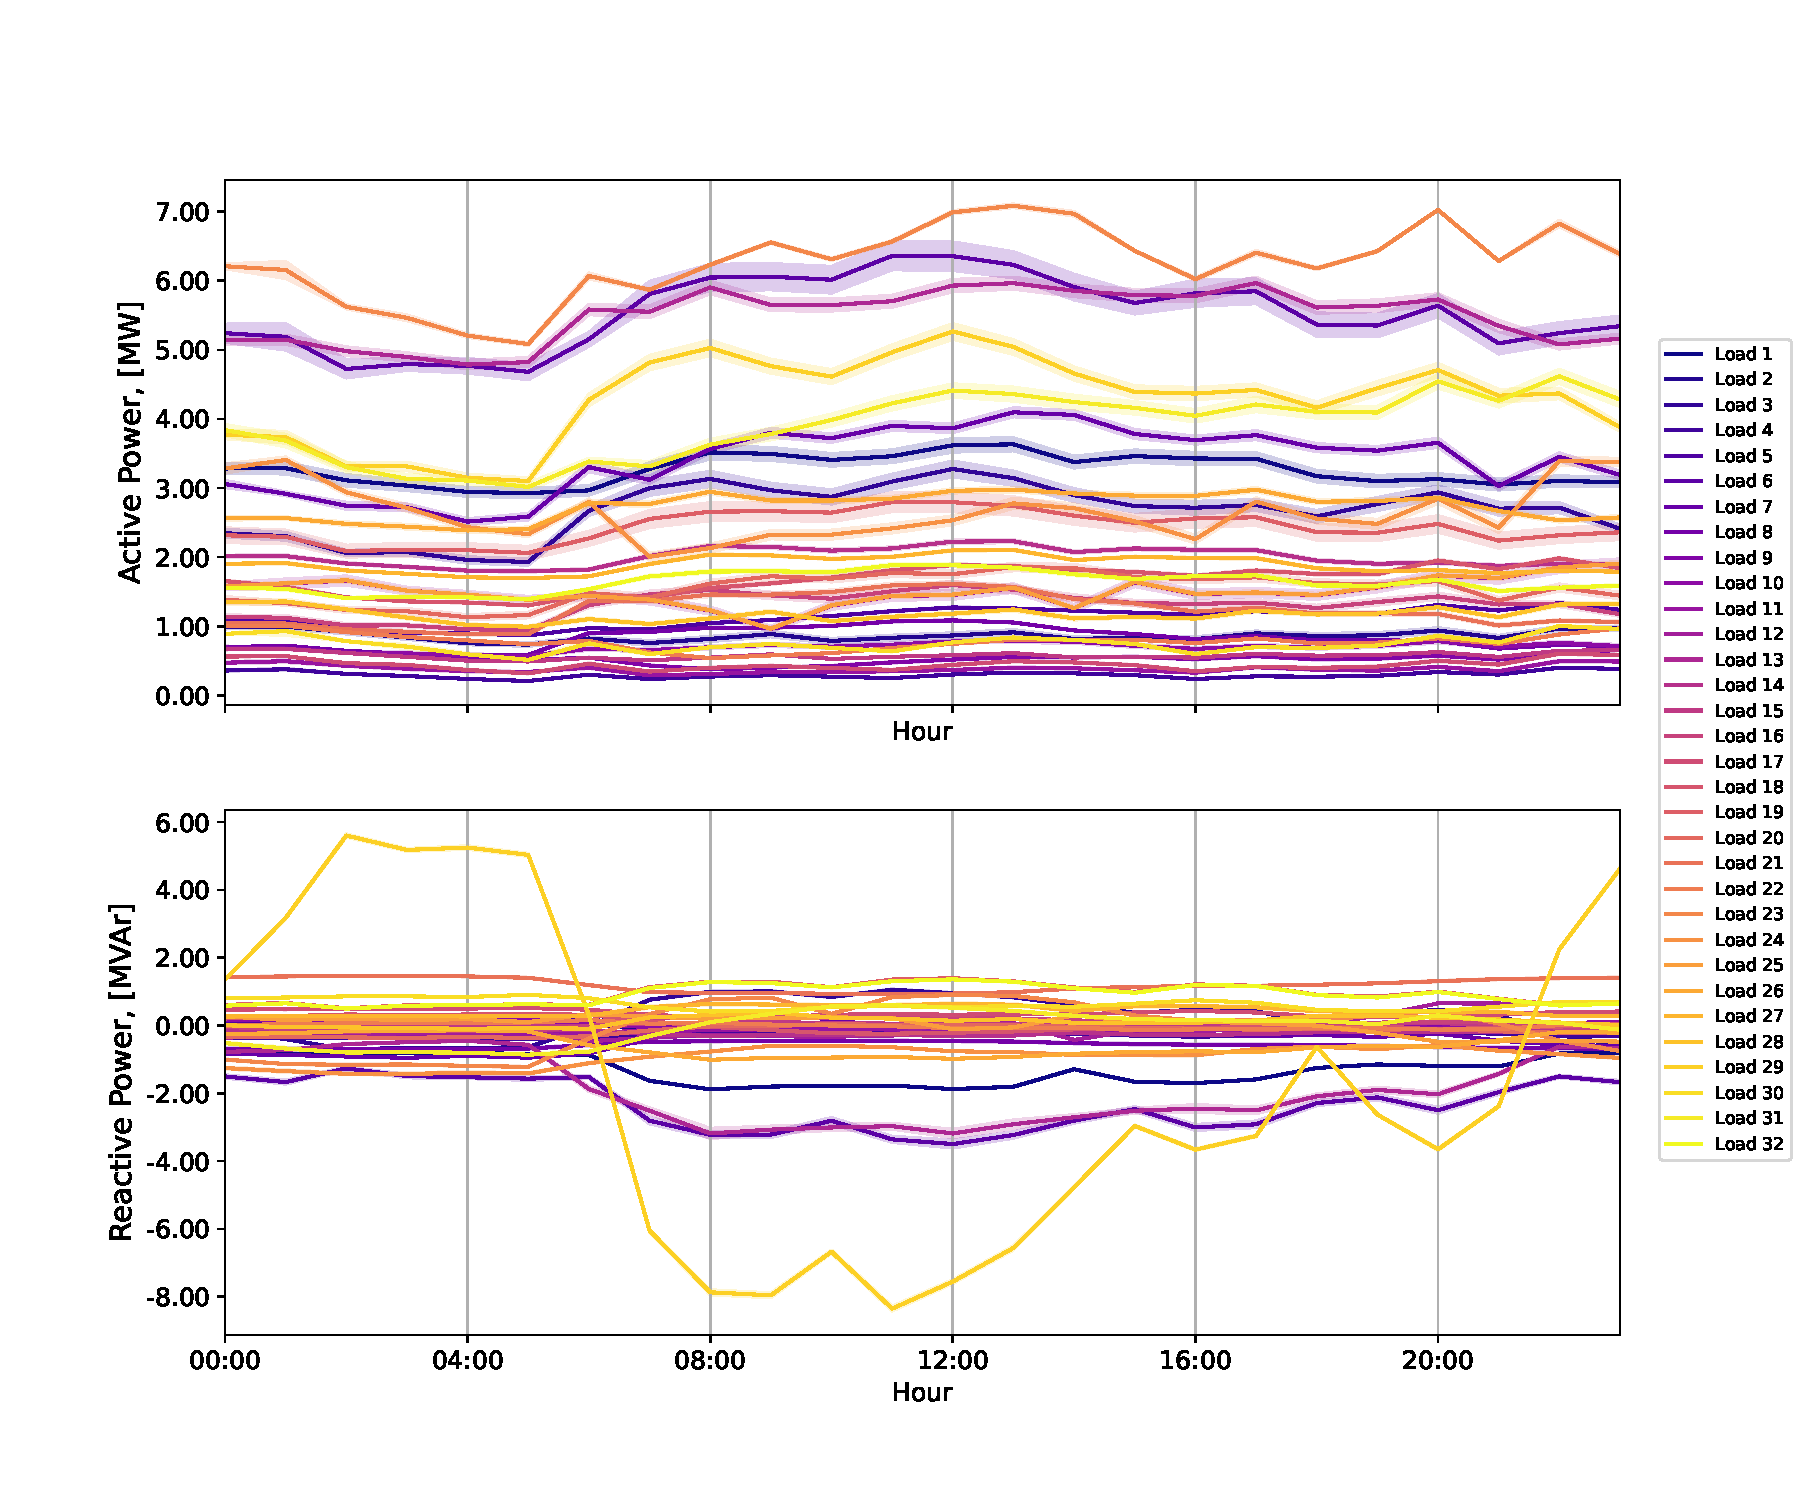
\includegraphics[width=0.475\textwidth]{case33_3_load_scenarios_2025_Summer.pdf}
    }
    \\[5pt]
    \subfloat[Autumn 2025]{
        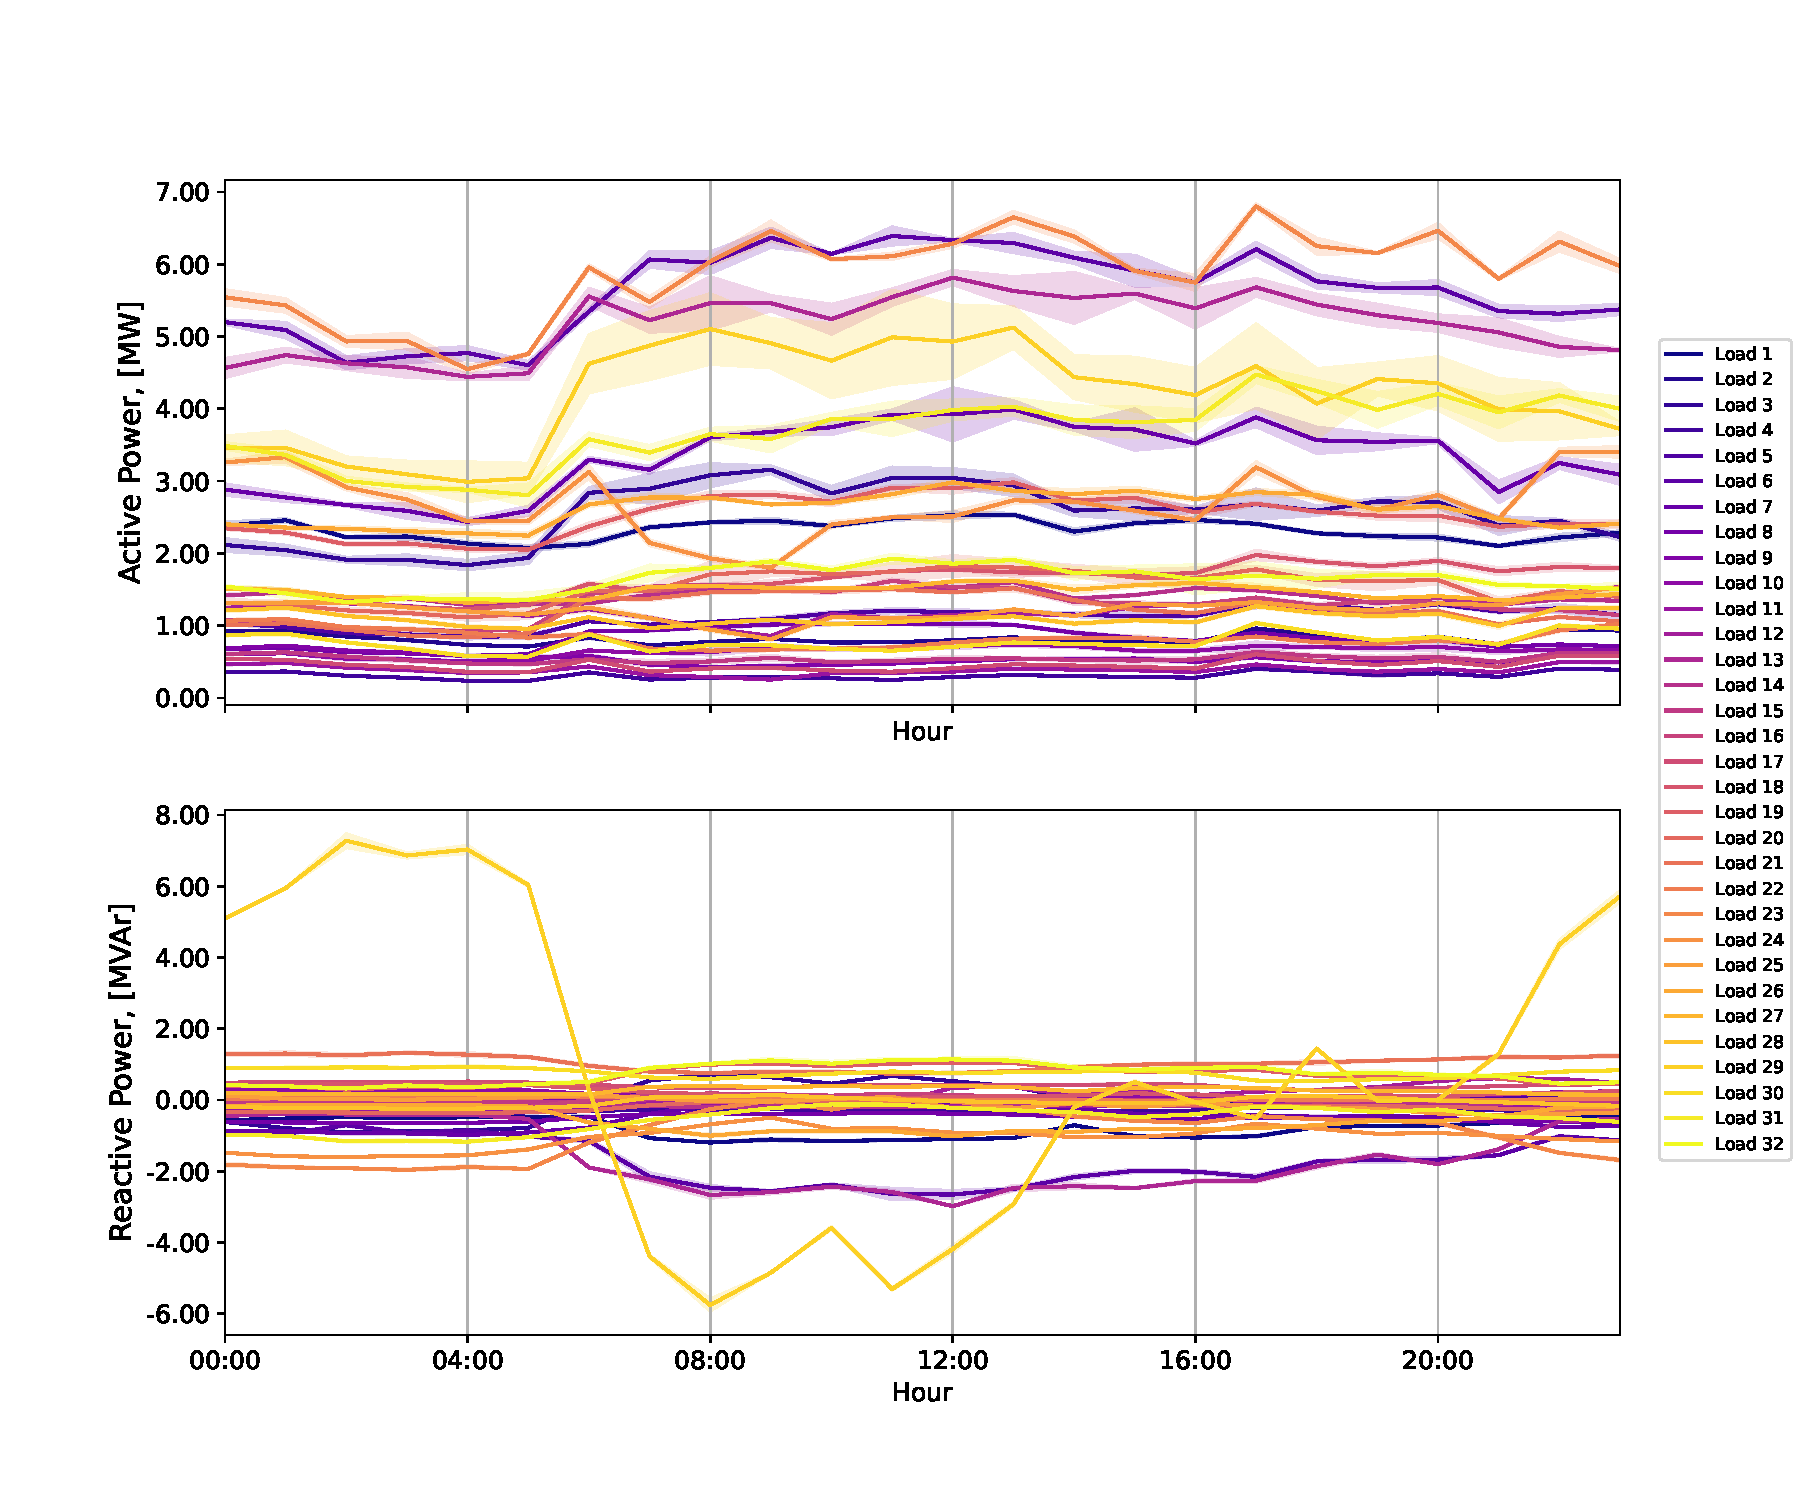
\includegraphics[width=0.475\textwidth]{case33_3_load_scenarios_2025_Autumn.pdf}
    }
    \hfill
    \subfloat[Winter 2025]{
        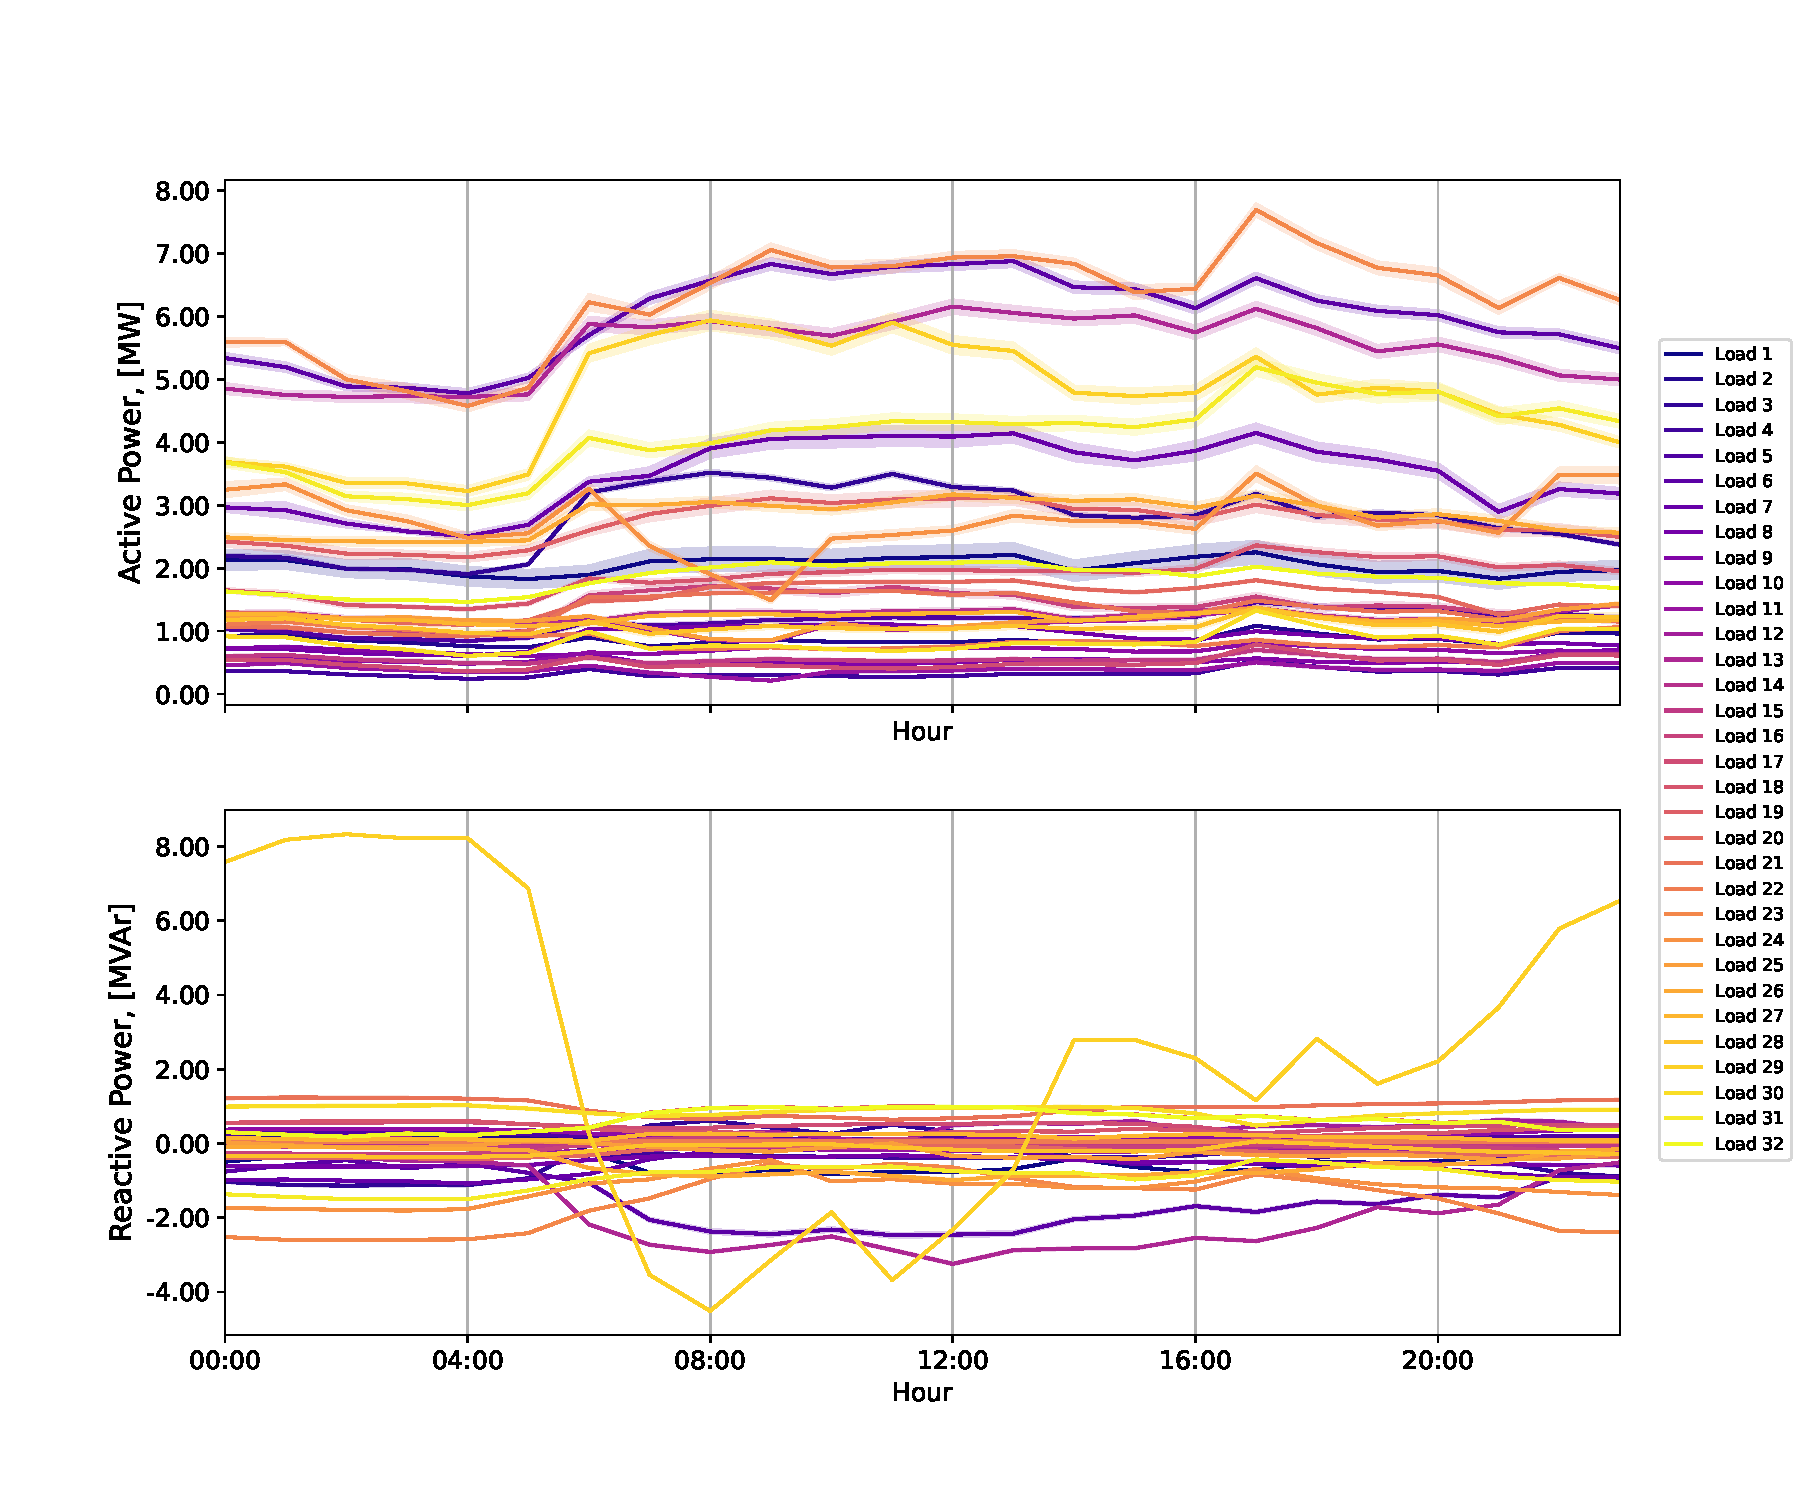
\includegraphics[width=0.475\textwidth]{case33_3_load_scenarios_2025_Winter.pdf}
    }
    \caption{ADN at TN node 9: load profiles for 2025.}
    \label{fig:cs3_adn_node_9_load_scenarios_2025}
\end{figure*}

\begin{figure}[htbp!]
    \centering
    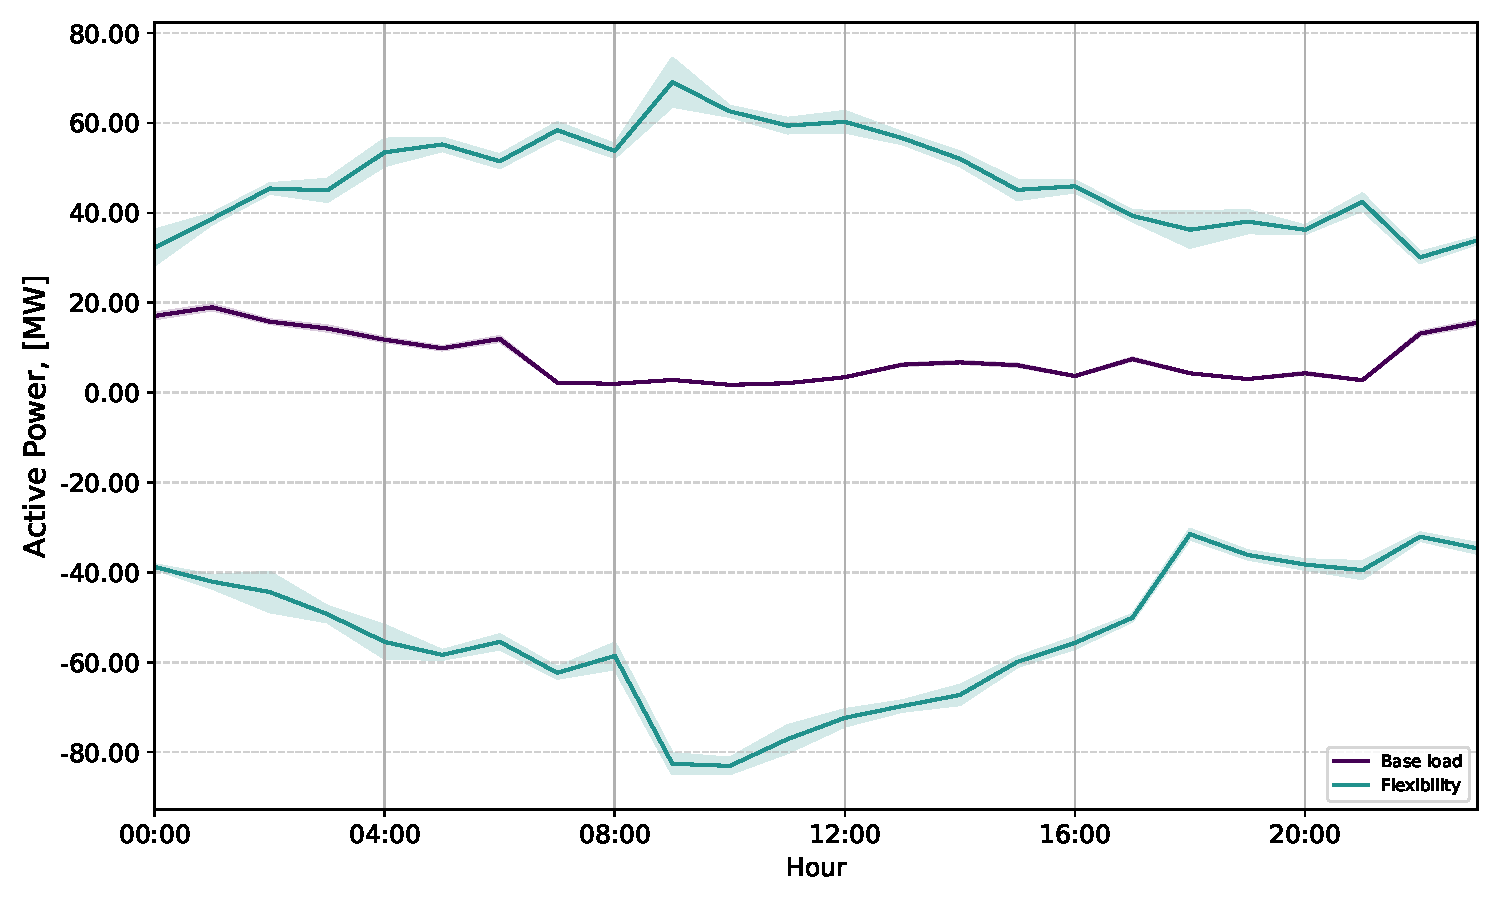
\includegraphics[width=0.65\textwidth]{case33_3_flexibility_scenarios_2025_Spring.pdf}
    \caption{Flexible load profiles for the ADN at TN node~9.}
    \label{fig:cs3_adn_node_9_flexibility}
\end{figure}

\section{Results}
\label{app:results}

Table~\ref{tab:cs3_results_summary_years_days} provides a detailed breakdown of operational costs, RES generation, and RES curtailment for each representative year and season. It complements the aggregated results reported in Section~\ref{sec:results} and enables a more granular assessment of seasonal and inter-annual performance differences across test cases.

\begin{landscape}
    \begin{table}[htbp!]
    \centering
    \caption{Operational planning results by representative year and representative day.}
    \resizebox{1.40\textwidth}{!}{
        \begin{tabular}{lll cccc c cccc c cccc c cccc c cccc}
            \toprule
            ~ & ~ & ~ & \multicolumn{4}{c}{2025} & ~ & \multicolumn{4}{c}{2028} & ~ & \multicolumn{4}{c}{2031} & ~ & \multicolumn{4}{c}{2034} & ~ & \multicolumn{4}{c}{2037}\\
            \cmidrule{4-7} \cmidrule{9-12} \cmidrule{14-17} \cmidrule{19-22} \cmidrule{24-27}
            ~ & ~ & ~ & Spring & Summer & Autumn & Winter &  
                      & Spring & Summer & Autumn & Winter &  
                      & Spring & Summer & Autumn & Winter & 
                      & Spring & Summer & Autumn & Winter & 
                      & Spring & Summer & Autumn & Winter \\
            \midrule
            \multicolumn{3}{l}{Uncoordinated}\\ \cmidrule{2-27}
            ~ & \multicolumn{2}{l}{Operational Cost, [\euro]}   & 269671.54 & 240359.85 & 194686.35 & 207466.96 & ~
                                                                & 278745.92 & 271843.10 & 239972.27 & 247310.67 & ~
                                                                & 266821.42 & 241056.10 & 178945.77 & 159305.51 & ~
                                                                & 313102.26 & 288405.93 & 179448.50 & 209415.34 & ~
                                                                & 329528.87 & 294022.70 & 195895.18 & 275763.44\\
            ~ & \multicolumn{2}{l}{RES Generation, [MWh]}       & 814.83 & 875.19 & 907.46 & 1074.27 & ~
                                                                & 799.59 & 871.78 & 1038.93 & 1140.19 & ~
                                                                & 1170.76 & 1106.34 & 1547.14 & 1573.34 & ~
                                                                & 1227.64 & 1206.71 & 1462.45 & 1631.29 & ~
                                                                & 1177.36 & 927.30 & 1831.44 & 1322.29\\
            ~ & \multicolumn{2}{l}{RES Curtailment, [MVAh]}     & 0.00 & 5.22 & 0.00 & 0.00 & ~
                                                                & 10.98 & 0.00 & 0.00 & 0.00 & ~
                                                                & 84.56 & 240.34 & 0.00 & 0.00 & ~
                                                                & 57.84 & 159.49 & 0.00 & 0.00 & ~
                                                                & 316.18 & 697.68 & 0.00 & 624.33\\
            \midrule
            \multicolumn{3}{l}{Without Shared ESSs}\\ \cmidrule{2-27}
            ~ & \multicolumn{2}{l}{Operational Cost}\\       
            ~ & ~ & Total, [\euro]  & 244253.20 & 235518.58 & 200807.07 & 208417.00 & ~
                                    & 248518.89 & 259801.27 & 245425.14 & 249162.75 & ~ 
                                    & 231386.32 & 229083.91 & 184500.25 & 162710.69 & ~ 
                                    & 274169.86 & 272988.69 & 187791.61 & 211915.70 & ~
                                    & 270509.42 & 247965.68 & 205275.47 & 189951.70\\
            ~ & ~ & Variation, [\%] & -9.43\% & -2.01\% & 3.14\% & 0.46\% & ~ 
                                    & -10.84\% & -4.43\% & 2.27\% & 0.75\% & ~
                                    & -13.28\% & -4.97\% & 3.10\% & 2.14\% & ~ 
                                    & -12.43\% & -5.35\% & 4.65\% & 1.19\% & ~
                                    & -17.91\% & -15.66\% & 4.79\% & -31.12\%\\ \cmidrule{2-27}
            ~ & \multicolumn{2}{l}{RES Generation}\\
            ~ & ~ & Total, [MWh] & 795.04 & 867.14 & 894.16 & 1076.33 & ~
                                 & 773.76 & 856.18 & 1025.98 & 1137.93 & ~ 
                                 & 1218.67 & 1335.05 & 1538.91 & 1569.59 & ~ 
                                 & 1259.00 & 1353.06 & 1451.31 & 1626.96 & ~
                                 & 1405.13 & 1537.88 & 1825.09 & 1944.63\\
            ~ & ~ & Variation, [\%] & -2.43\% & -0.92\% & -1.47\% & 0.19\% & ~ 
                                    & -3.23\% & -1.79\% & -1.25\% & -0.20\% & ~ 
                                    & 4.09\% & 20.67\% & -0.53\% & -0.24\% & ~ 
                                    & 2.56\% & 12.13\% & -0.76\% & -0.27\% & ~ 
                                    & 19.35\% & 65.85\% & -0.35\% & 47.07\%\\
            \cmidrule{2-27}
            ~ & \multicolumn{2}{l}{RES Curtailment}\\       
            ~ & ~ & Total, [MVAh]  & 19.76 & 13.29 & 13.25 & 5.41 & ~ 
                                  & 36.80 & 15.56 & 12.90 & 5.79 & ~ 
                                  & 36.66 & 12.18 & 8.19 & 3.70 & ~
                                  & 26.48 & 13.21 & 11.10 & 4.29 & ~
                                  & 88.47 & 87.80 & 7.13 & 3.72\\
            ~ & ~ & Variation, [\%] & N/A & 154.45\% & N/A & N/A & ~ 
                                    & 235.22\% & N/A & N/A & N/A & ~ 
                                    & -56.65\% & -94.93\% & N/A & N/A & ~
                                    & -54.22\% & -91.72\% & N/A & N/A & ~
                                    & -72.02\% & -87.42\% & N/A & -99.40\%\\
            \midrule
            \multicolumn{3}{l}{With Shared ESSs}\\ \cmidrule{2-27}
            ~ & \multicolumn{2}{l}{Operational Cost}\\   
            ~ & ~ & Total, [\euro]  & 244140.90 & 234804.95 & 200439.69 & 209948.35 & ~
                                    & 246055.36 & 258220.48 & 245809.26 & 249029.65 & ~ 
                                    & 233458.63 & 227967.81 & 186566.71 & 160903.39 & ~ 
                                    & 284765.82 & 272862.03 & 187353.93 & 212285.38 & ~ 
                                    & 269546.16 & 233501.93 & 203314.34 & 188930.78\\
            ~ & ~ & Variation, [\%] & -9.47\% & -2.31\% & 2.96\% & 1.20\% & ~ 
                                    & -11.73\% & -5.01\% & 2.43\% & 0.70\% & ~
                                    & -12.50\% & -5.43\% & 4.26\% & 1.00\% & ~ 
                                    & -9.05\% & -5.39\% & 4.41\% & 1.37\% & ~ 
                                    & -18.20\% & -20.58\% & 3.79\% & -31.49\%\\ \cmidrule{2-27}
            ~ & \multicolumn{2}{l}{RES Generation}\\       
            ~ & ~ & Total, [MWh] & 795.03 & 867.15 & 894.17 & 1076.34 & ~ 
                                 & 773.74 & 856.20 & 1025.95 & 1137.90 & ~ 
                                 & 1218.68 & 1334.90 & 1538.84 & 1569.55 & ~ 
                                 & 1212.29 & 1353.10 & 1451.27 & 1626.96 & ~ 
                                 & 1405.29 & 1597.11 & 1825.09 & 1944.64\\
            ~ & ~ & Variation, [\%] & -2.43\% & -0.92\% & -1.47\% & 0.19\% & ~
                                    & -3.23\% & -1.79\% & -1.25\% & -0.20\% & ~
                                    & 4.09\% & 20.66\% & -0.54\% & -0.24\% & ~
                                    & -1.25\% & 12.13\% & -0.76\% & -0.27\% & ~
                                    & 19.36\% & 72.23\% & -0.35\% & 47.07\%\\ \cmidrule{2-27}
            ~ & \multicolumn{2}{l}{RES Curtailment}\\       
            ~ & ~ & Total, [MVAh] & 19.77 & 13.28 & 13.25 & 5.41 & ~
                                  & 36.82 & 15.55 & 12.87 & 5.78 & ~
                                  & 36.63 & 12.30 & 8.21 & 3.75 & ~
                                  & 73.17 & 13.16 & 11.14 & 4.29 & ~
                                  & 88.31 & 28.58 & 7.12 & 3.70\\
            ~ & ~ & Variation, [\%] & N/A & 154.19\% & N/A & N/A & ~
                                    & 235.43\% & N/A & N/A & N/A & ~
                                    & -56.68\% & -94.88\% & N/A & N/A & ~
                                    & 26.49\% & -91.75\% & N/A & N/A & ~
                                    & -72.07\% & -95.90\% & N/A & -99.41\%\\
            \bottomrule
        \end{tabular}
    }
    \label{tab:cs3_results_summary_years_days}
    \end{table}
\end{landscape}

\section*{Declaration of generative AI and AI-assisted technologies in the manuscript preparation process}

During the preparation of this work the author(s) used ChatGPT in order to improve readability and language in selected parts of the manuscript. After using this tool, the author(s) reviewed and edited the content as needed and take full responsibility for the content of the published article.

% ====================================================================================================================
%                                                     BIBLIOGRAPHY                                                    
% ====================================================================================================================
\bibliographystyle{elsarticle-num} 
\bibliography{bibliography}

\end{document}

\endinput
%%
%% End of file `elsarticle-template-num.tex'.
